\documentclass[12pt,a4paper]{article}

\usepackage[OT1]{fontenc}
\usepackage[utf8]{inputenc}
\usepackage[russian,english]{babel}
%%%% Additional part of preamble generated by package Sweave in RStudio
%% initial declaration for fonts
\usepackage[labelfont=bf]{caption}
\usepackage[font=small,labelfont=bf]{subcaption}

% for testing
\usepackage{lipsum}

%% For tables
\usepackage{array}
\usepackage{longtable}
\usepackage{fullpage}
\usepackage{dcolumn}
\usepackage[flushleft]{threeparttable}
\usepackage{booktabs}
\usepackage[12hr]{datetime}
\usepackage[DIV=16]{typearea}
\usepackage{scrextend,booktabs}
\usepackage{tabulary}
\usepackage{multirow}
\usepackage[font=footnotesize]{caption}
\usepackage{lscape}

%% Additional elements for figures and numbering added by Sweave
\usepackage{float}
\usepackage[sc]{mathpazo}
\usepackage{geometry}
\geometry{verbose,tmargin=2.5cm,bmargin=2.5cm,lmargin=2.5cm,rmargin=2.5cm}
\setcounter{secnumdepth}{2}
\setcounter{tocdepth}{2}
\usepackage{url}

%% Additional links for hyperref
\usepackage[unicode=true,pdfusetitle,
 bookmarks=true,bookmarksnumbered=true,bookmarksopen=true,bookmarksopenlevel=2,
 breaklinks=false,pdfborder={0 0 1},backref=false,colorlinks=false]
 {hyperref}
\hypersetup{
 pdfstartview={XYZ null null 1}}

\usepackage{breakurl}
\usepackage{Sweave}

%% For math equations
\usepackage{amsmath}
\numberwithin{equation}{section}

%% For bookmarks
\usepackage{bookmark} 

\usepackage[backend=bibtex,
			natbib=true, 
			style=chicago-authordate]{biblatex}
\addbibresource{Returns.bib}


%% For figures numbered by section
\usepackage{chngcntr}
\counterwithin{figure}{section}
\counterwithin{table}{section}

%% For color in text
\usepackage{xcolor}

\begin{document}

\title{Working Paper 1: Returns to Education in the Russian Federation - First Draft \footnote{Arranged in alphabetical order of author last names. The entire code used to generate the graphs and tables presented in this paper is available on bitbucket at \burl{https://bitbucket.org/zagamog/edreru/src/master/} , starting from the raw RLMS data graciously provided in the public domain by the National Research University-Higher School of Economics (HSE).}}
\author{Ekaterina Melianova, Suhas D. Parandekar, Harry A. Patrinos, Art\"{e}m Volgin}
\maketitle

\begin{abstract}
This is the second cut at Working Paper 1 (of proposed 3 working papers) on the Returns of Education in the Russian Federation. The paper shows an interesting pattern of variation in the returns to education from 1994-2018. The paper shows the co-movement of returns to higher education and the return to vocational education. From a policy viewpoint, it shows that returns to education may be strongly influencing decisions of individuals or families regarding their future education trajectories. Policy initiatives seeking to influence enrollment trends at specific educational levels would need to consider the empirical antecedents. 
\end{abstract}


\section{Returns to Education in the Russian Federation: \\ General View}

\subsection{Motivation}

Here there will be 2-3 pages drawn from the CN.
Somewhere we will cite \parencite{mincer_082._1974}. 

\subsection{Data}

For country level analysis, we use the Russian Longitudinal Monitoring Survey (RLMS) - the only representative Russian survey with a sizable panel component allowing for a dynamic analysis \parencite{kozyreva_081._2015}. The data are notable for their reliability, diversity, and applicability to a variety of research questions. The RLMS embraces information on people's income and expenditure structure, their material well-being, educational and occupational behavior, health state and nutrition, migration, etc.  RLMS sampling procedures have been thoroughly and extensively described elsewhere \parencite{kozyreva_081._2015}. The present research uses all 23 waves (1994 - 2018) that are available as of \today. The sub-sample selected for empirical investigation in this paper consists of working individuals aged 25-64 who are out of school and have positive labor market experience and income. 
\\

\subsection{Estimation}

Our empirical analysis present results for the general working population of the Russian Federation aged 25-64 and by gender. We use a basic Mincerian specification shown in equation \eqref{eq:1.1}: 


\begin{flalign}\label{eq:1.1} 
Log(Wage) = b_0 + b_1\cdot Educ + b_2\cdot Exp + b_3\cdot Exp^2 + b_4\cdot Gender + \epsilon
\end{flalign}



\noindent
where $Log(Wage)$ is a logarithm of monthly wage, $Educ$ stands for the years of education or highest attained level of education, $Exp$ and $Exp^2$ reflect the years of working experience and its quadratic term respectively, $Gender$ is a dummy variable for gender, $b_0$ is an intercept, $b_1 ... b_n$ are the respective slope estimates, $\epsilon$ refers to a normally distributed error term.

%\subsection{Measures}

\subsubsection{Dependent variable}

For the dependent variable, we used the logarithm of an average monthly wage within the past year on a person's primary job (J13.2 variable in the RLMS dataset). If a person had an additional job, the maximum wage value among the two (J13.2 and J40) was selected for the analysis. In the waves from 1994 to 1996, the question mentioned above was absent; for those waves, we exploited a variable about the average amount of money earned by a respondent within the past 30 days (J10) as a reasonable approximation.

\subsubsection{Independent variables}

The present research uses both metric (measured in years) and categorical education variables. The metric version was created by assigning the average expected number of years corresponding to each attained education level. For the categorical version (EDUC), we distinguished three categories: \textit{(1) secondary, (2) vocational, and (3) higher}. Incomplete levels were incorporated into the respective upper categories (e.g., incomplete higher - into higher). We are interested in exploring returns to education in general, and vocational and higher education. Estimations of premiums to primary and secondary schooling levels are technically unreachable to us since the number of adults without primary education, and the number of adults with only primary level is minuscule in the general population. 

The experience variable was calculated as a difference between current age and years of education minus $6$. Gender was included in the specification in the form of a dichotomous dummy variable with "$1$" standing for females, "$0$" - for males.

% \subsection{Findings from Estimation of Mincerian Equation}

Figure \ref{fig:1.1} shows rates of overall and gender-wise returns to education in Russia in 1994-2018: percentage increment in a person's earnings due to one additional year of schooling (see tables in Appendix for the estimation results). Overall, one can notice a moderate curved growth in returns to education in Russia, achieving its peak in the early 2000s, which is followed by a downward pattern. Education payoffs for women are higher than those of men, but the difference appears to have narrowed in recent years (see tables with 95\% confidence intervals of regression coefficients in Appendix).

\begin{figure}[H]
 \centering
 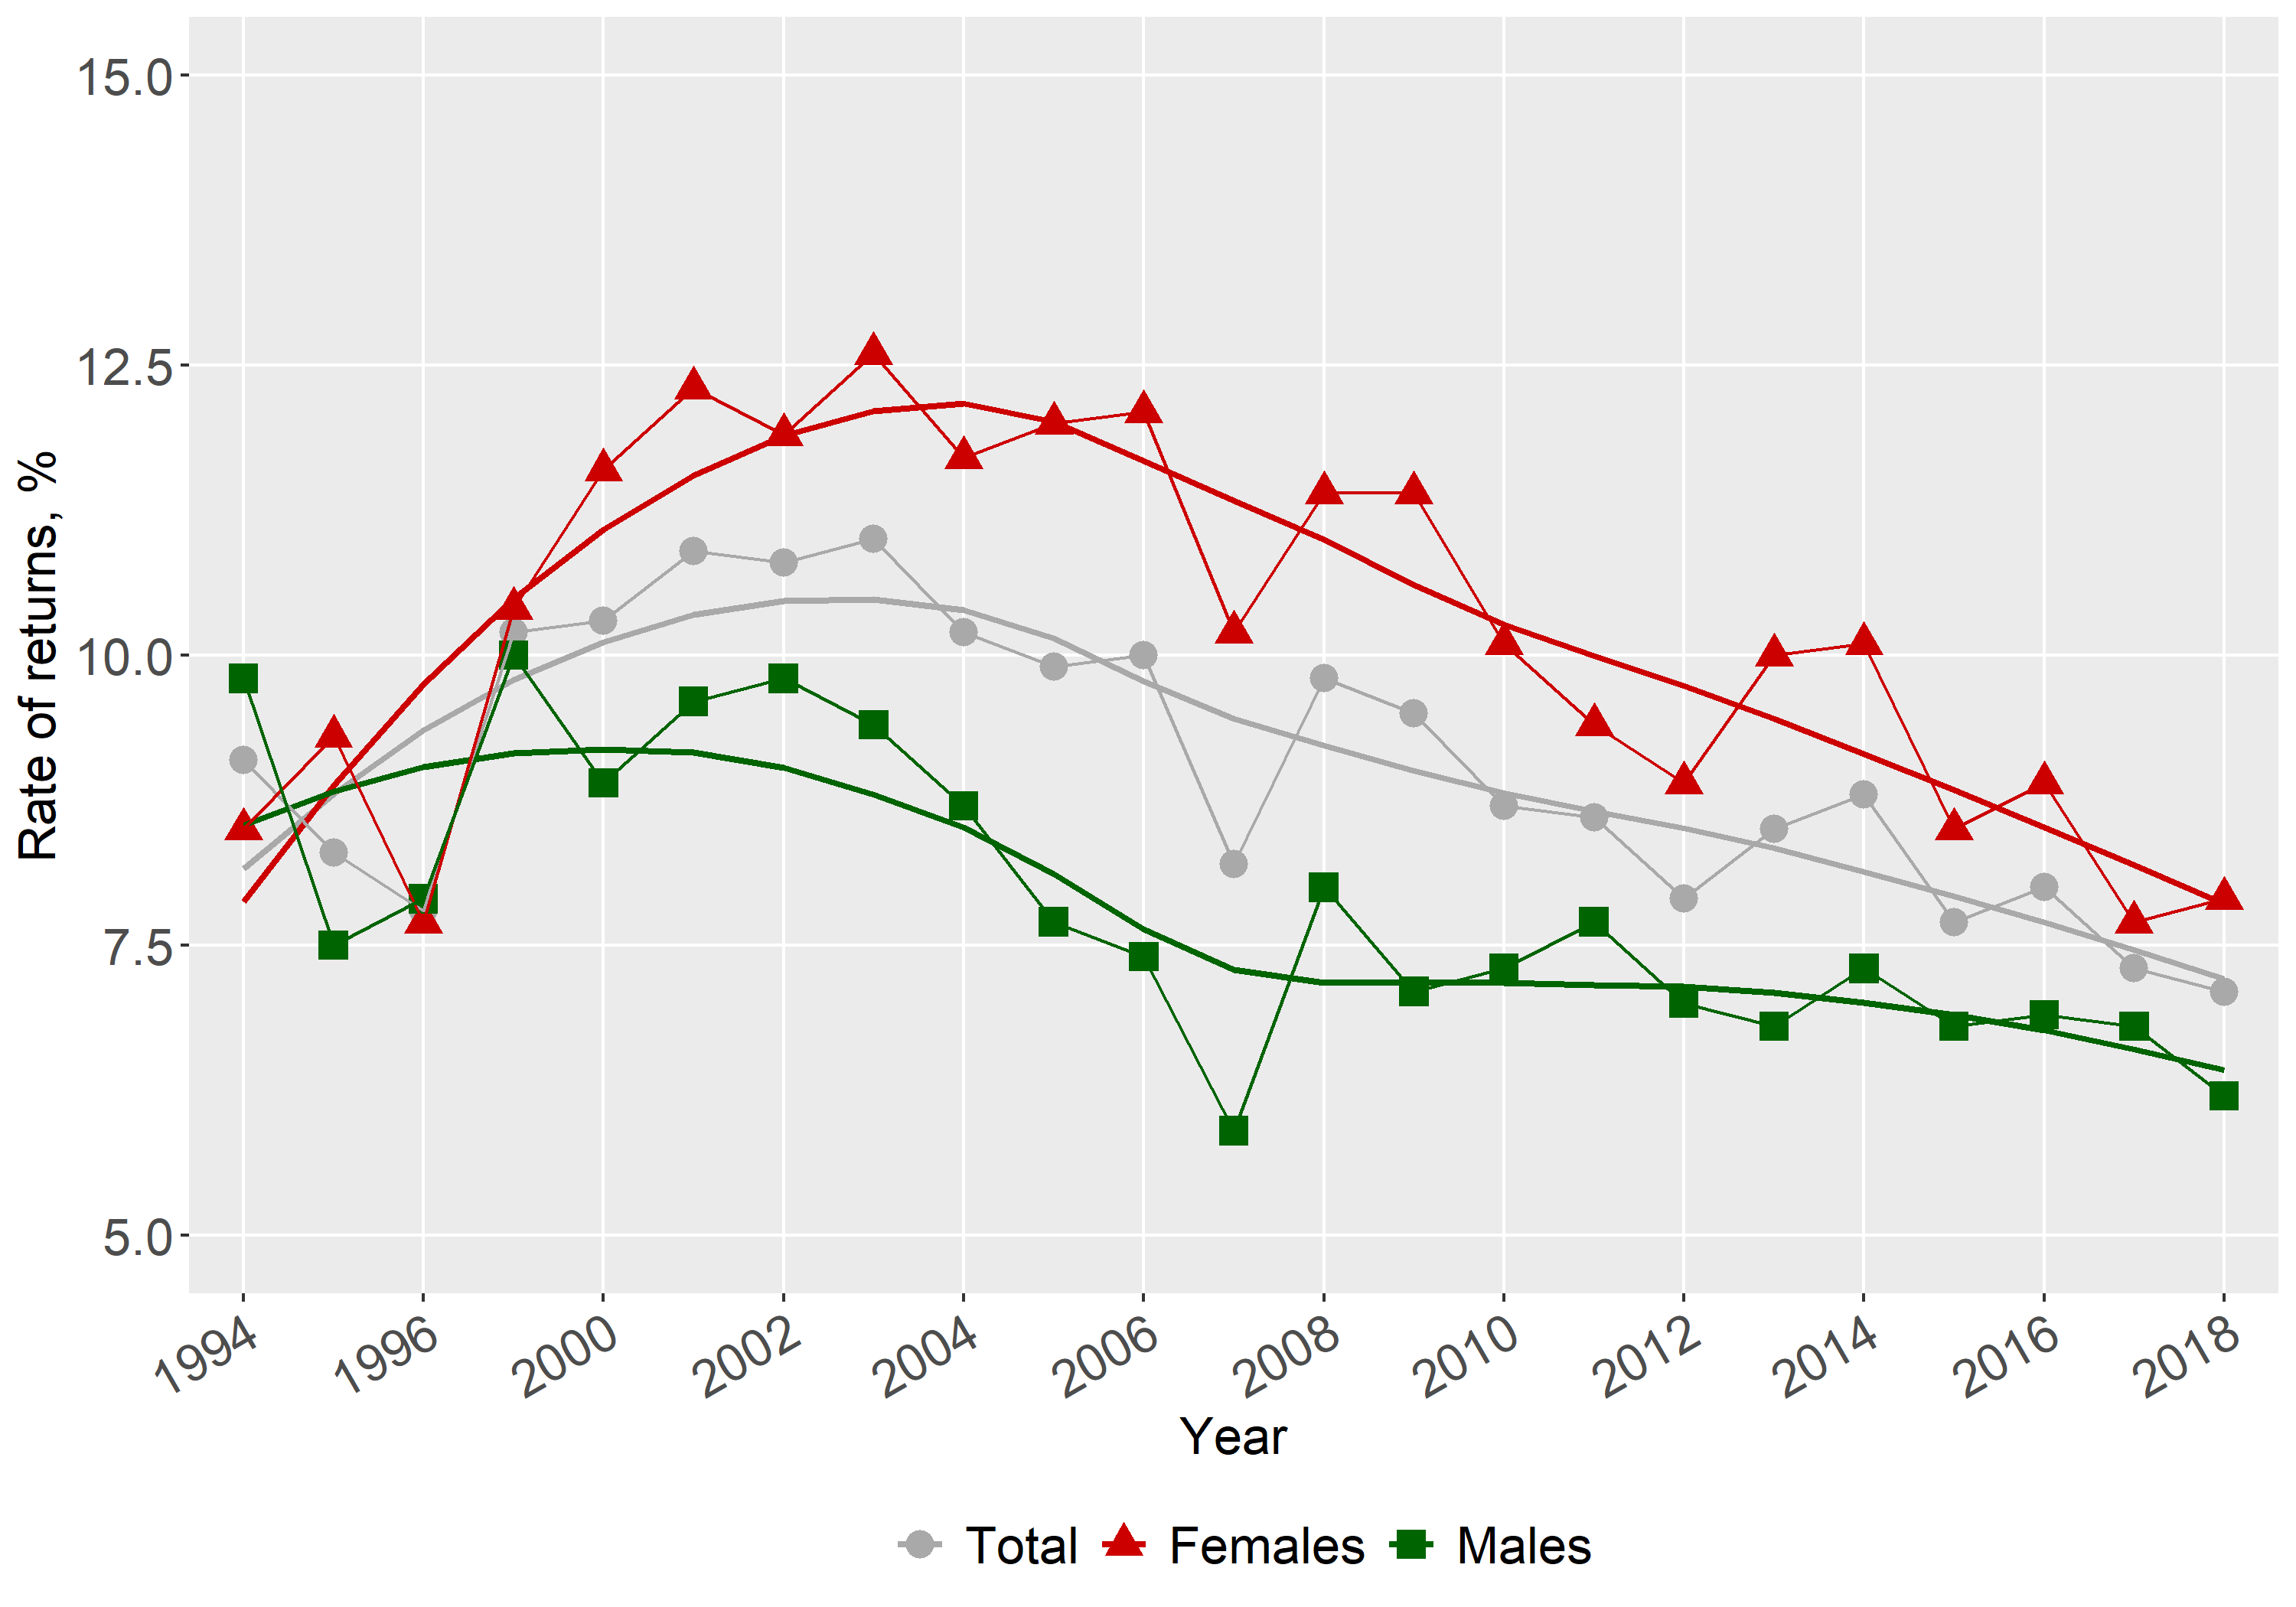
\includegraphics[width=\textwidth, height=300pt]{re_edu.png}
 \caption{Rates of Returns to Education in Russia, RLMS 1994-2018}\label{fig:1.1}
\end{figure}

We are particularly interested in the returns to specific levels of education, estimated through a series of dummy variables. Using Secondary Education completed as the base or omitted dummy for purpose of interpretation, we use dummies for Vocational Education and for Higher Education. The specification is presented in equation \eqref{eq:1.2}: 

\begin{flalign}\label{eq:1.2} 
Log(Wage) = a_0 + a_1\cdot D_{Voc} + a_2\cdot D_{Higher} + a_3\cdot Exp + a_4\cdot Exp^2 + a_5\cdot Gender + \epsilon
\end{flalign}




Figure \ref{fig:1.2}, panel (a) displays rates of returns to Higher and Vocational education (as compared to Secondary education) in Russia for the period 1994-2018. The results suggest that on average wage premiums to university education in Russia are roughly 3-5 times greater than to vocational schooling. The observed trend for premiums to both Vocational and Higher education levels is similar to the trend for education in general with the following peaks: 83\% for Higher education and 26\% for Vocational education compared to the average earnings of workers with a Secondary education. The interesting pattern to note from panel \ref{fig:1.2a} is the apparent co-movement of vocational education and higher education - the higher education smoothing curve turns a bit more sharply than the one for vocational education, but their movement is matching, even at second-order levels of smoothness. Further, even though higher education premium remains much above the premium for vocational education, there is a perceptible narrowing of the difference in recent years. Panel \ref{fig:1.2b}, which is drawn from a presentation made by Marina Telezhkina at the WB-HSE Summer School on the Economics of Education in July 2019, shows the interesting pattern of higher education enrollment rates for the population of 17-25 year old. Panel \ref{fig:1.2b} shows the downturn in returns reflected in enrollments, with the peak in enrollments coming about 10 years later. 

\begin{figure}[H]
\caption{\textbf{Rates of Returns to Higher and Vocational Education in Russia, RLMS 1994-2018}}\label{fig:1.2}
         \centering
         \begin{subfigure}[b]{0.5\textwidth}
                 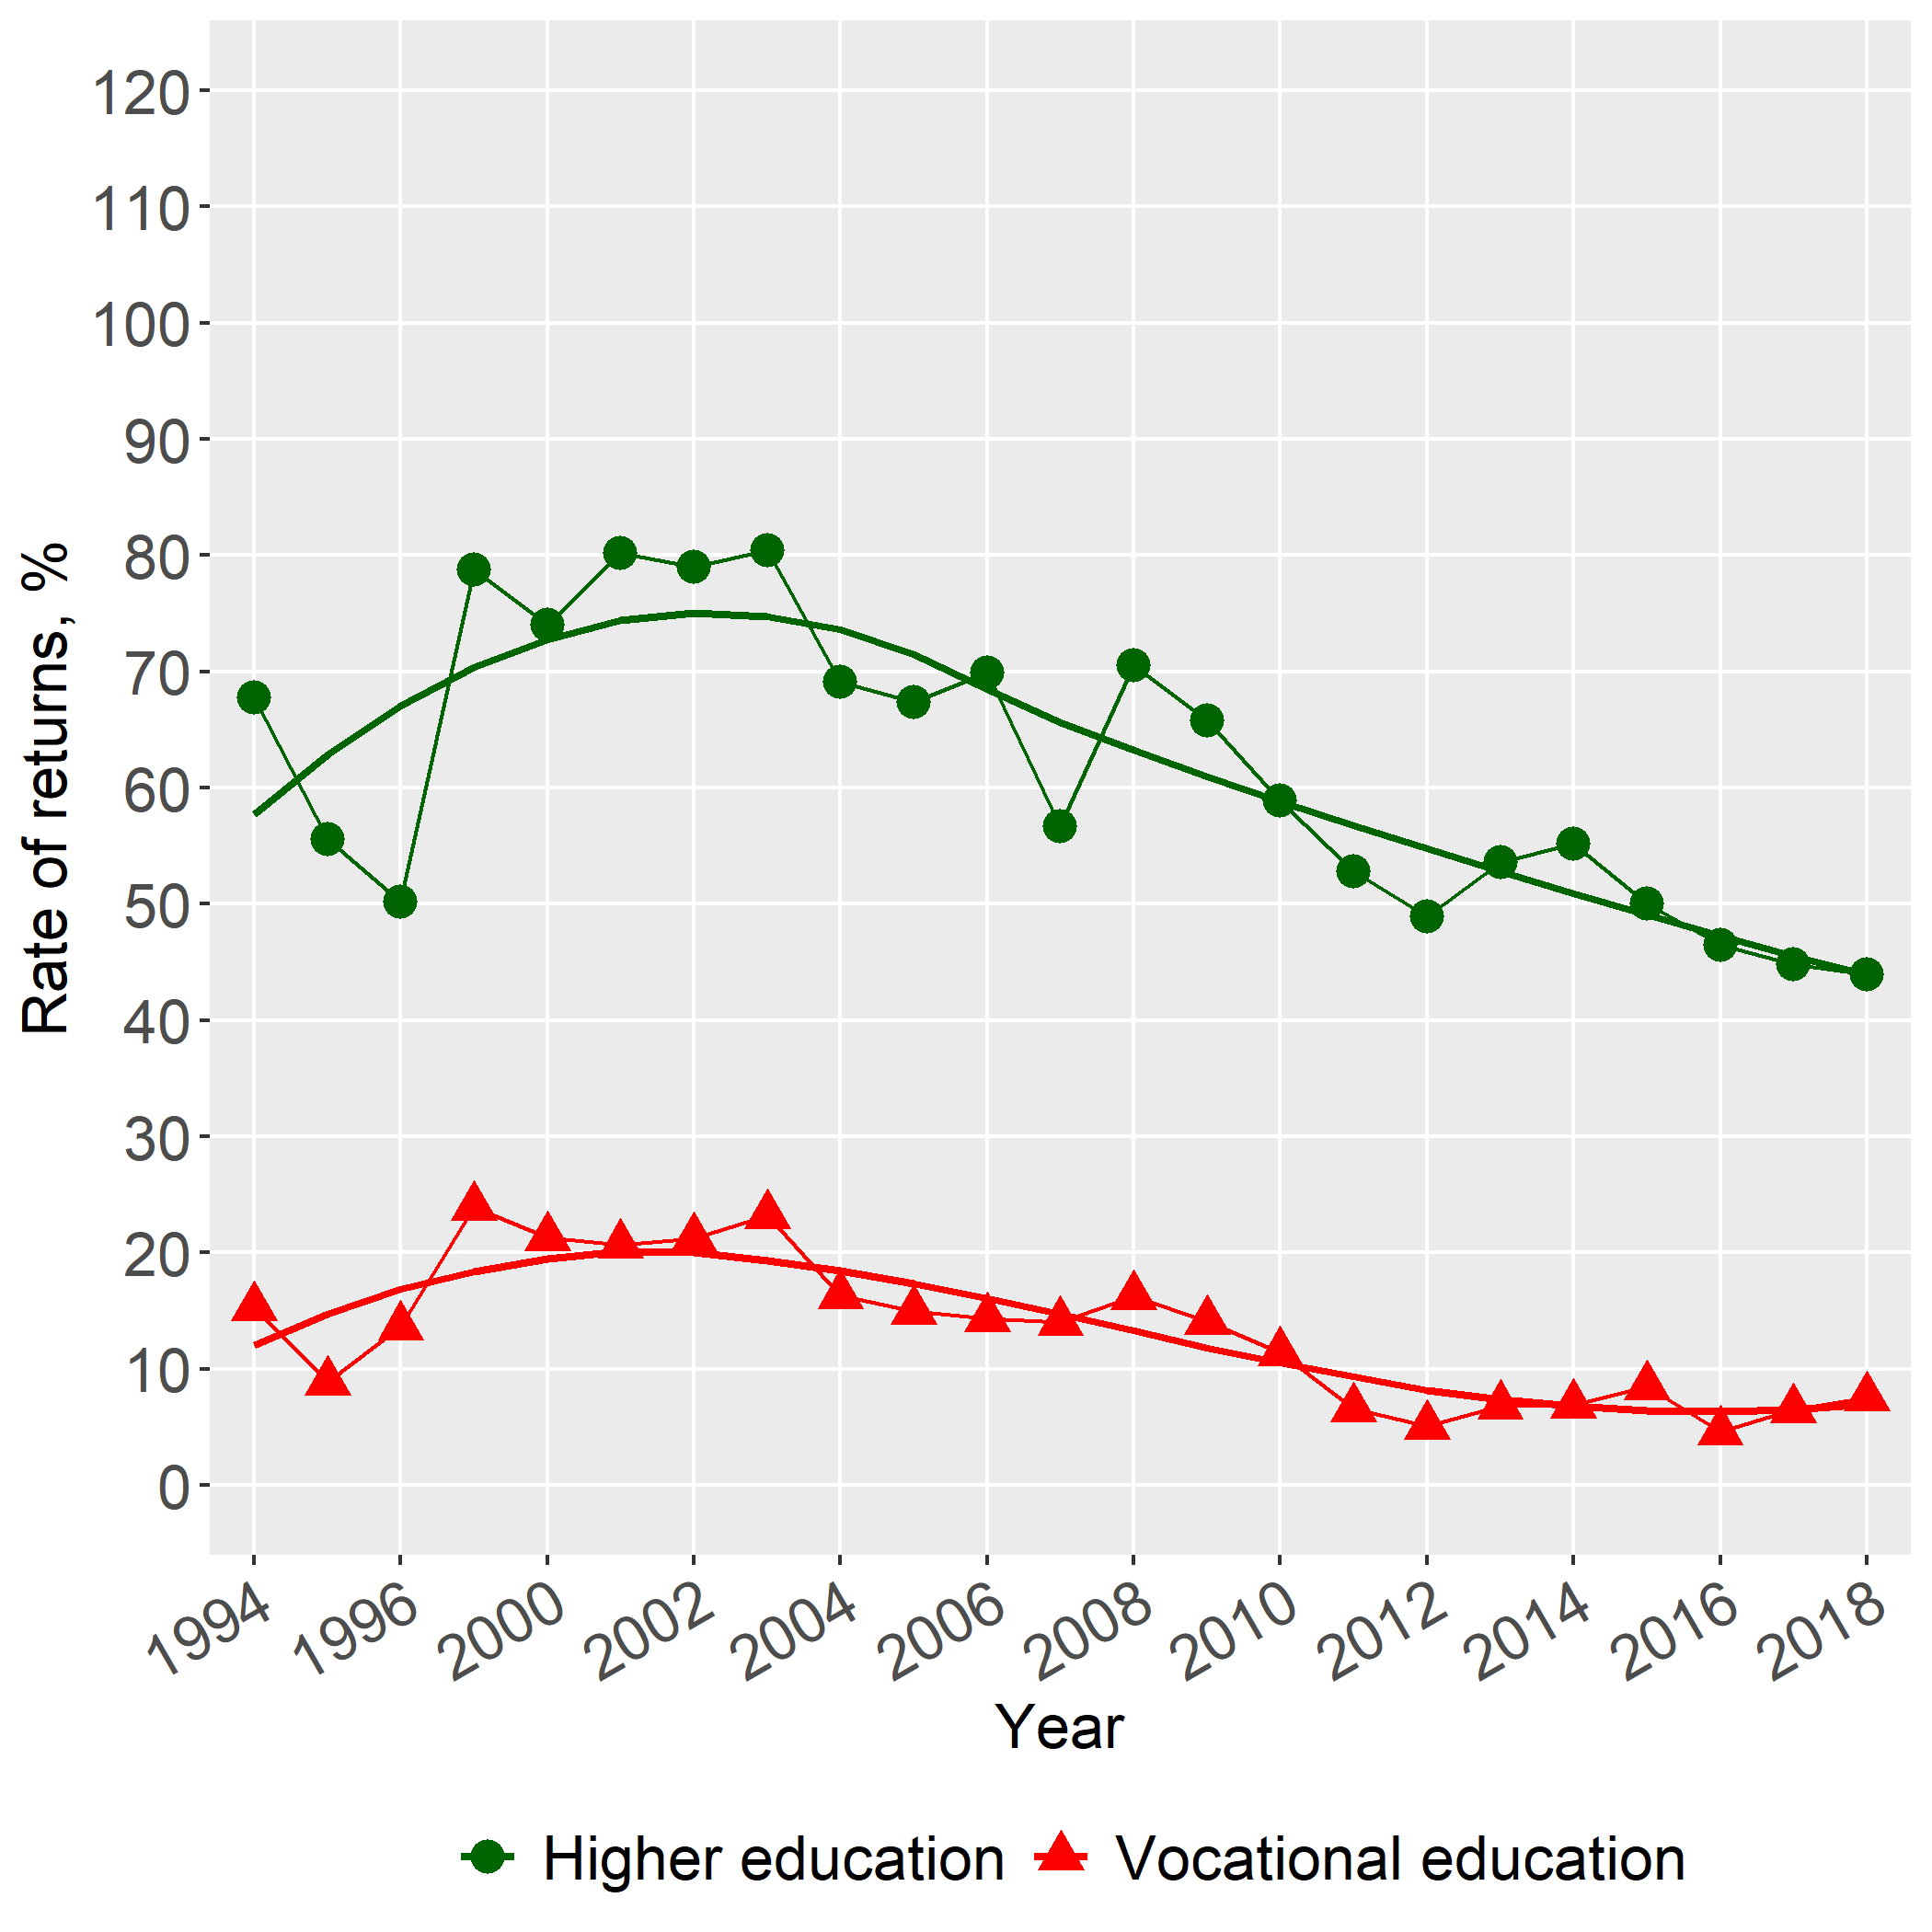
\includegraphics[width=\textwidth]{re_HE_all.png}
                 \caption{Rates of Return}
                 \label{fig:1.2a}
         \end{subfigure}%
         ~ %add desired spacing between images, e. g. ~, \quad, \qquad, \hfill etc.
           %(or a blank line to force the subfigure onto a new line)
         \begin{subfigure}[b]{0.5\textwidth}
                 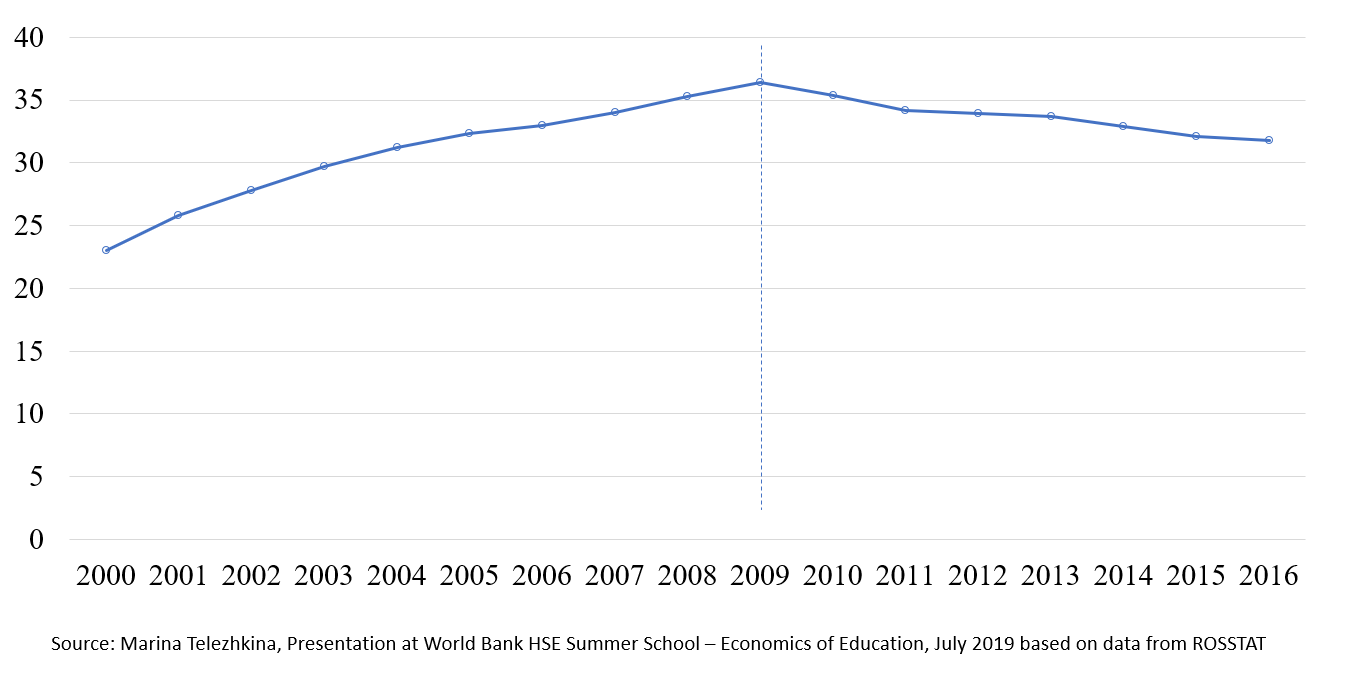
\includegraphics[width=\textwidth]{telezhkina.png}
                 \caption{Enrollment in Higher Education}
                 \label{fig:1.2b}
         \end{subfigure}
     \end{figure}

When estimated separately by gender, we find trend variation by gender. The results from estimation of earnings functions show that payoffs to Higher education for males varied from 45\% to 76\%, whereas women's returns are described by an inversely U-shaped pattern, reaching their maximum of 104\% in 2001. Within roughly the last 5 years, wage premiums to higher education for women have stabilized around the level of men (~50\%).  Gender wise enrollment rates in higher education (not shown) ten years later appears to match the differences in rates of return, strengthening the hypothesis that market rates of return to education in Russia do indeed influence individual continuing school decisions. 

A similar comparative picture is observed with respect to vocational education, albeit with a different kind of variation by gender (see Figure \ref{fig:1.3}): returns for males are almost flat within the time period while returns for females shows a concave pattern. The overall outcome concerning payoffs to schooling isolated by gender has been confirmed in a similar fashion by past studies \parencite[e.g.,][]{cheidvasser_006._2007}.

\begin{figure}[H]
  \begin{minipage}[b]{.5\linewidth}
     \centering
     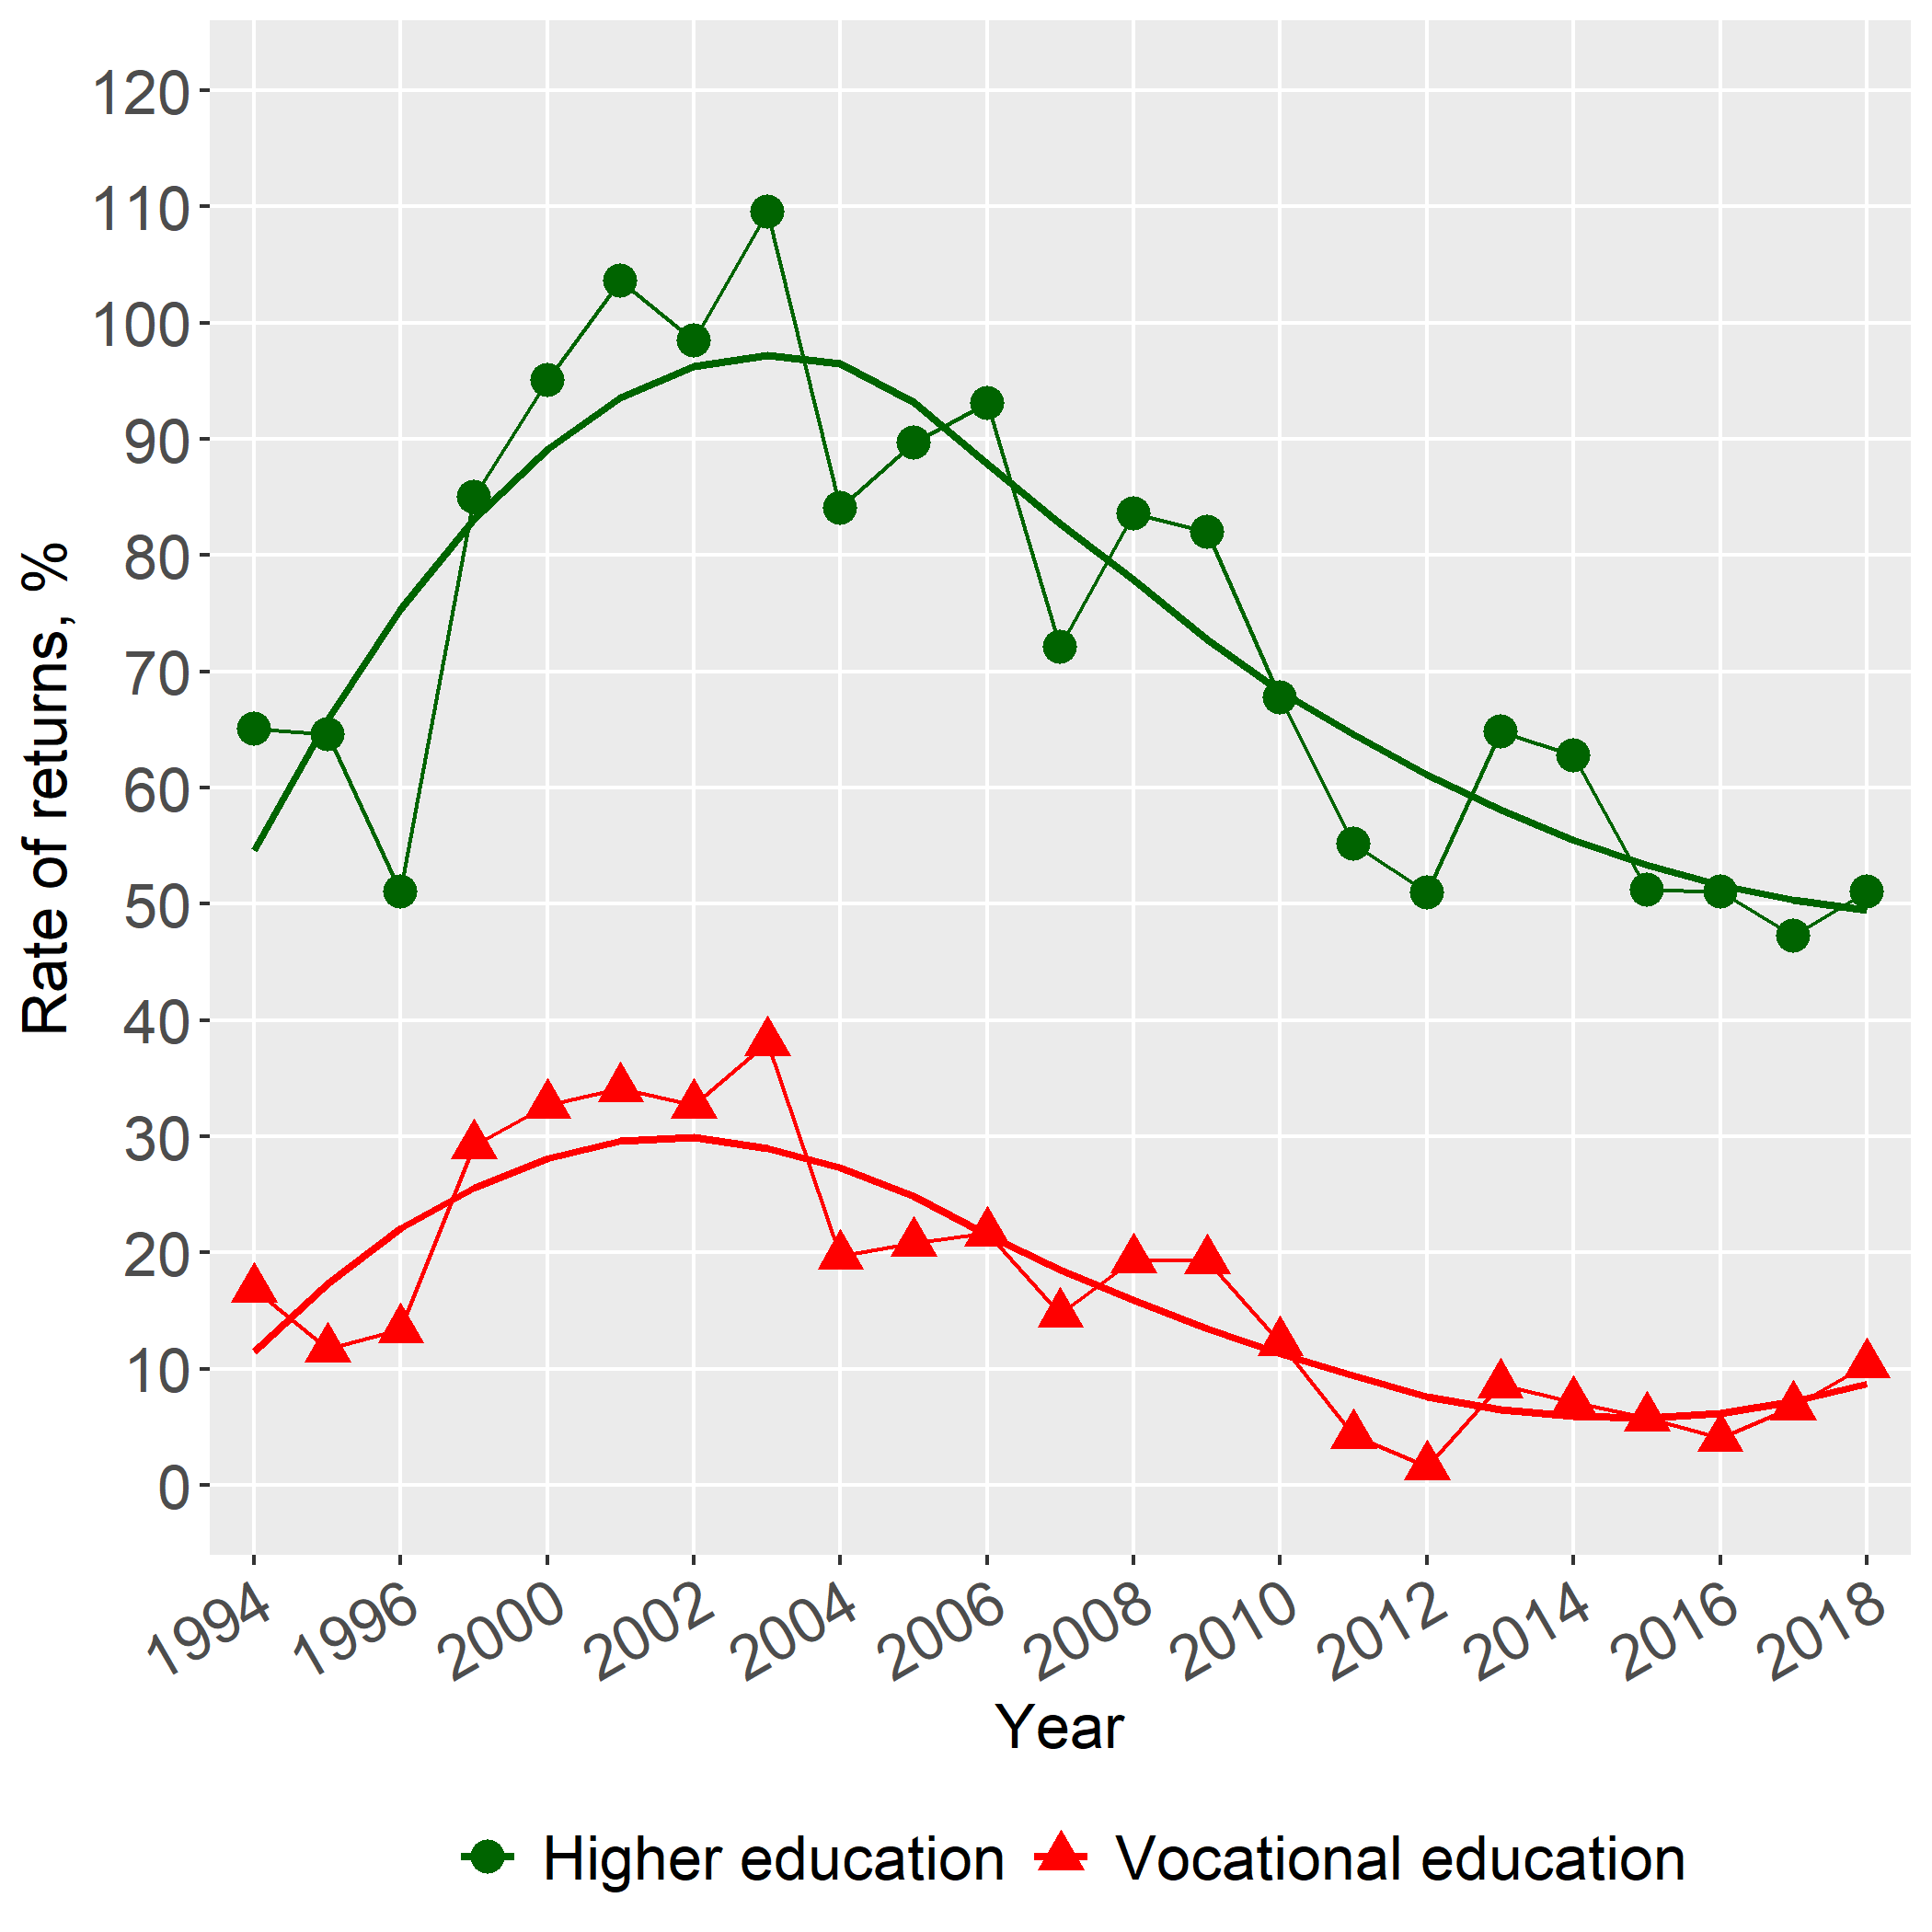
\includegraphics[width=\textwidth]{re_HE_f.png}
     % plot 1
     \subcaption{Females}\label{fig:1.3a}
  \end{minipage}
  \hfill
  \begin{minipage}[b]{.5\linewidth}
     \centering
     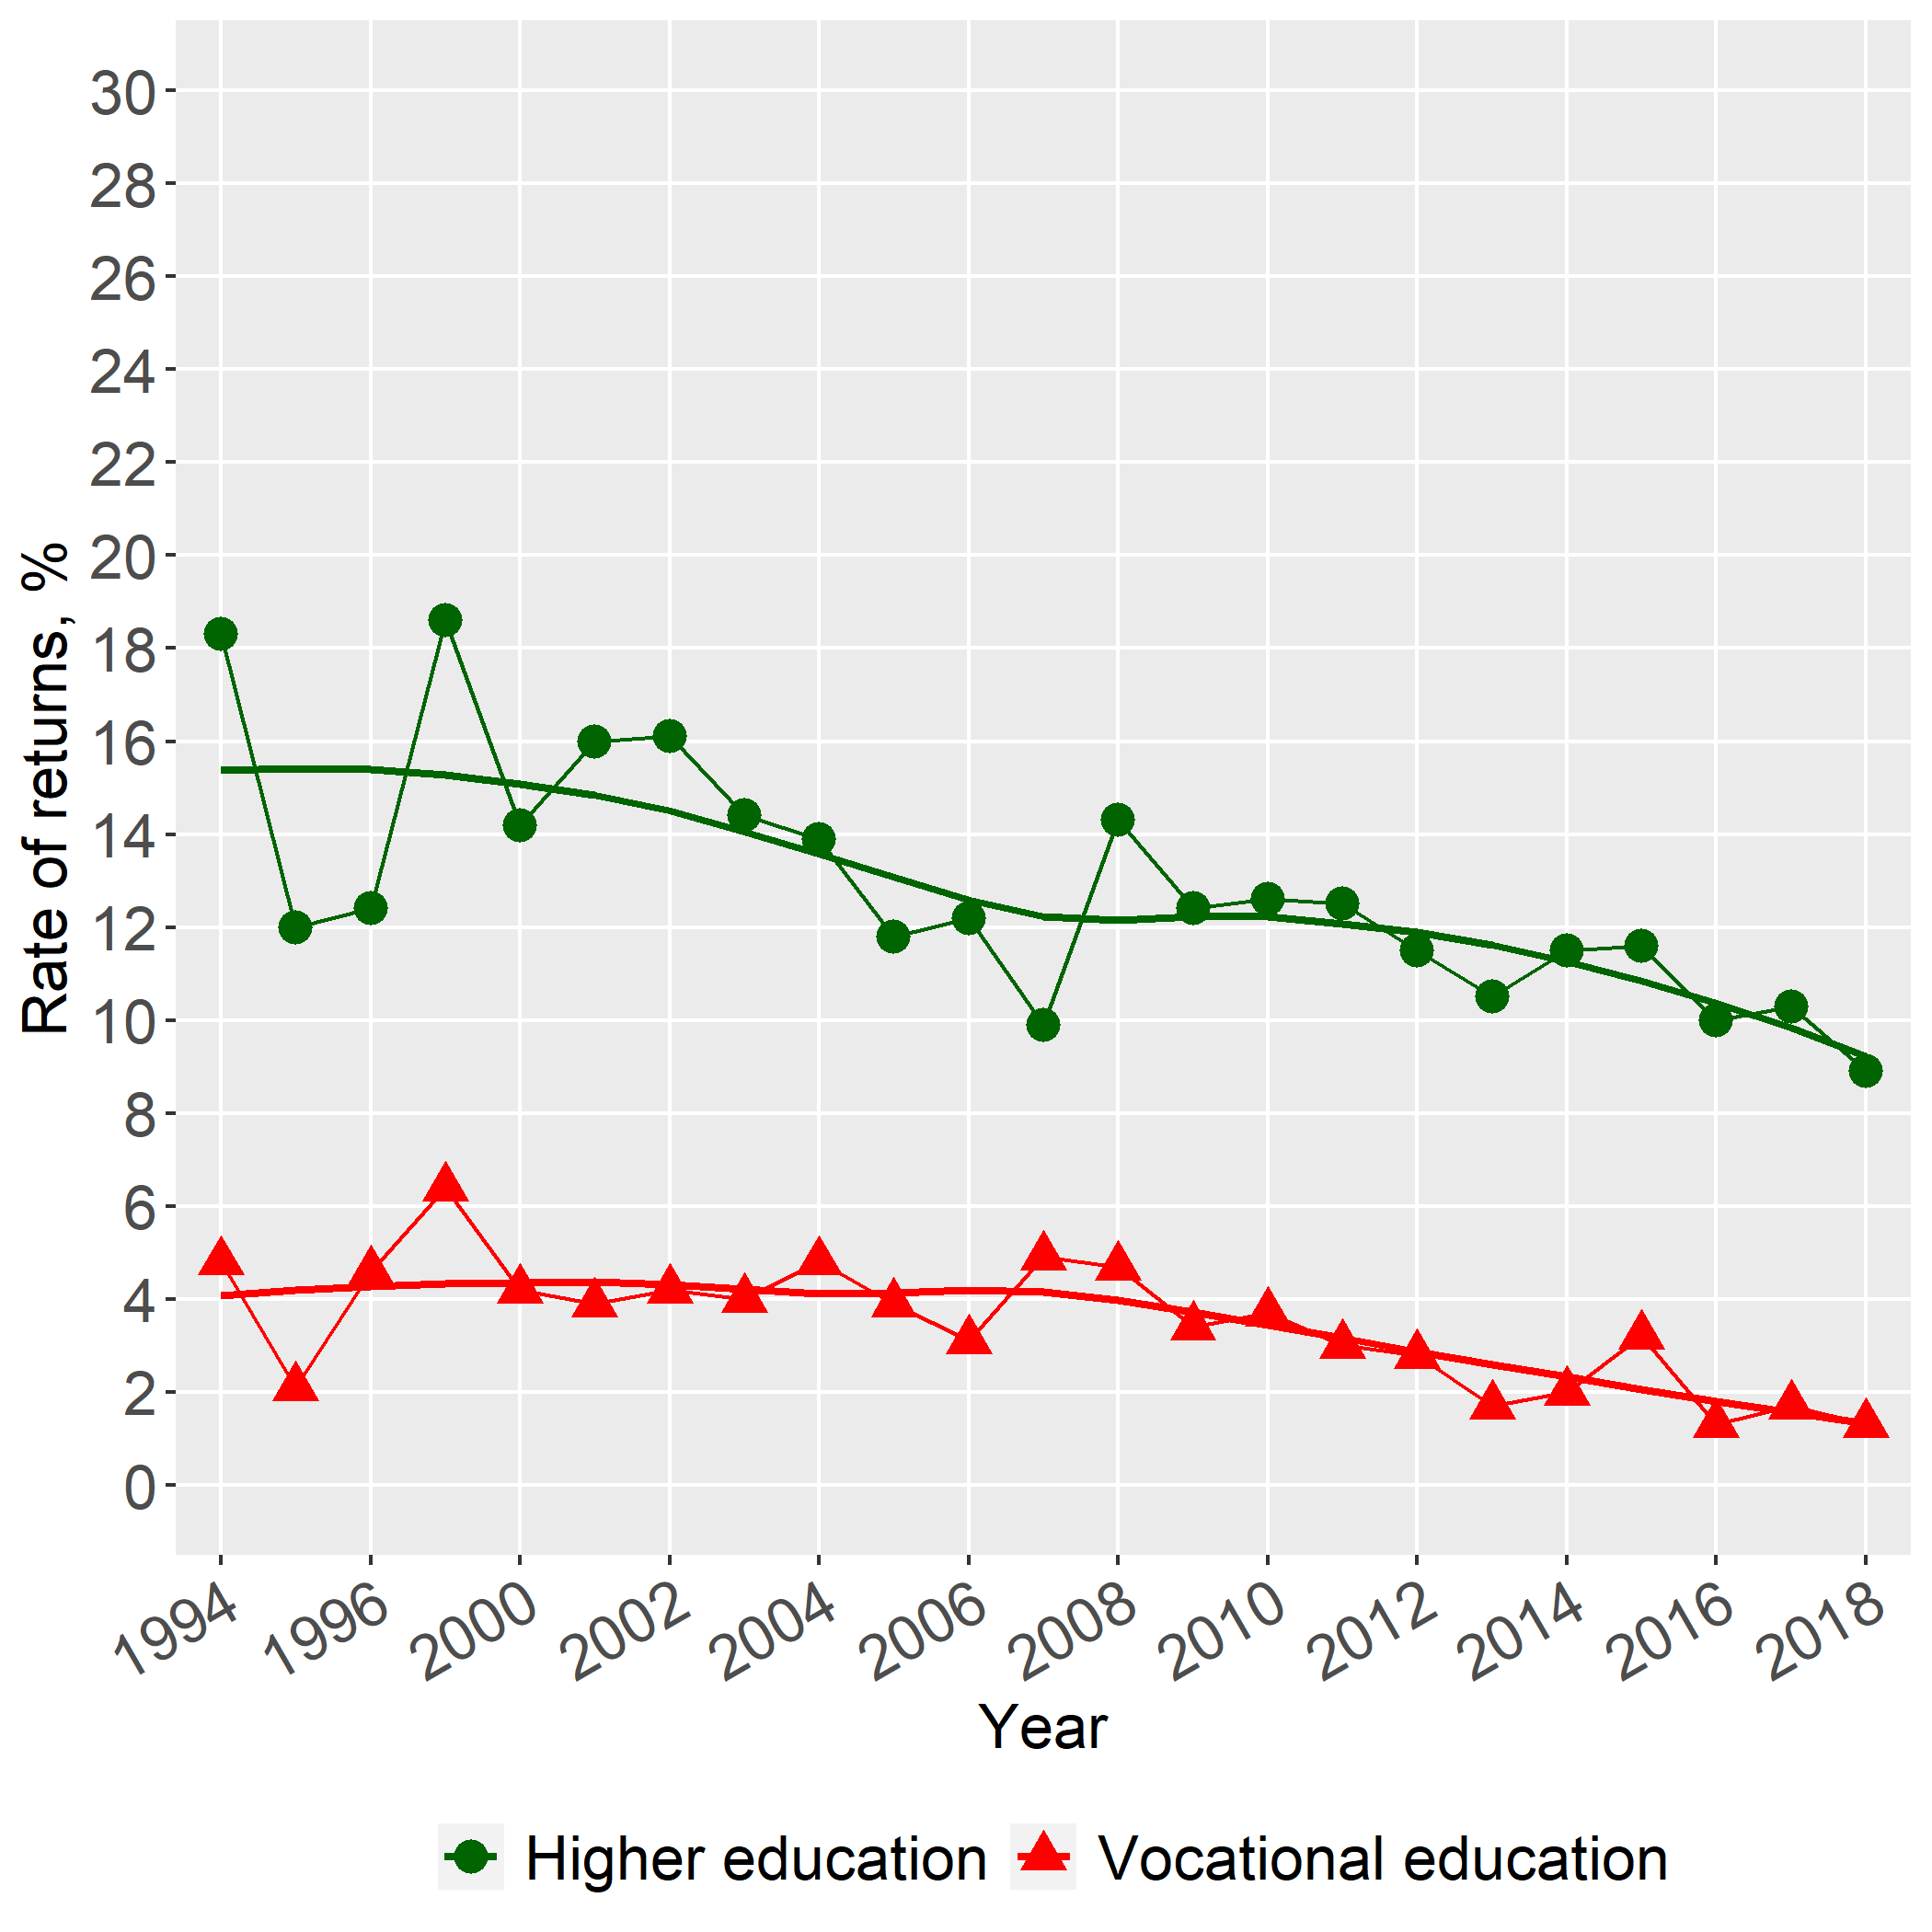
\includegraphics[width=\textwidth]{re_HE_m.png}
     % plot 2
     \subcaption{Males}\label{fig:1.3b}
  \end{minipage}
  \caption{Rates of Returns to Higher and Vocational Education in Russia, RLMS 1994-2018}\label{fig:1.3}
\end{figure}

%%%%%%%%%%%%%%%%%%%%%%%%%%%%%%%%%%%%%%%%%%%%%%%%%%%%%%%%

\section{Depreciation of Human Capital \\ in the Russian Federation}

Age-earnings profiles are almost invariably concave downward shaped. Earnings rise after a labor market entrant completes full-time schooling. The profile indicates a peak in earnings, usually a few years before retirement, after which there is a steady decline in earnings. The concave shape is an outcome of two countervailing tendencies - the rise attributed to continued accumulation of human capital through training and the decline due to depreciation. The precise shape and location of the peak is an object of analytical interest. Depreciation of human capital is useful to investigate from a policy perspective. Just like some physical capital (machinery, buildings) are built stronger and last longer, is it possible that some kinds of education inherently generate human capital that is slower to depreciate? What attributes of the labor market lead to lower or higher levels of depreciation? What about the welfare implications of changes in the age at which individuals retire from the labor force? How has the depreciation rate of human capital changed over time in the Russian Federation? In particular, can changes in the rate of depreciation explain the observed pattern of the rates of return depicted in \ref{fig:1.1}?  

\subsection{Analytical Treatment of Depreciation} 

\citet{rosen_176._1976}  and \citet{mincer_175._1982} presented early treatments on the depreciation of human capital. However, in terms of a focus on depreciation, a seminal paper of \citet{neuman_091._1995} established the basic parameters that have guided the research since that time. The authors introduce the important distinction between two kinds of depreciation or loss of productive potential of human capital. The first one, termed as ``obsolescence" or ``vintage effect", is due to an overall upgrading of technology or the operation of other market forces that lowers the value of education or training obtained in a previous period. This is also termed as an `external depreciation", presumably as it is a given for an individual. The second kind of depreciation is attributed to the deterioration of physical and mental abilities of an individual due to the progression of a person's age, or the simple passage of time. This is also termed as ``internal depreciation". Neuman and Weiss posited that external effects would be more important for higher levels of education, under the assumption that changes in the labor market are transmitted more readily to higher education. They give the example that a recently educated electrical engineer would be learning many new things compared to one who studied the same subject in an earlier time. Neuman and Weiss reasoned that workers with basic education levels may not suffer as much from obsolescence. 

Figure \ref{fig:2.1} shows for the Russian Federation the effects described by Neuman and Weiss. There are three panels in the figure, and three lines in each figure. The vertical axis indicates the monthly earnings in constant 2018 rubles, using the Rosstat CPI deflator. The horizontal axis indicates the years of experience. The dotted line shows the earnings for 1998, the dashed line represents 2006 and the solid line the data from 2018. Each of the panels, representing a different level of education, shows an upward drift in the experience-earnings profiles in the period from 1998 to 2018. Only Figure \ref{fig:2.1a} shows a clear concave downwards profile for Higher Education; the concave tendency is less pronounced for the other two levels of Vocational education and Secondary education.
	
	\begin{figure}[H]
		\begin{minipage}[b]{.3\linewidth}
			\centering
			\hspace*{-0.7in}
			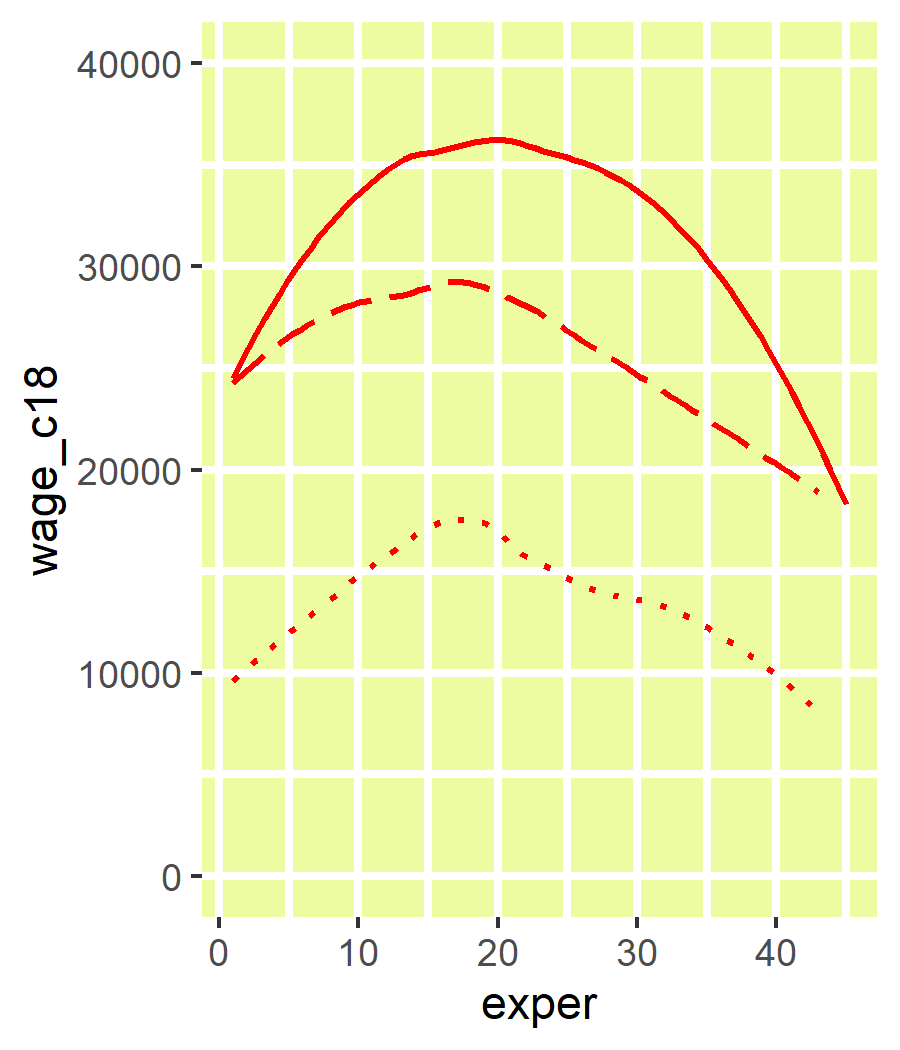
\includegraphics[width=150pt]{dp01_he.png}
			% plot 1
			\subcaption{Higher Education}\label{fig:2.1a}
		\end{minipage}
		\hfill
		\begin{minipage}[b]{.3\linewidth}
			\centering
			\hspace*{-0.7in}
			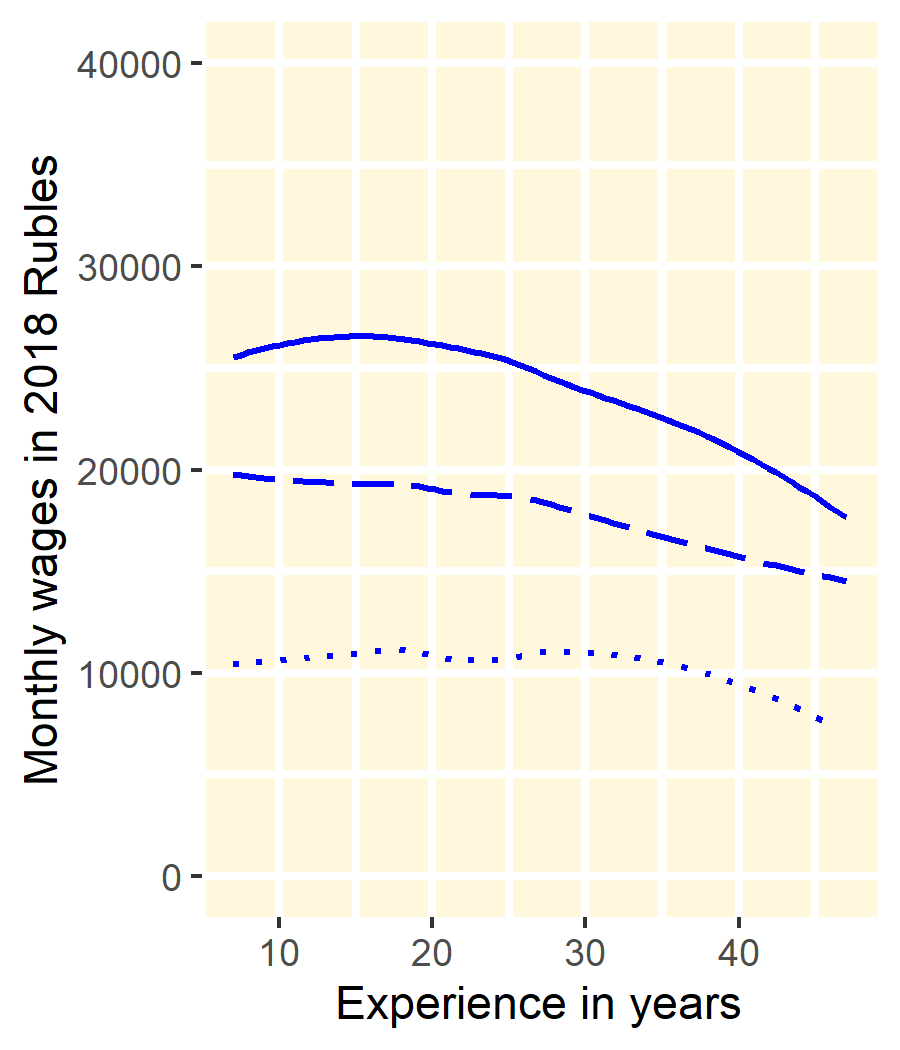
\includegraphics[width=150pt]{dp01_ve.png}
			% plot 2
			\subcaption{Vocational Education}\label{fig:2.1b}
		\end{minipage}
		\hfill
		\begin{minipage}[b]{.3\linewidth}
			\centering
			\hspace*{-0.7in}
			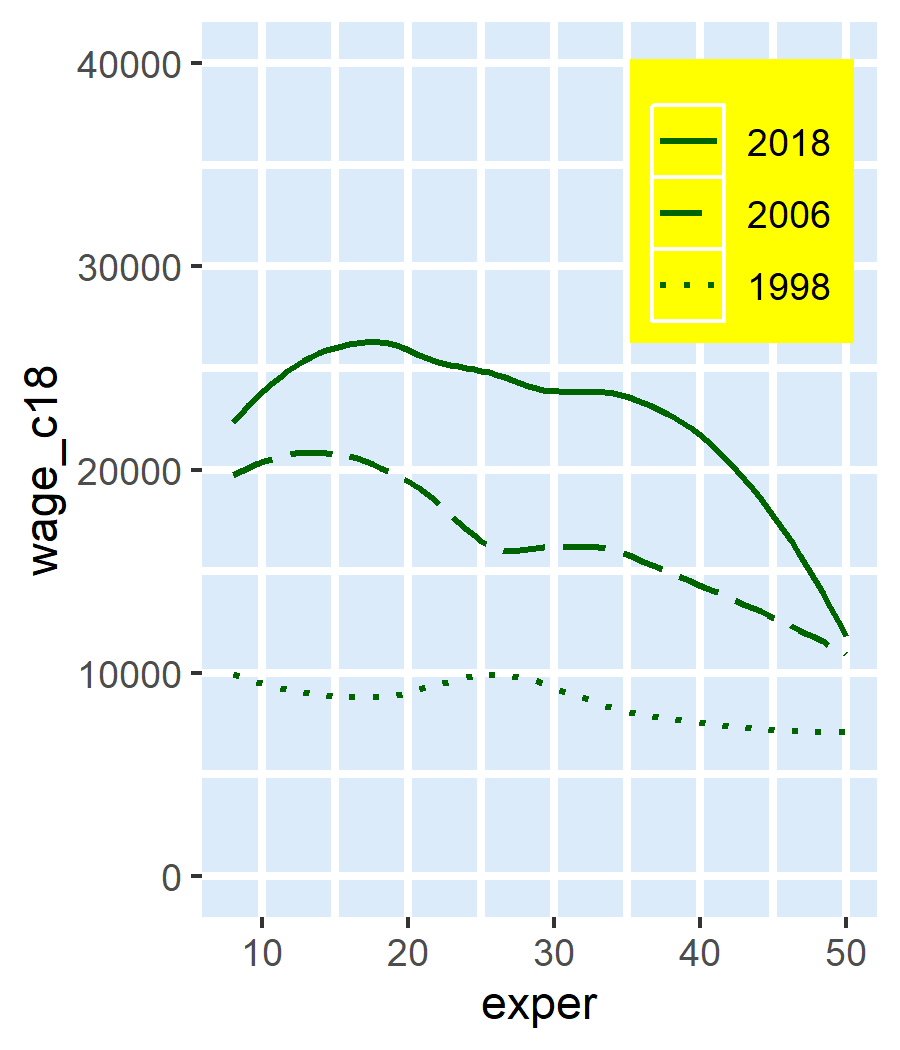
\includegraphics[width=150pt]{dp01_se.png}
			% plot 2
			\subcaption{Secondary Education}\label{fig:2.1c}
		\end{minipage}
		\caption{Neuman-Weiss vintage effects by education level from RLMS Rounds 1998, 2006 and 2018}\label{fig:2.1}
	\end{figure}
	
Putting the curves together by year (Figure \ref{fig:2.2})suggests that the premium for university education over the other two levels does narrow at higher levels of experience. In the figure, to accomodate the relatively lower wage levels of 1998, the leftmost panel (Figure \ref{fig:2.2a}) is slightly compressed compared to the other two panels. The  converging tendency between levels of education would suggest that depreciation is indeed higher for university graduates. In the next two subsections, we present a more rigorous quantitative treatment of this issue, using a variant of Neuman-Weiss developed by \citet{murillo_172._2006}.

	
	\begin{figure}[H]
		\begin{minipage}[b]{.3\linewidth}
			\centering
			\hspace*{-0.7in}
			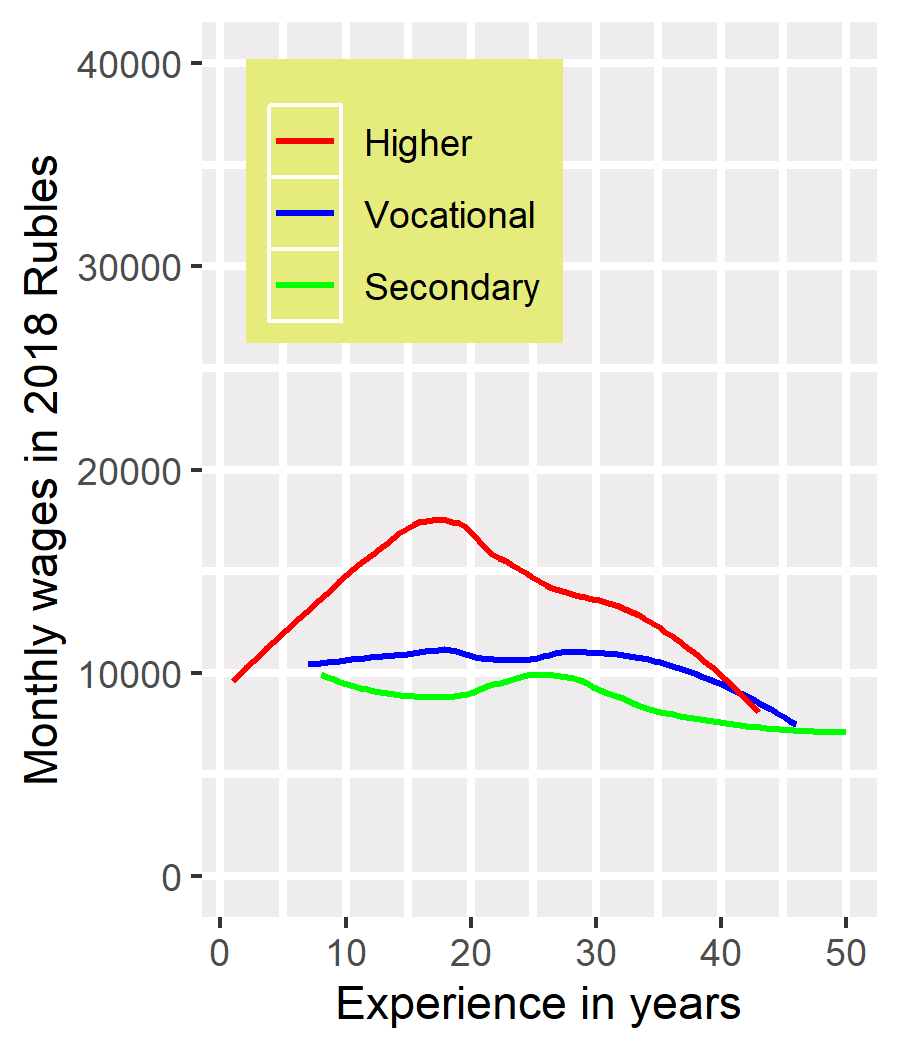
\includegraphics[width=150pt]{dp01_98.png}
			% plot 1
			\subcaption{1998}\label{fig:2.2a}
		\end{minipage}
		\hfill
		\begin{minipage}[b]{.3\linewidth}
			\centering
			\hspace*{-0.7in}
			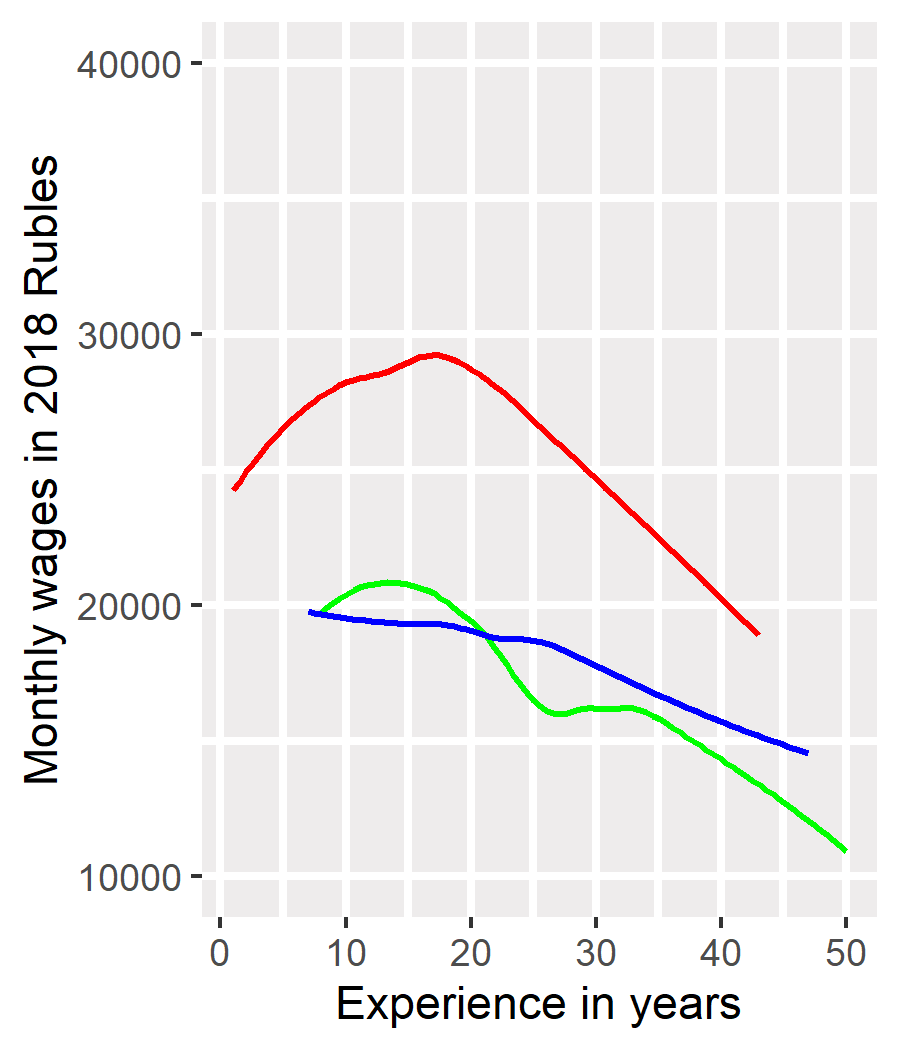
\includegraphics[width=150pt]{dp01_06.png}
			% plot 2
			\subcaption{2006}\label{fig:2.2b}
		\end{minipage}
		\hfill
		\begin{minipage}[b]{.3\linewidth}
			\centering
			\hspace*{-0.7in}
			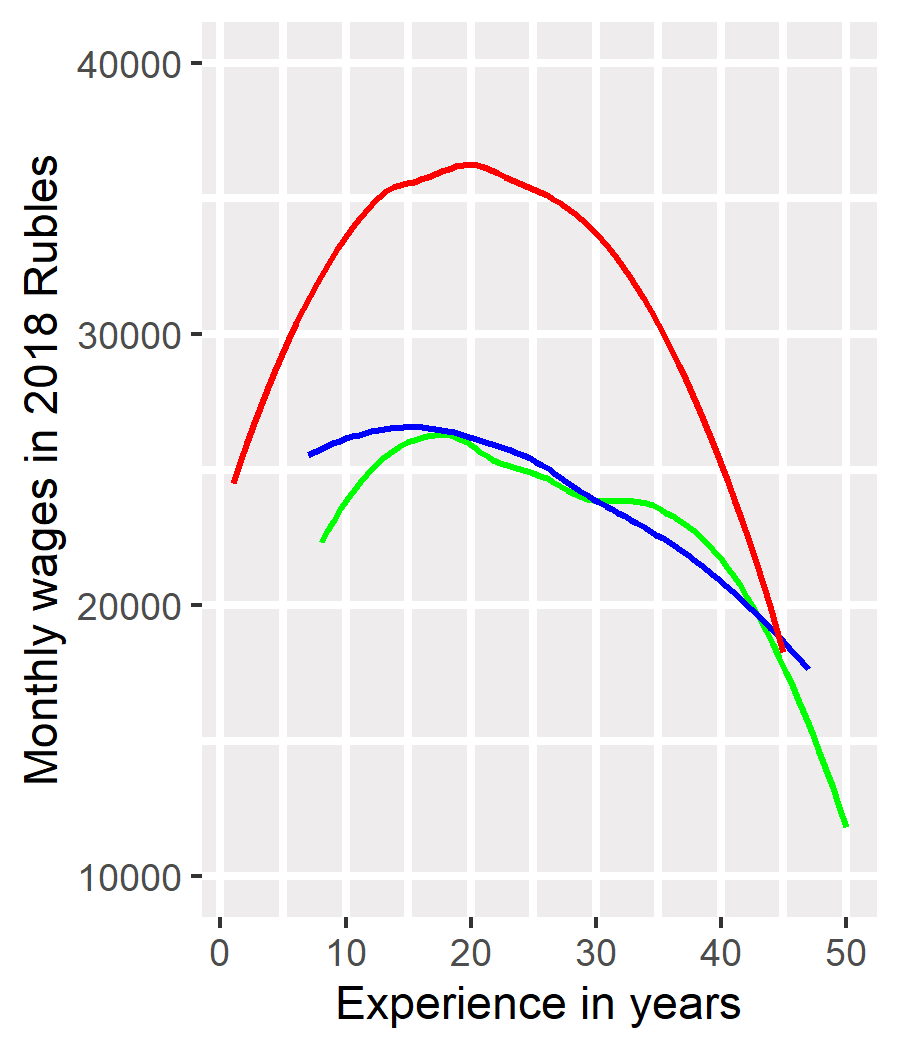
\includegraphics[width=150pt]{dp01_18.png}
			% plot 2
			\subcaption{2018}\label{fig:2.2c}
		\end{minipage}
		\caption{Neuman-Weiss vintage effects by Year from RLMS Rounds 1998, 2006 and 2018}\label{fig:2.2}
	\end{figure}

\subsection{Differential Depreciation Affecting Education and Training}
	
\citet{murillo_172._2006} implemented a variation of the Neuman and Weiss model with a focus on empirical implementation to Spain. We follow the Murillo notation in the implementation of the model, which begins with the following earnings equation: 
\begin{flalign}\label{eq:2.1} 
log(W_{T}) = \alpha + \beta_{1}KS_{T} +  \beta_{2}KE_{T} &&
\end{flalign}
\noindent
where $W$ represents earnings, $KS$ the stock of human capital derived from schooling of $S$ years, and $KE$ the stock of human capital acquired from on the job training or experience, and $T$ indexes the number of experience years since completing formal education. In this set-up, the parameters $\beta_1$ and $\beta_2$ are the productivity parameters for the respective parts of the stock of human capital. Both are assumed to suffer from depreciation or the loss of productive value. At this stage, we do not distinguish between the causes (internal or external) of this loss. The path of the stock of human capital due to education is given by 
\begin{flalign}\label{eq:2.2} 
KS_{T} = S + hTS &&
\end{flalign} 
\noindent
where $h$ is the rate of loss of the stock. The next equation for the loss of stock gained from experience is a bit more complicated. The stock from schooling, $S$ is taken to be fixed at the end of the full-time schooling period and the beginning of the working period. However, experience is being built up every year at the same time as the capital acquired from previous experience depreciates. 
\begin{flalign}\label{eq:2.3} 
KE_{T} = \{1 + (T-1)\cdot\gamma \} + \{1 + (T-2)\cdot\gamma \}  + \{1 + (T-3)\cdot\gamma \} + \ldots + \{1\}  && 
\end{flalign} 
\noindent
where $\gamma$ is the rate of loss applied every year. The equation can be simplified and summarized as
\begin{flalign}\label{eq:2.4} 
KE_{T} =  T + \gamma\cdot\{(T-1) + (T-2) + (T-3) + \ldots + 1\} = T + \gamma\cdot\frac{T^2}{2}   && 
\end{flalign} 
Substituting equations \ref{eq:2.2} and \ref{eq:2.4} into equation \ref{eq:2.1}, we get
\begin{flalign}\label{eq:2.5} 
log(W) = \alpha +  \beta_{1}S +  \beta_{1}hTS + \beta_{2}T + \frac{\beta_{2}\gamma}{2}T^{2} =  \alpha +  \beta_{1}S + \pi_{1}TS + \beta_{2}T + \pi_{2}T^{2} && 
\end{flalign} 
\noindent
where $\pi_{1} = \beta_{1}h$ and $\pi_{2} = \frac{\beta_{2}\gamma}{2}$. 
\vspace{2pt}
\noindent
From \ref{eq:2.5}, the depreciation rate during $T$ years applied to schooling can be computed as $\pi_{1}S $ and the depreciation rate applied to experience as $ 2\pi_{2}T$.
\vspace{-5pt}
\subsubsection{Estimation Results}
Table \ref{tab:2.1} shows OLS estimation results of equation \ref{eq:2.5} run on the whole sample of the RLMS observations. In this subsection, we analyzed separately six years that represent the ends (1994 and 2018), the diffused peak (2003 and 2006), and halfway points to the ends (2012 and 2003) of the available time interval. The idea is to examine the role played by changes in depreciation to explain the observed pattern of variation in the rates of return shown in Figure \ref{fig:1.1}. 

\setlength{\tabcolsep}{2pt}
\begin{table}[h!]
	\centering 
	\caption{Results of Estimating Human Capital Depreciation for the Whole Sample, RLMS} 
	\label{tab:2.1}
	\begin{tabular}{@{\extracolsep{3pt}}lcccccc} 
		\\[-1.8ex]\hline 
		\hline \\[-1.8ex] 
		& \textbf{1994} & \textbf{1998} & \textbf{2003} & \textbf{2006} & \textbf{2012} & \textbf{2018} \\ 
		\\[-1.8ex] & (1) & (2) & (3) & (4) & (5) & (6)\\ 
		\hline \\[-1.8ex] 
		Constant & 10.266$^{***}$ & 4.720$^{***}$ & 6.762$^{***}$ & 7.854$^{***}$ & 8.889$^{***}$ & 9.205$^{***}$ \\ 
		& (0.301) & (0.258) & (0.221) & (0.181) & (0.128) & (0.158) \\ 
		& & & & & & \\ 
		Educ, years ($S$) & 0.113$^{***}$ & 0.116$^{***}$ & 0.094$^{***}$ & 0.074$^{***}$ & 0.054$^{***}$ & 0.053$^{***}$ \\ 
		& (0.020) & (0.017) & (0.015) & (0.012) & (0.008) & (0.010) \\ 
		& & & & & & \\ 
		Educ X Exper ($TS$) & $-$0.001$^{*}$ & $-$0.001$^{*}$ & $-$0.00005 & 0.0003 & 0.0003 & 0.0001 \\ 
		& (0.001) & (0.001) & (0.001) & (0.0005) & (0.0003) & (0.0004) \\ 
		& & & & & & \\ 
		Exper($T$) & 0.053$^{***}$ & 0.044$^{***}$ & 0.016 & $-$0.001 & 0.012$^{*}$ & 0.023$^{***}$ \\ 
		& (0.015) & (0.013) & (0.011) & (0.009) & (0.007) & (0.008) \\ 
		& & & & & & \\ 
		Exper squared ($T^2$) & $-$0.001$^{***}$ & $-$0.001$^{***}$ & $-$0.0004$^{***}$ & $-$0.0002$^{*}$ & $-$0.001$^{***}$ & $-$0.001$^{***}$ \\ 
		& (0.0002) & (0.0001) & (0.0001) & (0.0001) & (0.0001) & (0.0001) \\ 
		& & & & & & \\ 
		\hline \\[-1.8ex] 
		Observations & 3,037 & 3,100 & 3,856 & 4,800 & 7,417 & 6,112 \\ 
		R$^{2}$ & 0.043 & 0.058 & 0.068 & 0.078 & 0.088 & 0.071 \\ 
		Adjusted R$^{2}$ & 0.042 & 0.057 & 0.067 & 0.077 & 0.087 & 0.071 \\ 
		Residual Std. Error & 0.934 & 0.800 & 0.782 & 0.715 & 0.666 & 0.617 \\ 
		F Statistic & 34.062$^{***}$ & 47.678$^{***}$ & 69.846$^{***}$ & 101.053$^{***}$ & 177.952$^{***}$ & 117.104$^{***}$ \\ 
		\hline 
		\hline \\[-1.8ex] 
		\textit{Note:}  & \multicolumn{6}{r}{$^{*}$p$<$0.1; $^{**}$p$<$0.05; $^{***}$p$<$0.01} \\ 
	\end{tabular} 
\end{table}


Using the coefficient estimates derived from Table \ref{tab:2.1}, we compute the depreciation rate during $T$ years applied to schooling as $\pi_{1}S $ and the depreciation rate applied to experience as $ 2\pi_{2}T$, evaluating the expression at the mean level of schooling. Table \ref{tab:2.2} reports the depreciation rate values so calculated with the corresponding sample means. The table shows an interesting U-shaped pattern in the depreciation rate for human capital. The depreciation rate associated with education has been declining steadily and did not pick up again as measured with the given data. The depreciation rate associated with experience declined at first and then picked up again. 

\begin{table}[h!]
	\centering
	\caption{Average Depreciation Rates (DR) by Years, RLMS}
	\label{tab:2.2}
	\begin{tabular}{@{\extracolsep{20pt}}rlrrrrrr}
		\hline
		& \textbf{Statistic} & \textbf{1994} & \textbf{1998} & \textbf{2003} & \textbf{2006} & \textbf{2012} & \textbf{2018} \\ 
		\hline
		1 & Experience, mean & 12.70 & 12.69 & 12.79 & 12.79 & 12.95 & 13.27 \\ 
		2 & Education, mean & 21.41 & 22.32 & 22.20 & 22.24 & 22.52 & 22.52 \\ 
		\midrule
		3 & DR Experience, \% & 1.87 & 1.55 & 1.04 & 0.50 & 1.37 & 1.63 \\ 
		4 & DR Education, \% & 2.80 & 2.71 & 0.11 & 0.00 & 0.00 & 0.00 \\ 
		5 & DR Human Capital, \% & 4.67 & 4.26 & 1.15 & 0.50 & 1.37 & 1.63 \\ 
		\hline
	\end{tabular}
\end{table}
	
Further work is required, including computation of the depreciation rates at levels other than the mean values. At this stage, the findings raise some interesting questions which needs to be addressed by further research. In the period from 1994 to 2006, the depreciation rate appears to be declining, just as the rates of return were on an ascending curve. As both kinds of depreciation (for experience and education) were declining, it is possible that the main cause was in the labor market experience rather than in the education system. Since the peak of earnings premiums in the 2003-2006 period, as returns to education have declined, we see that the depreciation rates associated with experience have started climbing back, but depreciation rates associated with education have declined to null and not reverted. It is tempting to claim that this indicates a qualitative improvment in the skills provided by the education system, but further investigation is warranted before making such a claim. We explore next an alternative computation of the depreciation rate. 

\subsection{Depreciation of Human Capital using Non-Linear Least Squares}

\subsubsection{Description of Model}

\citet{arrazola_132b._2005} and  \citep{weber_173._2008, weber_156._2011} implemented a model that includes the human capital depreciation rate as a parameter in the earnings equation.

\begin{Large}
\textcolor{red}{
PLEASE INCLUDE HERE ALL THE EQUATIONS AND DERIVATION RATHER THAN JUST THE LAST EQUATIION]}
\end{Large} 

Weber's methodological solution culminates in the following equation:
 
\begin{multline}\label{eq:six} 
	\ln Y_{i t}= \ln W+\beta_{K} \cdot\left\{(1-\delta)^{X_{i t}} \cdot S_{i}+\alpha \cdot \frac{1-(1-\delta)^{X_{i t}}}{\delta}\right.\cdot\\
	\left.\left(1+\frac{1-\delta}{\delta \cdot L_{i}}\right)-\frac{\alpha \cdot X_{i t}}{\delta \cdot L_{i}}\right\}+\ln \left\{1-\left(\alpha-\frac{\alpha}{L_{i}} \cdot X_{i t}\right)\right\}+\beta_{Z} \cdot Z_{i t}+u_{i t}
\end{multline}

\noindent
where $i$ represents an individual subscript, $t$ shows a time period, $\ln Y$ is a logarithm of the observed earnings, $\ln W$ is a logarithm of a return per certain period on a unit of earnings capacity, $\beta_{K}$ is the effect of the human capital stock on earnings, $\beta_{Z}$ is the effect of other covariates in the model on earning, $\delta$ is the human capital depreciation rate, $X_{i t}$ is the labor market experience, $L_{i}$ is the total working life length, $\alpha$ is a parameter reflecting the share of time invested in training, $Z_{i t}$ is a set of observable attributes hypothesized to have an impact on earnings, $u_{i t}$ is an error term.

For the complete stages of the equation \ref{eq:six} derivation see \parencite{weber_173._2008}.

Table \ref{tab:3} reports empirical findings for the estimation of the \ref{eq:six} equation using NLS with robust standard errors. For simplicity, we restricted our analysis by the RLMS data collected in 2018. The four specifications displayed separately by gender portray the following combinations of the $\alpha$ (post-school investment in human capital) and $\delta$ (depreciation rate of the human capital) parameters: \textit{model I} - both $\alpha$ and $\delta$ are constant across education levels; \textit{model II} - $\alpha$ is constant, $\delta$ varies; \textit{model III} - $\alpha$ varies, $\delta$ is constant, \textit{model VI} - both $\alpha$ and $\delta$ vary across education levels.

The analysis unveiled several intriguing inferences. According to model I, the depreciation rate in the Russian Federation is 2.5\% for women and 5.1\% for men, meaning that men have a greater human capital depreciation rate. This is somewhat unexpected given that females are more prone to career interruptions, which escalates human capital obsolescence and generates discontinuities in the human capital production \parencite{weber_173._2008}.

$\ln W$, operating as an intercept in the equations evaluated, represents one's wage when the education variable is nil, i.e., a person achieved only secondary level. For females, it results in remuneration of approximately 4,500 RUB and for males -- 6,900 RUB; however, these differences are not statistically significant (we checked that 95\% confidence bands for the respective coefficients intersect). Contrarily, the impact of human capital stock ($b_k$) on earnings is substantially stronger for males, implying that men are rewarded higher for their education. Males also invest more time in training immediately after graduation ($\alpha$). These observations denote that females in the Russian Federation appear not to be adequately integrated into the working process at their jobs. 

Model II, allowing $\delta$ parameter to be heterogeneous across education types, informs us that human capital depreciation rate does not seem to vary dramatically: only for the secondary level holders depreciation rate is significant but statistically is identical for both males and females. 

Model III, introducing $\alpha$ variation by education levels, poses evidence that employees with secondary level are more likely to make after-school investments in human capital compared to university graduates. The findings do not support the argument on the human capital depreciation rate for vocational level workers being different from zero for both females and males.

Model IV is a combination of models II and III; however, according to goodness-of-fit measures (AIC and BIC), it has lower quality than model III. Hence, the latter appears to be most optimal in terms of describing the data of interest.

\setlength{\tabcolsep}{2pt}
\begin{table}[H]\centering
	\def\sym#1{\ifmmode^{#1}\else\(^{#1}\)\fi}
	\caption{Empirical Estimates for Females and Males, RLMS 2018}
	\label{tab:3}
	\begin{tabular}{l*{8}{c}}
		\toprule\\
		&\multicolumn{4}{c}{Females}&\multicolumn{4}{c}{Males}\\
		\cmidrule(lr){2-5}\cmidrule(lr){6-9}
		&\multicolumn{1}{c}{I}&\multicolumn{1}{c}{II}&\multicolumn{1}{c}{III}&\multicolumn{1}{c}{IV}&\multicolumn{1}{c}{I}&\multicolumn{1}{c}{II}&\multicolumn{1}{c}{III}&\multicolumn{1}{c}{IV}\\
		\cmidrule(lr){1-5}\cmidrule(lr){6-9}
		lnW&8.413\sym{***}&8.901\sym{***}&8.778\sym{***}&8.644\sym{***}&8.838\sym{***}&8.950\sym{***}&9.022\sym{***}&8.864\sym{***}\\
		&(0.127)&(0.319)&(0.0975)&(0.279)&(0.121)&(0.291)&(0.0925)&(0.221)\\
		\hline
		bk&0.133\sym{***}&0.111\sym{***}&0.125\sym{***}&0.129\sym{***}&0.178\sym{***}&0.177\sym{***}&0.183\sym{***}&0.179\sym{***}\\
		&(0.0103)&(0.0115)&(0.0105)&(0.0130)&(0.0118)&(0.0147)&(0.0122)&(0.0111)\\
		\hline
		delta&0.0249\sym{***}&&&&0.0511\sym{***}&&&\\
		&(0.00357)&&&&(0.00692)&&&\\
		\hline
		alpha&0.463\sym{***}&0.553\sym{***}&&&0.731\sym{***}&0.761\sym{***}&&\\
		&(0.0609)&(0.143)&&&(0.0663)&(0.124)&&\\
		\hline
		delta\_base&&0.0387\sym{*}&0.0355\sym{***}&0.0305\sym{*}&&0.0558\sym{**}&0.0597\sym{***}&0.0431\sym{**}\\
		&&(0.0181)&(0.00453)&(0.0134)&&(0.0185)&(0.00506)&(0.0144)\\
		\hline
		delta\_voc&&-0.00109&&-0.00128&&0.000258&&0.00694\\
		&&(0.00251)&&(0.00519)&&(0.00150)&&(0.00547)\\
		\hline
		delta\_uni&&-0.00699&&0.00198&&-0.00143&&0.00892\\
		&&(0.00610)&&(0.00805)&&(0.00333)&&(0.00728)\\
		\hline
		alpha\_base&&&0.448\sym{***}&0.424\sym{*}&&&0.698\sym{***}&0.498\sym{**}\\
		&&&(0.0728)&(0.172)&&&(0.0578)&(0.166)\\
		\hline
		alpha\_voc&&&0.0124&-0.0322&&&0.00828&0.144\\
		&&&(0.0442)&(0.128)&&&(0.0381)&(0.114)\\
		\hline
		alpha\_uni&&&0.208\sym{***}&0.206&&&0.157\sym{***}&0.307\sym{*}\\
		&&&(0.0533)&(0.134)&&&(0.0420)&(0.125)\\
		\hline
		\(N\)&3312&3312&3312&3312&2800&2800&2800&2800\\
		adj.\(R^{2}\)&0.082&0.085&0.091&0.091&0.096&0.096&0.106&0.107\\
		\textit{AIC}&6017.6&6006.2&5983.5&5987.1&4842.8&4844.9&4813.7&4814.6\\
		\textit{BIC}&6042.0&6042.8&6020.2&6035.9&4866.5&4880.5&4849.3&4862.1\\
		\bottomrule
		\multicolumn{9}{l}{\footnotesize Standard errors in parentheses}\\
		\multicolumn{9}{l}{\footnotesize \sym{*} \(p<0.05\), \sym{**} \(p<0.01\), \sym{***} \(p<0.001\)}\\
	\end{tabular}
\end{table}

\section{Extensions of the Human Capital Depreciation \\ Analyses}
\subsection{Depreciation and Gender Dimension}

In this section, by leveraging  \citet{murillo_172._2006} approach, we extend our analysis by comparing the estimated depreciation rates between female- and male-dominated groups in various industries and occupations. J4\_1 and J2COD08 (ISCO-08) variables in the RLMS 2018 database were employed to tag gender-based industrial sectors and occupations, respectively. A sector was marked as female-dominated (male-dominated) if it contained more than 64\% (less than 44\%) of women, i.e., $\pm$ 10\% from the average of 54\%. Accordingly, neutral sectors occupied the middle of the distribution. Figure \ref{fig:5} visualizes this procedure; Table \ref{tab:4} maps title of sectors with female percentages in them. To generate gender-related occupations an identical tactic was applied based on the 2-digit ISCO-08 (see Figure \ref{fig:6} and Table \ref{tab:5}). The latter was obtained by aggregating the respective 3- and 4-digit categories that were originally present in ISCO-08. If the double-digit group was composed of less than 20 observations, it was merged with ``others" and labeled as a ``Miscellaneous non-ISCO" category.

\begin{figure}[H]
	\centering
	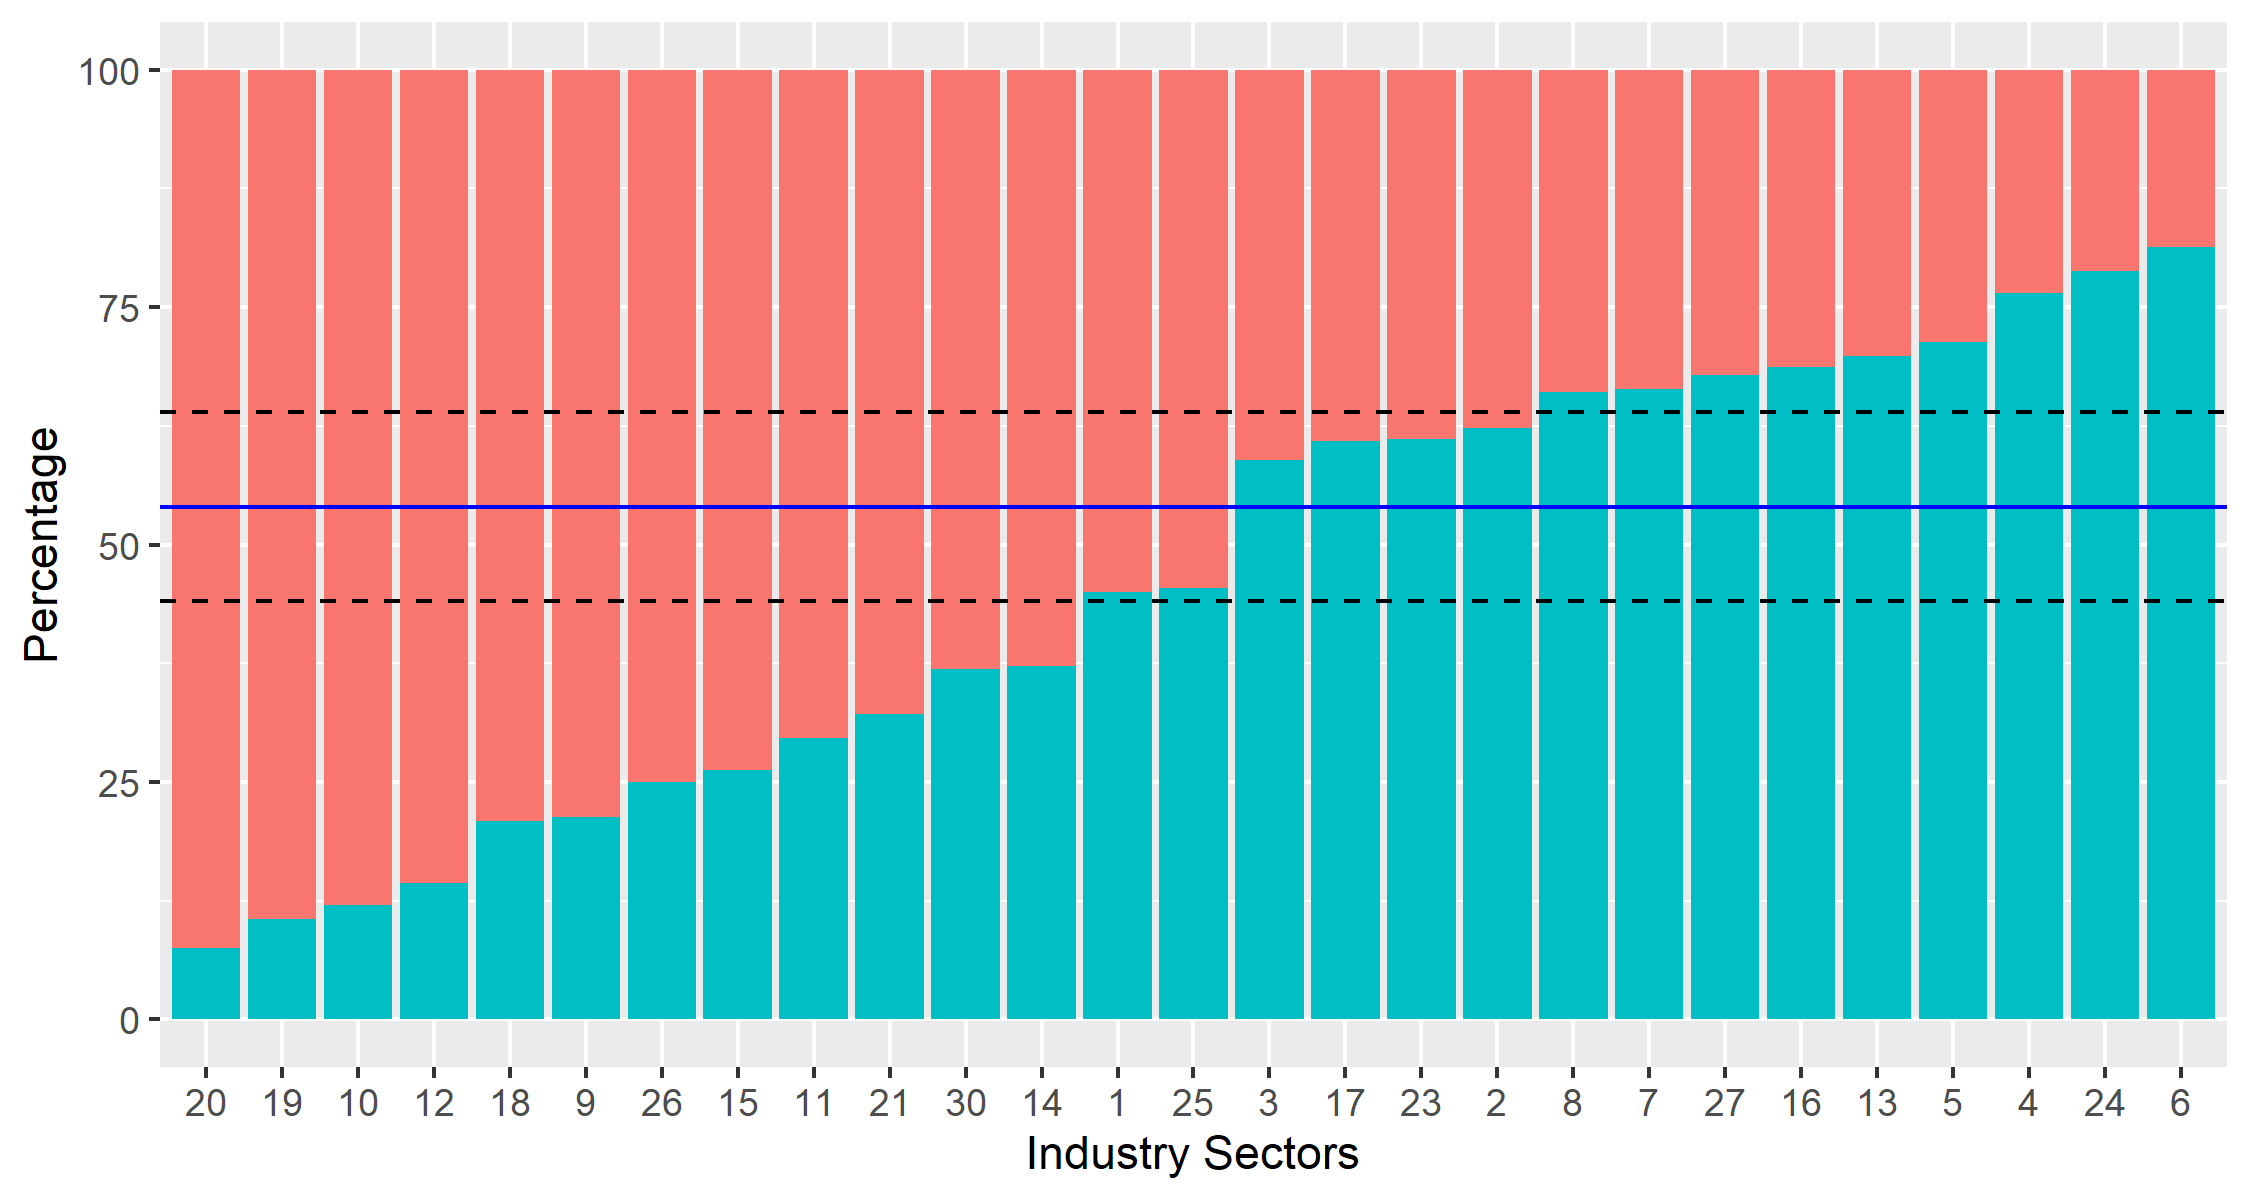
\includegraphics{gen_ind18.png}
	\caption{Distribution of Employment in RLMS 2018 by Industry and Gender}\label{fig:5}
\end{figure}

\begin{figure}[H]
	\centering
	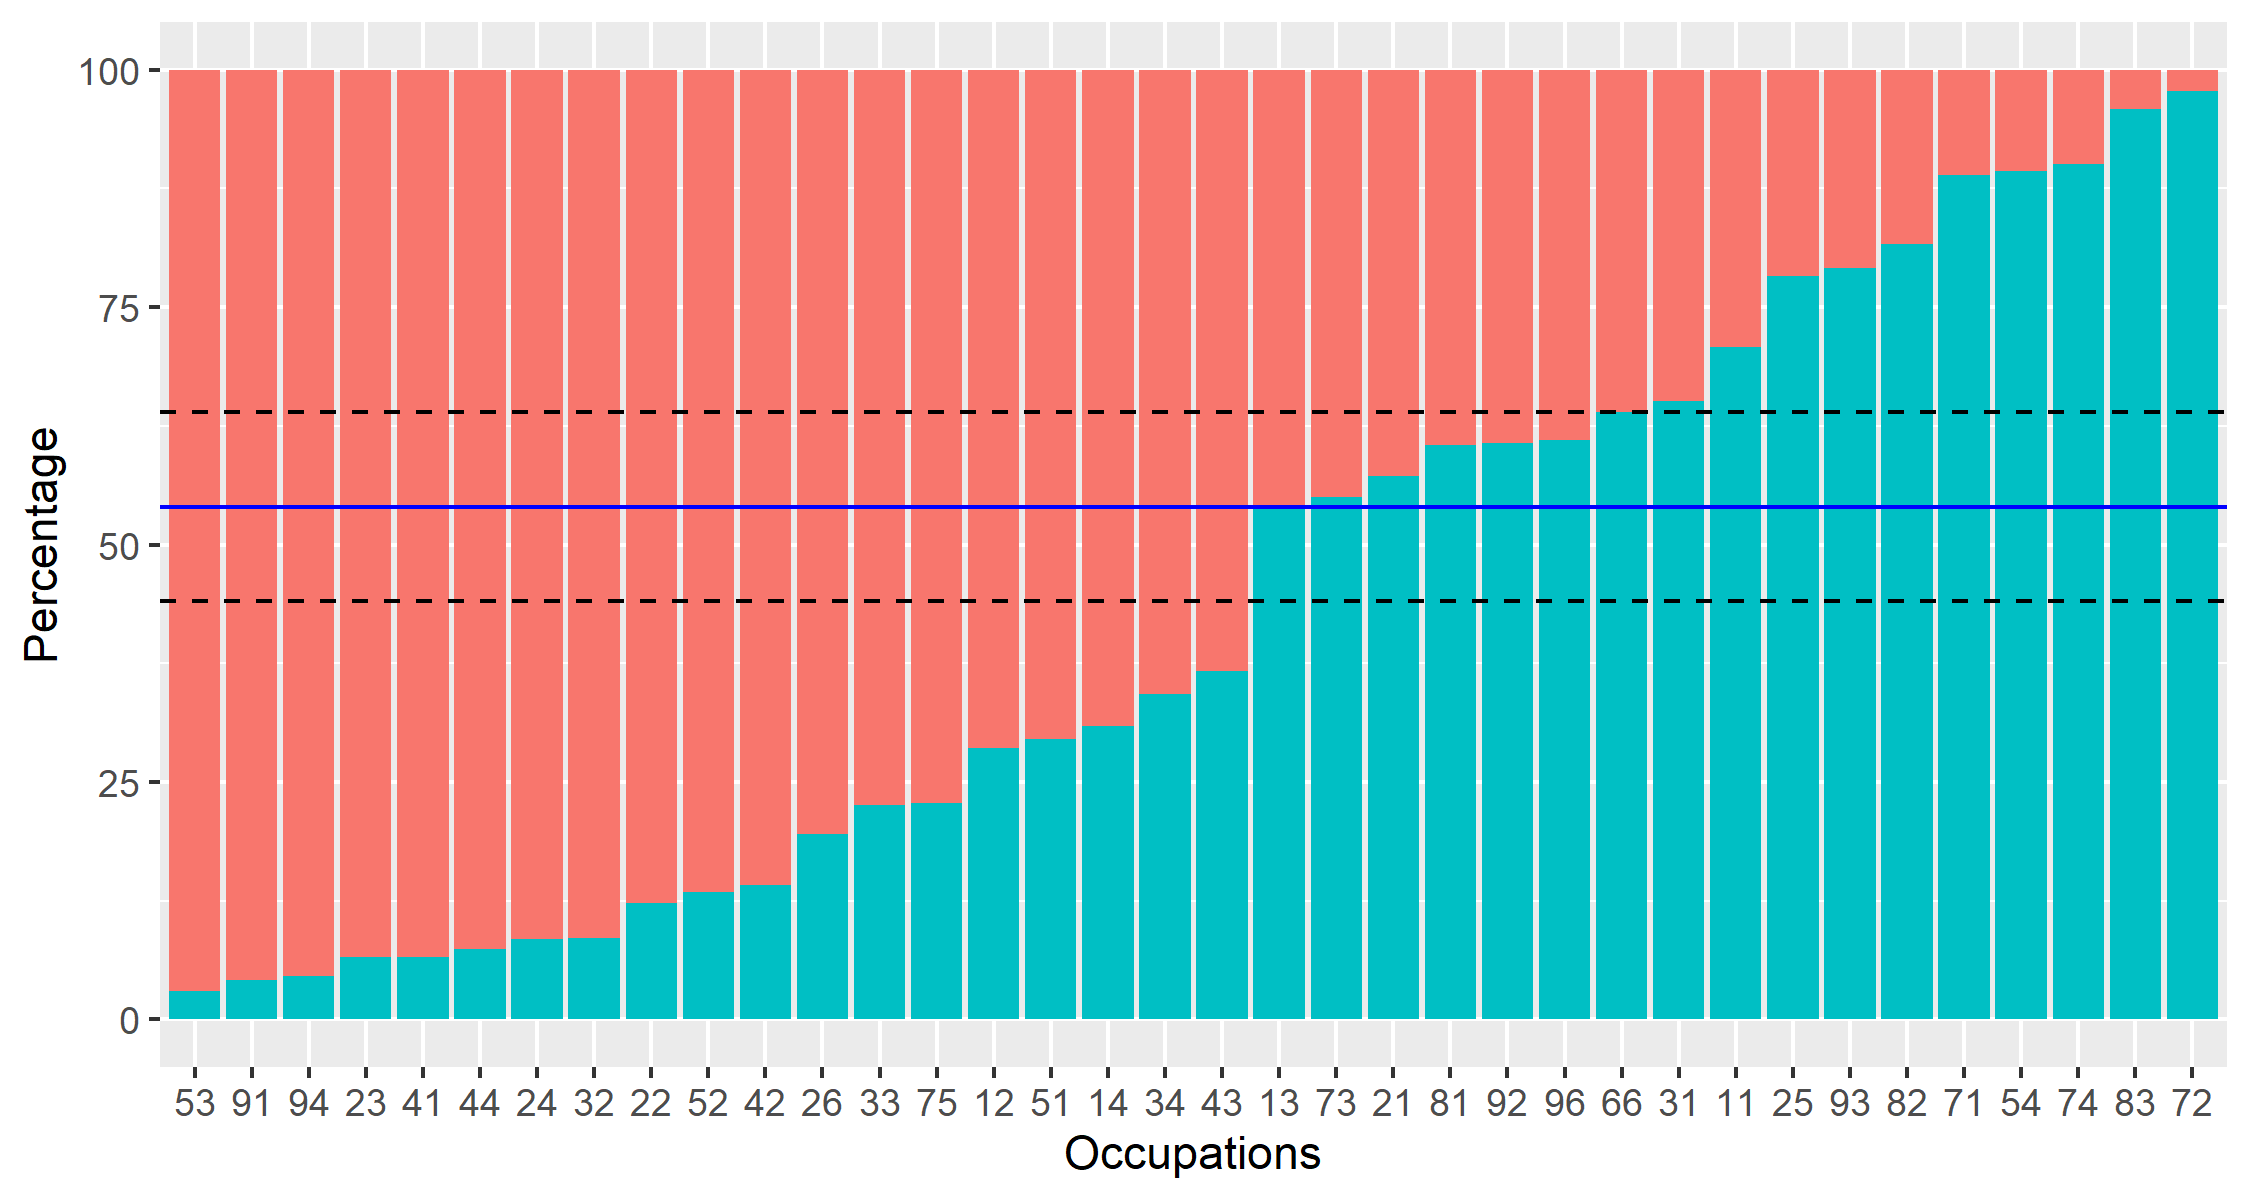
\includegraphics{gen_occ18.png}
	\caption{Distribution of Employment in RLMS 2018 by Industry and Gender}\label{fig:6}
\end{figure}
	
\begin{table}[H]
		\centering
		\def\arraystretch{1} 
		\caption{Industries by Strength of Female Proportion, RLMS 2018}
		\label{tab:4}
		\begin{tabular}{p{2.5cm}l>{\raggedleft\arraybackslash}p{1.5cm}>{\raggedleft\arraybackslash}p{3cm}>{\raggedleft\arraybackslash}p{1.5cm}}
			\hline \hline
			\textbf{Category} & \textbf{Sector} & \textbf{N fem} & \textbf{\% fem} & \textbf{N total} \\ 
			\hline
			Female  & Social Services & 37 & 92.5\% &  40 \\ 
			dominated  & Other & 17 & 89.5\% &  19 \\ 
			& Education & 609 & 88.0\% & 692 \\ 
			& Public Health & 412 & 85.7\% & 481 \\ 
			& Real Estate Operations & 19 & 79.2\% &  24 \\ 
			& Government and Public Administration & 155 & 78.7\% & 197 \\ 
			& General Public Services & 15 & 75.0\% &  20 \\ 
			& Finance & 107 & 73.8\% & 145 \\ 
			& Science, Culture & 100 & 70.4\% & 142 \\ 
			& Jurisprudence & 19 & 67.9\% &  28 \\ \hline
			Neutral & Mass Media, Telecommunications & 24 & 63.2\% &  38 \\ 
			& Trade, Consumer Services & 738 & 62.8\% & 1175 \\ 
			& Light industry, Food industry & 209 & 55.0\% & 380 \\ 
			& Sports, Tourism,Entertainment & 18 & 54.5\% &  33 \\ \hline
			Male & Miltary Industrial Complex & 67 & 41.1\% & 163 \\ 
			dominated & Housing and Community Services & 95 & 39.1\% & 243 \\ 
			& Chemical Industry & 14 & 38.9\% &  36 \\ 
			& Civil Machine Construction & 51 & 37.8\% & 135 \\ 
			& Agriculture & 79 & 33.9\% & 233 \\ 
			& Transportation, Communication & 186 & 33.6\% & 553 \\ 
			& Information Technology & 9 & 32.1\% &  28 \\ 
			& Energy or Power Industry & 41 & 31.3\% & 131 \\ 
			& Army, Internal Security & 90 & 30.1\% & 299 \\ 
			& Other Heavy Industry & 60 & 28.7\% & 209 \\ 
			& Oil and Gas Industry & 52 & 23.5\% & 221 \\ 
			& Wood, Timber, Forestry & 7 & 21.2\% &  33 \\ 
			& Construction & 73 & 18.7\% & 391 \\ \hline
			& Total & 3303 &54.3\% & 6089 \\ \hline
		\end{tabular}
\end{table}
	
\begin{table}[!ht]
	\centering
	\caption{Occupations by Strength of Female Proportion, RLMS 2018}
	\label{tab:5}
		\begin{small}
			\begin{tabular}{cp{10cm}ccc}
				\hline
				& \textbf{Occupation} & \textbf{N fem} & \textbf{\% fem} & \textbf{N total} \\ 
				\hline
				1 & Personal Care Workers & 97 & 97.0\% & 100 \\ 
				2 & Cleaners and Helpers & 163 & 95.9\% & 170 \\ 
				3 & Food Preparation Assistants & 21 & 95.5\% &  22 \\ 
				4 & Teaching Professionals & 370 & 93.4\% & 396 \\ 
				5 & General and Keyboard Clerks & 71 & 93.4\% &  76 \\ 
				6 & Other Clerical Support Workers & 25 & 92.6\% &  27 \\ 
				7 & Business and Administration Professionals & 97 & 91.5\% & 106 \\ 
				8 & Health Associate Professionals & 192 & 91.4\% & 210 \\ 
				9 & Health Professionals & 79 & 87.8\% &  90 \\ 
				10 & Sales Workers & 350 & 86.6\% & 404 \\ 
				11 & Customer Services Clerks & 67 & 85.9\% &  78 \\ 
				12 & Legal, Social and Cultural Professionals & 169 & 80.5\% & 210 \\ 
				13 & Business and Administration Associate Professionals & 517 & 77.4\% & 668 \\ 
				14 & Food Processing, Woodworking, Garment and Other Craft and Related Trades Workers & 51 & 77.3\% &  66 \\ 
				15 & Administrative and Commercial Managers & 25 & 71.4\% &  35 \\ 
				16 & Personal Services Workers & 172 & 70.5\% & 244 \\ 
				17 & Hospitality, Retail and Other Services Managers & 38 & 69.1\% &  55 \\ 
				18 & Legal, Social, Cultural and Related Associate Professionals & 69 & 65.7\% & 105 \\ \hline
				19 & Numerical and Material Recording Clerks & 100 & 63.3\% & 158 \\ 
				20 & Production and Specialized Services Managers & 139 & 46.0\% & 302 \\ 
				21 & Handicraft and Printing Workers & 9 & 45.0\% &  20 \\ \hline
				22 & Science and Engineering Professionals & 101 & 42.8\% & 236 \\ 
				23 & Stationary Plant and Machine Operators & 72 & 39.6\% & 182 \\ 
				24 & Agricultural, Forestry and Fishery Labourers & 11 & 39.3\% &  28 \\ 
				25 & Refuse Workers and Other Elementary Workers & 30 & 39.0\% &  77 \\ 
				26 & Miscellaneous non-ISCO & 9 & 36.0\% &  25 \\ 
				27 & Science and Engineering Associate Professionals & 120 & 34.9\% & 344 \\ 
				28 & Chief Executives, Senior Officials and Legislators & 7 & 29.2\% &  24 \\ 
				29 & Information and Communications Technology Professionals & 15 & 21.7\% &  69 \\ 
				30 & Labourers in Mining, Construction, Manufacturing and Transport & 24 & 20.9\% & 115 \\ 
				31 & Assemblers & 11 & 18.3\% &  60 \\ 
				32 & Building and Related Trades Workers (excluding Electricians) & 23 & 11.1\% & 207 \\ 
				33 & Protective Services Workers & 23 & 10.7\% & 215 \\ 
				34 & Electrical and Electronic Trades Workers & 16 & 9.9\% & 162 \\ 
				35 & Drivers and Mobile Plant Operators & 23 & 4.1\% & 558 \\ 
				36 & Metal, Machinery and Related Trades Workers & 6 & 2.2\% & 267 \\ 
				\hline
			\end{tabular}
		\end{small}
	\end{table}

Table \ref{tab:6} depicts average rates of human capital loss due to experience and education by the female- and male-dominated industrial sectors and occupations. It can be seen that the human capital depreciation rate due to experience for industries in which females outweigh is equal to 0.89\%, whereas for the ones where males prevail is equal to 1.82\%. However, these numbers are not different statistically (even 90\% confidence bands cross each other). A similar pattern was registered concerning experience depreciation for female- and male-dominated occupations: the estimated parameters are not distinguishable for the general population. 

As for education obsolescence rates, in all the groups under focus, this measure is nil at any conventional level of significance.

\begin{table}[H]
	\centering 
	\caption{Average Human Capital Depreciation Rates (DR) by Female- and Male-dominated Industries and Occupations, RLMS 2018} 
	\label{tab:6} 
	\begin{tabular}{clcccc}
		\hline
		& \textbf{Statistic} &\textbf{Ind\_F}& \textbf{Ind\_M} & \textbf{occfemale} & \textbf{occmale} \\ 
		\hline
		1 & Experience, mean & 14.06 & 13.01 & 13.67 & 12.67 \\ 
		2 & Education, mean & 23.45 & 22.97 & 21.67 & 23.48 \\ 
		\midrule
		3 & DR Experience, \% & 0.89 & 1.82 & 1.55 & 1.40 \\ 
		4 & DR Education, \% & 0.00 & 0.00 & 0.00 & 0.00 \\ 
		5 & DR Human Capital, \% & 0.89 & 1.82 & 1.55 & 1.40 \\ 
		\hline
	\end{tabular}
\end{table} 


\subsection{Depreciation and Occupational Routineness}

In addition to the examination of human capital depreciation rates in gender-dominated industries and occupations, we explored this parameter between groups generated by using an array of routine and non-routine task content metrics for ISCO-08. In this analysis, we rely on measures developed by \citet{mihaylov_152._2019}. Particularity, Routine Task Intensity measure (RTI) -- a variable of interest -- denoted a score difference between the summed routine task indices and the summed non-routine task indices: $(RC + RM) - (NRA + NRI + NRM)$. Besides, we introduced a separate measure by bringing together the non-routine task indices: $NRA + NRI + NRM$. Further, exploiting the k-means clustering technique, for the metrics described, we created two respective categorical variables (drti and dnraim) with categories capturing \textit{high, medium,} and \textit{low} manifestations of the features.

Table \ref{tab:7} shows the results of comparing depreciation rates between individuals whose jobs invoke routine or non-routine tasks at a high, medium, or low level. The findings suggest that depreciation explained by experience does not differ substantially between people with various routine task intensity (due to confidence limits crossing, not shown). The same outcome also applies to workers varying in the degree of non-routine content at their jobs. Human capital loss due to education is equal to zero for each of the groups analyzed.

\begin{table}[H]
	\centering
	\caption{Average Human Capital Depreciation Rates (DR) by Routineness Classification, RLMS 2018}
	\label{tab:7}
	\begin{tabular}{clccccccccc}
		\hline
		& \textbf{Statistic} & \textbf{High} & \textbf{Low} & \textbf{Medium} & \textbf{High} & \textbf{Low} & \textbf{Medium} \\ 
		\hline
		1 & Measure & drti & drti & drti & dnraim & dnraim & dnraim \\ 
		2 & Experience, mean & 12.86 & 13.67 & 12.8 & 13.66 & 12.76 & 13.02 \\ 
		3 & Education, mean & 21.44 & 22.79 & 22.76 & 22.94 & 22.22 & 22.05 \\ 
		\midrule
		4 & DR Experience, \% & 1.8 & 1.5 & 1.64 & 1.62 & 1.73 & 1.48 \\ 
		5 & DR Education, \% & 0 & 0 & 0 & 0 & 0 & 0 \\ 
		6 & DR Human Capital, \% & 1.8 & 1.5 & 1.64 & 1.62 & 1.73 & 1.48 \\ 
		\hline
	\end{tabular}
\end{table}

\section{The Analysis of Regional Returns to Education \\ in the Russian Federation}

\subsection{Data}
To estimate returns to education in Russian regions, we used a Statistical Survey of Income and Participation in Social Programs, collected by Rosstat. The primary purpose of the Rosstat survey was to obtain statistical information, reflecting the role of wages, income from self-employment, property income, pensions, and social benefits in ensuring the material well-being of families. The survey contains data on trends in income and poverty variation among households with different socio-economic status. There are also variables on people's participation in social programs, their pension and health insurance, material and social security of low-income families, and the impact of social policy measures on people's well-being.

The 2018 data (the most recent year of the survey) was exploited in the current section. A sub-sample selected for the empirical modeling is identical to the one used for the RLMS analysis: individuals aged 25-64 who are out of school and have positive labor market experience and income.

\subsection{Methods}

The classical Mincerian equation (described in the previous sections) was the main focus in the regional investigation of returns to education in Russia: we looked at how these returns vary across regions. Additionally, we took a step further and explored the determinants of the established variation. For this purpose, a multilevel regression analysis (mixed modeling) was leveraged. The equations of interest are as follows:

\textbf{First level:}
$$Log(Wage)_{ij} = b_{0j} + b_{1j}\cdot Educ + b_{2j}\cdot Exp + b_{3j}\cdot Exp^2 + b_{4j}\cdot Gender + \epsilon_{ij}$$

\textbf{Second Level:}
$$b_{0j} = \gamma_{00} + \gamma_{0n}\cdot Z + u_{00}$$
$$b_{1j} = \gamma_{10} + \gamma_{1n}\cdot Z + u_{10} $$
$$b_{ij} = \gamma_{i0} \quad for \quad i \neq 0$$

\noindent
where an individual $i$ is nested withing a region $j$, $Log(Wage)$ is a logarithm of monthly wage, $Educ$ stands for highest attained level of education, $Exp$ and $Exp^2$ reflect the years of working experience and its quadratic term respectively, $Gender$ is a dummy variable for gender, $Z$ is an $n\times i$ matrix of regional characteristics, $\epsilon$ and $u_{00}$, $u_{10}$ are the first- and second-level errors respectively.
\\

Mixed models were estimated using restricted maximum likelihood (REML). Individual Wald tests and likelihood ratio tests were exploited to evaluate the significance of fixed and random effects, respectively. It should be noted that we also used weights in the modeling to ensure the representativeness of the sample across Russian regions (the weighting variable was divided by 1000 to allow the convergence of the multilevel models). 

\subsection{Measures}

\subsubsection{Dependent variable}
Similar to the previous analyses, a logged amount of money remuneration before income tax payment at the main place of work (R\_DEN) was utilized as an outcome of interest.

\subsubsection{Independent variables}
Education, working experience, and gender were treated as the first-level independent variables. Education (I01\_10) -- a central predictor --- was plugged into the multilevel models in its categorical form. Gender (H01\_01) was leveraged as a dichotomous variable. To calculate the labor market experience variable, we relied on the same naive strategy as in the previous section.

The predictors used at the second level were as follows: \textit{gross regional product, urbanization level, coverage by higher and vocational education (the number of students per 10,000 people in a region), quality of education, regional unemployment level} and \textit{a share of people in jobs related to natural resources}. Quality of education measure reflected a regional performance of students on the EGE - a Russian school-leaving exam (see Parandekar and Shmis 2018 for the details of the variable generation). The rest of the attributes were taken from the Rosstat website. Table \ref{tab:8} demonstrates a descriptive statistics by regions.

\fontsize{9}{11}{
	\selectfont
	\setlength{\tabcolsep}{3pt}
	\begin{longtable}{lcccccccccc}
		\caption{Descriptive Statistics for the Variables by Regions in Russia, Rosstat 2018}
		\label{tab:8}\\
	    \hline
		&  & \multicolumn{2}{c}{\textbf{Wage}} & \multicolumn{2}{c}{\textbf{Experience}} & \multicolumn{3}{c}{\textbf{Education, \%}} & \multicolumn{2}{c}{\textbf{Gender, \%}} \\ 
		\textbf{Regions}  & \textbf{N} & \textbf{mean} & \textbf{sd} & \textbf{mean} & \textbf{sd} & \textbf{SE} & \textbf{VE} & \textbf{HE} & \textbf{Males} & \multicolumn{1}{c}{\textbf{Females}} \\ 
		\hline
		\endhead
		Altayskiy Kray  & $\phantom{0}4646$ & $22127.6$ & $11952.2$ & $\phantom{000}23.6$ & $\phantom{000}11.0$ & $17.456$ & $54.50$ & $28.05$ & $48.90$ & $51.10$ \\
		Amurskaya Oblast  & $\phantom{0}2557$ & $33441.2$ & $17409.0$ & $\phantom{000}23.2$ & $\phantom{000}11.2$ & $16.347$ & $50.65$ & $33.01$ & $49.59$ & $50.41$ \\
		Arkhangelskaya Oblast  & $\phantom{0}3183$ & $33438.1$ & $16884.2$ & $\phantom{000}22.6$ & $\phantom{000}10.6$ & $12.692$ & $54.95$ & $32.36$ & $44.17$ & $55.83$ \\
		Astrakhanskaya Oblast  & $\phantom{0}2836$ & $26474.1$ & $13737.6$ & $\phantom{000}23.0$ & $\phantom{000}11.3$ & $13.646$ & $55.08$ & $31.28$ & $50.99$ & $49.01$ \\
		Belgorodskaya Oblast  & $\phantom{0}3692$ & $26281.0$ & $10811.9$ & $\phantom{000}23.8$ & $\phantom{000}11.1$ & $12.351$ & $54.47$ & $33.18$ & $49.76$ & $50.24$ \\
		Bryanskaya Oblast  & $\phantom{0}3087$ & $22482.3$ & $\phantom{0}9634.1$ & $\phantom{000}23.5$ & $\phantom{000}10.9$ & $19.631$ & $50.66$ & $29.71$ & $48.66$ & $51.34$ \\
		Chechenskaya Respublika  & $\phantom{0}2010$ & $27718.4$ & $11793.2$ & $\phantom{000}18.7$ & $\phantom{000}10.6$ & $25.721$ & $26.37$ & $47.91$ & $65.37$ & $34.63$ \\
		Chelyabinskaya Oblast  & $\phantom{0}6717$ & $27990.8$ & $14280.9$ & $\phantom{000}23.9$ & $\phantom{000}11.2$ & $12.104$ & $54.53$ & $33.36$ & $47.39$ & $52.61$ \\
		Chukotskiy Aok  & $\phantom{0}1535$ & $65574.1$ & $32370.8$ & $\phantom{000}23.6$ & $\phantom{000}10.6$ & $13.941$ & $46.06$ & $40.00$ & $43.97$ & $56.03$ \\
		Chuvashskaya Respublika  & $\phantom{0}3248$ & $21453.7$ & $12602.2$ & $\phantom{000}24.3$ & $\phantom{000}11.0$ & $19.119$ & $50.80$ & $30.08$ & $50.18$ & $49.82$ \\
		Evreyskaya AOb  & $\phantom{0}1536$ & $28532.1$ & $17385.1$ & $\phantom{000}23.8$ & $\phantom{000}11.2$ & $22.005$ & $50.33$ & $27.67$ & $50.00$ & $50.00$ \\
		Irkutskaya Oblast  & $\phantom{0}4686$ & $29967.6$ & $17443.1$ & $\phantom{000}22.3$ & $\phantom{000}11.2$ & $17.520$ & $47.06$ & $35.42$ & $47.57$ & $52.43$ \\
		Ivanovskaya Oblast  & $\phantom{0}2876$ & $24881.8$ & $12496.8$ & $\phantom{000}23.3$ & $\phantom{000}10.9$ & $20.341$ & $49.90$ & $29.76$ & $47.77$ & $52.23$ \\
		Kabardino-Balkarskaya Res.  & $\phantom{0}2006$ & $23592.3$ & $10766.2$ & $\phantom{000}21.7$ & $\phantom{000}11.6$ & $21.137$ & $40.53$ & $38.33$ & $52.04$ & $47.96$ \\
		Kaliningradskaya Oblast  & $\phantom{0}2838$ & $29749.2$ & $15489.1$ & $\phantom{000}23.5$ & $\phantom{000}11.4$ & $13.495$ & $52.40$ & $34.11$ & $50.07$ & $49.93$ \\
		Kaluzhskaya Oblast  & $\phantom{0}3155$ & $29662.1$ & $12879.5$ & $\phantom{000}24.1$ & $\phantom{000}11.2$ & $13.312$ & $52.11$ & $34.58$ & $47.92$ & $52.08$ \\
		Kamchatskaya Kray  & $\phantom{0}2203$ & $51160.5$ & $29997.7$ & $\phantom{000}23.1$ & $\phantom{000}11.2$ & $13.118$ & $42.99$ & $43.89$ & $47.89$ & $52.11$ \\
		Karachayevo-Cherkessiya  & $\phantom{0}1510$ & $22900.6$ & $12540.8$ & $\phantom{000}22.0$ & $\phantom{000}11.8$ & $17.152$ & $40.07$ & $42.78$ & $48.01$ & $51.99$ \\
		Kemerovskaya Oblast  & $\phantom{0}5056$ & $26287.0$ & $13774.4$ & $\phantom{000}23.6$ & $\phantom{000}11.3$ & $18.137$ & $52.99$ & $28.88$ & $48.04$ & $51.96$ \\
		Khabarovskiy Kray  & $\phantom{0}3731$ & $42008.8$ & $21837.8$ & $\phantom{000}22.3$ & $\phantom{000}11.2$ & $11.900$ & $44.33$ & $43.77$ & $46.15$ & $53.85$ \\
		Khanty-Mansiyskiy Aok  & $\phantom{0}4335$ & $50837.9$ & $22261.7$ & $\phantom{000}22.8$ & $\phantom{000}10.5$ & $13.564$ & $46.78$ & $39.65$ & $49.60$ & $50.40$ \\
		Kirovskaya Oblast  & $\phantom{0}3284$ & $22941.0$ & $13674.6$ & $\phantom{000}25.1$ & $\phantom{000}11.2$ & $20.128$ & $55.33$ & $24.54$ & $47.69$ & $52.31$ \\
		Kostromskaya Oblast  & $\phantom{0}2518$ & $23993.1$ & $12090.9$ & $\phantom{000}23.6$ & $\phantom{000}11.1$ & $12.669$ & $61.28$ & $26.05$ & $47.82$ & $52.18$ \\
		Krasnodarskiy Kray  & $\phantom{0}8730$ & $32563.7$ & $17499.8$ & $\phantom{000}23.0$ & $\phantom{000}10.9$ & $15.888$ & $48.57$ & $35.54$ & $50.02$ & $49.98$ \\
		Krasnoyarskiy Kray  & $\phantom{0}5540$ & $33954.6$ & $21199.2$ & $\phantom{000}23.0$ & $\phantom{000}11.0$ & $21.588$ & $48.05$ & $30.36$ & $49.64$ & $50.36$ \\
		Kurganskaya Oblast  & $\phantom{0}2468$ & $20896.9$ & $11539.5$ & $\phantom{000}24.4$ & $\phantom{000}10.7$ & $21.394$ & $52.47$ & $26.13$ & $48.38$ & $51.62$ \\
		Kurskaya Oblast  & $\phantom{0}2956$ & $23622.6$ & $11475.0$ & $\phantom{000}23.9$ & $\phantom{000}11.0$ & $14.783$ & $52.17$ & $33.05$ & $50.30$ & $49.70$ \\
		Leningradskaya Oblast  & $\phantom{0}4506$ & $32124.3$ & $17227.4$ & $\phantom{000}24.2$ & $\phantom{000}11.5$ & $\phantom{0}7.723$ & $54.77$ & $37.51$ & $46.03$ & $53.97$ \\
		Lipetskaya Oblast  & $\phantom{0}2869$ & $25037.8$ & $10813.5$ & $\phantom{000}24.1$ & $\phantom{000}11.0$ & $13.106$ & $53.82$ & $33.08$ & $49.60$ & $50.40$ \\
		Magadanskaya Oblast  & $\phantom{0}1841$ & $51000.8$ & $23729.4$ & $\phantom{000}24.1$ & $\phantom{000}11.4$ & $18.523$ & $43.02$ & $38.46$ & $43.24$ & $56.76$ \\
		Moscow  & $29921$ & $66263.5$ & $26437.9$ & $\phantom{000}20.8$ & $\phantom{000}10.8$ & $\phantom{0}4.953$ & $32.18$ & $62.86$ & $47.06$ & $52.94$ \\
		Moskovskaya Oblast  & $13431$ & $46725.1$ & $20563.7$ & $\phantom{000}22.6$ & $\phantom{000}11.4$ & $10.975$ & $39.13$ & $49.89$ & $47.51$ & $52.49$ \\
		Murmanskaya Oblast  & $\phantom{0}3078$ & $43992.5$ & $28841.9$ & $\phantom{000}23.4$ & $\phantom{000}11.2$ & $12.801$ & $50.45$ & $36.74$ & $49.84$ & $50.16$ \\
		Nenetskiy Aok  & $\phantom{0}1118$ & $54467.3$ & $23147.1$ & $\phantom{000}22.6$ & $\phantom{000}10.8$ & $17.263$ & $49.73$ & $33.01$ & $39.98$ & $60.02$ \\
		Nizhegorodskaya Oblast  & $\phantom{0}6139$ & $30912.9$ & $13291.8$ & $\phantom{000}23.4$ & $\phantom{000}11.2$ & $16.941$ & $49.31$ & $33.75$ & $47.42$ & $52.58$ \\
		Novgorodskaya Oblast  & $\phantom{0}2673$ & $26856.0$ & $12683.0$ & $\phantom{000}24.6$ & $\phantom{000}11.2$ & $15.638$ & $55.74$ & $28.62$ & $45.16$ & $54.84$ \\
		Novosibirskaya Oblast  & $\phantom{0}5374$ & $29229.9$ & $14687.7$ & $\phantom{000}23.9$ & $\phantom{000}11.6$ & $16.561$ & $49.33$ & $34.11$ & $47.06$ & $52.94$ \\
		Omskaya Oblast  & $\phantom{0}3978$ & $25337.5$ & $14613.1$ & $\phantom{000}23.6$ & $\phantom{000}10.9$ & $22.197$ & $51.31$ & $26.50$ & $51.11$ & $48.89$ \\
		Orenburgskaya Oblast  & $\phantom{0}4190$ & $24207.0$ & $12519.9$ & $\phantom{000}23.3$ & $\phantom{000}11.0$ & $15.131$ & $53.68$ & $31.19$ & $51.29$ & $48.71$ \\
		Orlovskaya Oblast  & $\phantom{0}2424$ & $21901.2$ & $10561.0$ & $\phantom{000}24.7$ & $\phantom{000}11.1$ & $15.017$ & $50.66$ & $34.32$ & $46.99$ & $53.01$ \\
		Penzenskaya Oblast  & $\phantom{0}3103$ & $23478.4$ & $10982.9$ & $\phantom{000}24.2$ & $\phantom{000}11.0$ & $20.722$ & $51.40$ & $27.88$ & $51.02$ & $48.98$ \\
		Permskiy Krai  & $\phantom{0}5290$ & $29176.6$ & $14449.4$ & $\phantom{000}23.4$ & $\phantom{000}11.0$ & $13.894$ & $58.32$ & $27.79$ & $48.17$ & $51.83$ \\
		Primorskiy Kray  & $\phantom{0}4104$ & $37839.9$ & $18420.2$ & $\phantom{000}23.8$ & $\phantom{000}11.3$ & $14.985$ & $52.97$ & $32.04$ & $49.98$ & $50.02$ \\
		Pskovskaya Oblast  & $\phantom{0}2382$ & $23838.4$ & $12015.3$ & $\phantom{000}25.0$ & $\phantom{000}11.0$ & $17.632$ & $55.33$ & $27.04$ & $48.11$ & $51.89$ \\
		Respublika Adygeya  & $\phantom{0}2013$ & $21350.3$ & $10505.9$ & $\phantom{000}23.4$ & $\phantom{000}11.3$ & $20.666$ & $43.67$ & $35.67$ & $49.53$ & $50.47$ \\
		Respublika Altay  & $\phantom{0}1381$ & $20285.3$ & $12029.5$ & $\phantom{000}23.0$ & $\phantom{000}10.6$ & $23.027$ & $45.26$ & $31.72$ & $43.08$ & $56.92$ \\
		Respublika Bashkortostan  & $\phantom{0}7126$ & $31100.8$ & $15175.2$ & $\phantom{000}23.4$ & $\phantom{000}11.0$ & $12.167$ & $56.67$ & $31.17$ & $51.98$ & $48.02$ \\
		Respublika Buryatia  & $\phantom{0}2469$ & $29536.3$ & $17237.4$ & $\phantom{000}22.1$ & $\phantom{000}10.6$ & $17.173$ & $45.61$ & $37.22$ & $48.12$ & $51.88$ \\
		Respublika Crimea  & $\phantom{0}2895$ & $19916.2$ & $\phantom{0}9743.9$ & $\phantom{000}22.8$ & $\phantom{000}11.0$ & $21.244$ & $43.90$ & $34.85$ & $52.99$ & $47.01$ \\
		Respublika Dagestan  & $\phantom{0}3388$ & $26377.3$ & $11971.9$ & $\phantom{000}23.0$ & $\phantom{000}10.7$ & $30.519$ & $30.79$ & $38.70$ & $55.99$ & $44.01$ \\
		Respublika Ingushetiya  & $\phantom{0}1207$ & $23740.2$ & $10168.5$ & $\phantom{000}18.2$ & $\phantom{0000}9.6$ & $10.025$ & $18.89$ & $71.09$ & $61.14$ & $38.86$ \\
		Respublika Kalmykiya  & $\phantom{0}1751$ & $18568.8$ & $11749.1$ & $\phantom{000}23.6$ & $\phantom{000}11.4$ & $15.762$ & $40.89$ & $43.35$ & $46.43$ & $53.57$ \\
		Respublika Karelia  & $\phantom{0}2164$ & $28510.2$ & $16639.5$ & $\phantom{000}23.7$ & $\phantom{000}10.8$ & $17.144$ & $55.45$ & $27.40$ & $47.00$ & $53.00$ \\
		Respublika Khakasiya  & $\phantom{0}2064$ & $27288.1$ & $16613.3$ & $\phantom{000}23.3$ & $\phantom{000}11.1$ & $22.045$ & $51.11$ & $26.84$ & $50.97$ & $49.03$ \\
		Respublika Komi  & $\phantom{0}2972$ & $35891.6$ & $21554.4$ & $\phantom{000}23.8$ & $\phantom{000}11.0$ & $16.689$ & $53.47$ & $29.85$ & $46.67$ & $53.33$ \\
		Respublika Mariy El  & $\phantom{0}2486$ & $21133.1$ & $11941.6$ & $\phantom{000}24.1$ & $\phantom{000}11.2$ & $18.785$ & $52.98$ & $28.24$ & $47.87$ & $52.13$ \\
		Respublika Mordovia  & $\phantom{0}2236$ & $21221.0$ & $10837.3$ & $\phantom{000}23.1$ & $\phantom{000}11.2$ & $15.519$ & $49.11$ & $35.38$ & $48.35$ & $51.65$ \\
		Respublika Saha (Yakutia)  & $\phantom{0}3243$ & $45763.1$ & $25001.6$ & $\phantom{000}23.2$ & $\phantom{000}11.3$ & $18.440$ & $45.76$ & $35.80$ & $46.69$ & $53.31$ \\
		Respublika Severnaya Osetiya  & $\phantom{0}2114$ & $22993.1$ & $12762.5$ & $\phantom{000}21.8$ & $\phantom{000}11.3$ & $12.677$ & $40.92$ & $46.40$ & $48.91$ & $51.09$ \\
		Respublika Tatarstan  & $\phantom{0}7212$ & $30327.9$ & $12928.8$ & $\phantom{000}23.5$ & $\phantom{000}11.1$ & $18.691$ & $48.64$ & $32.67$ & $51.48$ & $48.52$ \\
		Respublika Tyva  & $\phantom{0}1704$ & $23421.9$ & $16851.3$ & $\phantom{000}21.4$ & $\phantom{000}10.0$ & $19.777$ & $44.78$ & $35.45$ & $40.43$ & $59.57$ \\
		Rostovskaya Oblast  & $\phantom{0}6985$ & $28287.2$ & $12779.9$ & $\phantom{000}23.1$ & $\phantom{000}11.0$ & $15.476$ & $48.03$ & $36.49$ & $50.68$ & $49.32$ \\
		Ryazanskaya Oblast  & $\phantom{0}2609$ & $25889.2$ & $11760.9$ & $\phantom{000}24.7$ & $\phantom{000}11.1$ & $12.457$ & $59.37$ & $28.17$ & $49.18$ & $50.82$ \\
		Saint-Petersburg  & $11352$ & $48520.8$ & $23771.0$ & $\phantom{000}22.8$ & $\phantom{000}11.4$ & $\phantom{0}5.259$ & $38.15$ & $56.59$ & $46.04$ & $53.96$ \\
		Sakhalinskaya Oblast  & $\phantom{0}2258$ & $50325.1$ & $25563.0$ & $\phantom{000}23.6$ & $\phantom{000}11.2$ & $17.493$ & $48.23$ & $34.28$ & $46.94$ & $53.06$ \\
		Samarskaya Oblast  & $\phantom{0}6275$ & $32584.4$ & $15015.6$ & $\phantom{000}23.8$ & $\phantom{000}11.1$ & $11.331$ & $47.87$ & $40.80$ & $47.71$ & $52.29$ \\
		Saratovskaya Oblast  & $\phantom{0}4572$ & $23698.6$ & $12322.4$ & $\phantom{000}23.7$ & $\phantom{000}10.8$ & $14.961$ & $50.22$ & $34.82$ & $50.42$ & $49.58$ \\
		Sevastopol  & $\phantom{0}1489$ & $24811.3$ & $13498.9$ & $\phantom{000}22.4$ & $\phantom{000}11.2$ & $\phantom{0}9.671$ & $44.93$ & $45.40$ & $53.32$ & $46.68$ \\
		Smolenskaya Oblast  & $\phantom{0}2726$ & $25517.8$ & $12104.9$ & $\phantom{000}24.6$ & $\phantom{000}11.3$ & $14.380$ & $52.31$ & $33.31$ & $46.04$ & $53.96$ \\
		Stavropolskiy Kray  & $\phantom{0}4945$ & $25263.6$ & $12696.7$ & $\phantom{000}22.6$ & $\phantom{000}11.3$ & $16.946$ & $43.80$ & $39.25$ & $47.48$ & $52.52$ \\
		Sverdlovskaya Oblast  & $\phantom{0}7712$ & $35983.2$ & $15242.7$ & $\phantom{000}23.6$ & $\phantom{000}11.3$ & $16.779$ & $54.94$ & $28.28$ & $48.59$ & $51.41$ \\
		Tambovskaya Oblast  & $\phantom{0}2781$ & $22698.6$ & $10440.1$ & $\phantom{000}24.1$ & $\phantom{000}11.0$ & $16.397$ & $53.54$ & $30.06$ & $50.67$ & $49.33$ \\
		Tomskaya Oblast  & $\phantom{0}3074$ & $29580.6$ & $16745.7$ & $\phantom{000}22.1$ & $\phantom{000}11.1$ & $13.500$ & $47.56$ & $38.94$ & $46.78$ & $53.22$ \\
		Tulskaya Oblast  & $\phantom{0}3516$ & $27687.4$ & $11814.7$ & $\phantom{000}24.3$ & $\phantom{000}11.3$ & $17.491$ & $54.69$ & $27.82$ & $48.98$ & $51.02$ \\
		Tverskaya Oblast  & $\phantom{0}3157$ & $26310.0$ & $15025.1$ & $\phantom{000}25.5$ & $\phantom{000}11.1$ & $14.824$ & $56.57$ & $28.60$ & $44.73$ & $55.27$ \\
		Tyumenskaya Oblast  & $\phantom{0}3095$ & $31441.2$ & $17278.6$ & $\phantom{000}22.7$ & $\phantom{000}11.2$ & $16.123$ & $52.89$ & $30.99$ & $50.05$ & $49.95$ \\
		Udmurtskaya Respublika  & $\phantom{0}4073$ & $24044.6$ & $11540.9$ & $\phantom{000}23.9$ & $\phantom{000}11.3$ & $20.108$ & $51.04$ & $28.85$ & $46.99$ & $53.01$ \\
		Ul'yanovskaya Oblast  & $\phantom{0}3109$ & $23215.3$ & $10596.4$ & $\phantom{000}24.8$ & $\phantom{000}10.9$ & $19.170$ & $53.84$ & $26.99$ & $50.37$ & $49.63$ \\
		Vladimirskaya Oblast  & $\phantom{0}3502$ & $25001.4$ & $12605.8$ & $\phantom{000}24.5$ & $\phantom{000}11.4$ & $19.503$ & $50.77$ & $29.73$ & $46.49$ & $53.51$ \\
		Volgogradskaya Oblast  & $\phantom{0}4836$ & $24459.0$ & $12915.8$ & $\phantom{000}23.2$ & $\phantom{000}11.0$ & $15.881$ & $50.91$ & $33.21$ & $49.69$ & $50.31$ \\
		Vologodskaya Oblast  & $\phantom{0}2965$ & $28248.9$ & $16693.8$ & $\phantom{000}23.9$ & $\phantom{000}11.2$ & $17.302$ & $57.47$ & $25.23$ & $49.61$ & $50.39$ \\
		Voronezhskaya Oblast  & $\phantom{0}4348$ & $26261.9$ & $11813.9$ & $\phantom{000}23.6$ & $\phantom{000}11.5$ & $22.700$ & $43.38$ & $33.92$ & $48.37$ & $51.63$ \\
		Yamalo-Nenetskiy Aok  & $\phantom{0}3164$ & $69356.7$ & $28075.6$ & $\phantom{000}21.0$ & $\phantom{000}10.4$ & $10.683$ & $40.27$ & $49.05$ & $48.74$ & $51.26$ \\
		Yaroslavskaya Oblast  & $\phantom{0}3361$ & $30261.4$ & $14682.8$ & $\phantom{000}24.1$ & $\phantom{000}11.4$ & $16.215$ & $53.73$ & $30.05$ & $47.01$ & $52.99$ \\
		Zabaykalskiy Kray  & $\phantom{0}3017$ & $28336.6$ & $16350.4$ & $\phantom{000}23.0$ & $\phantom{000}10.6$ & $24.561$ & $47.40$ & $28.04$ & $47.07$ & $52.93$ \\
		\hline 
	\end{longtable}
}

\subsection{Results of Regional Analysis}
First, simple linear regression models were fitted to the observations in each region, and 95\% confidence intervals for the education variable coefficients were returned to examine the overall pattern of regional diversity in education payoffs. A visual inspection of Figure \ref{fig:7} is illustrative of the fact that Russian regions are rather heterogeneous in terms of premiums to education. Further, a more formal statistical support for this fact underpinned by mixed modeling is provided.

\begin{figure}[h!]
	\begin{minipage}[b]{.5\linewidth}
		\centering
		\hspace*{-0.4in}
		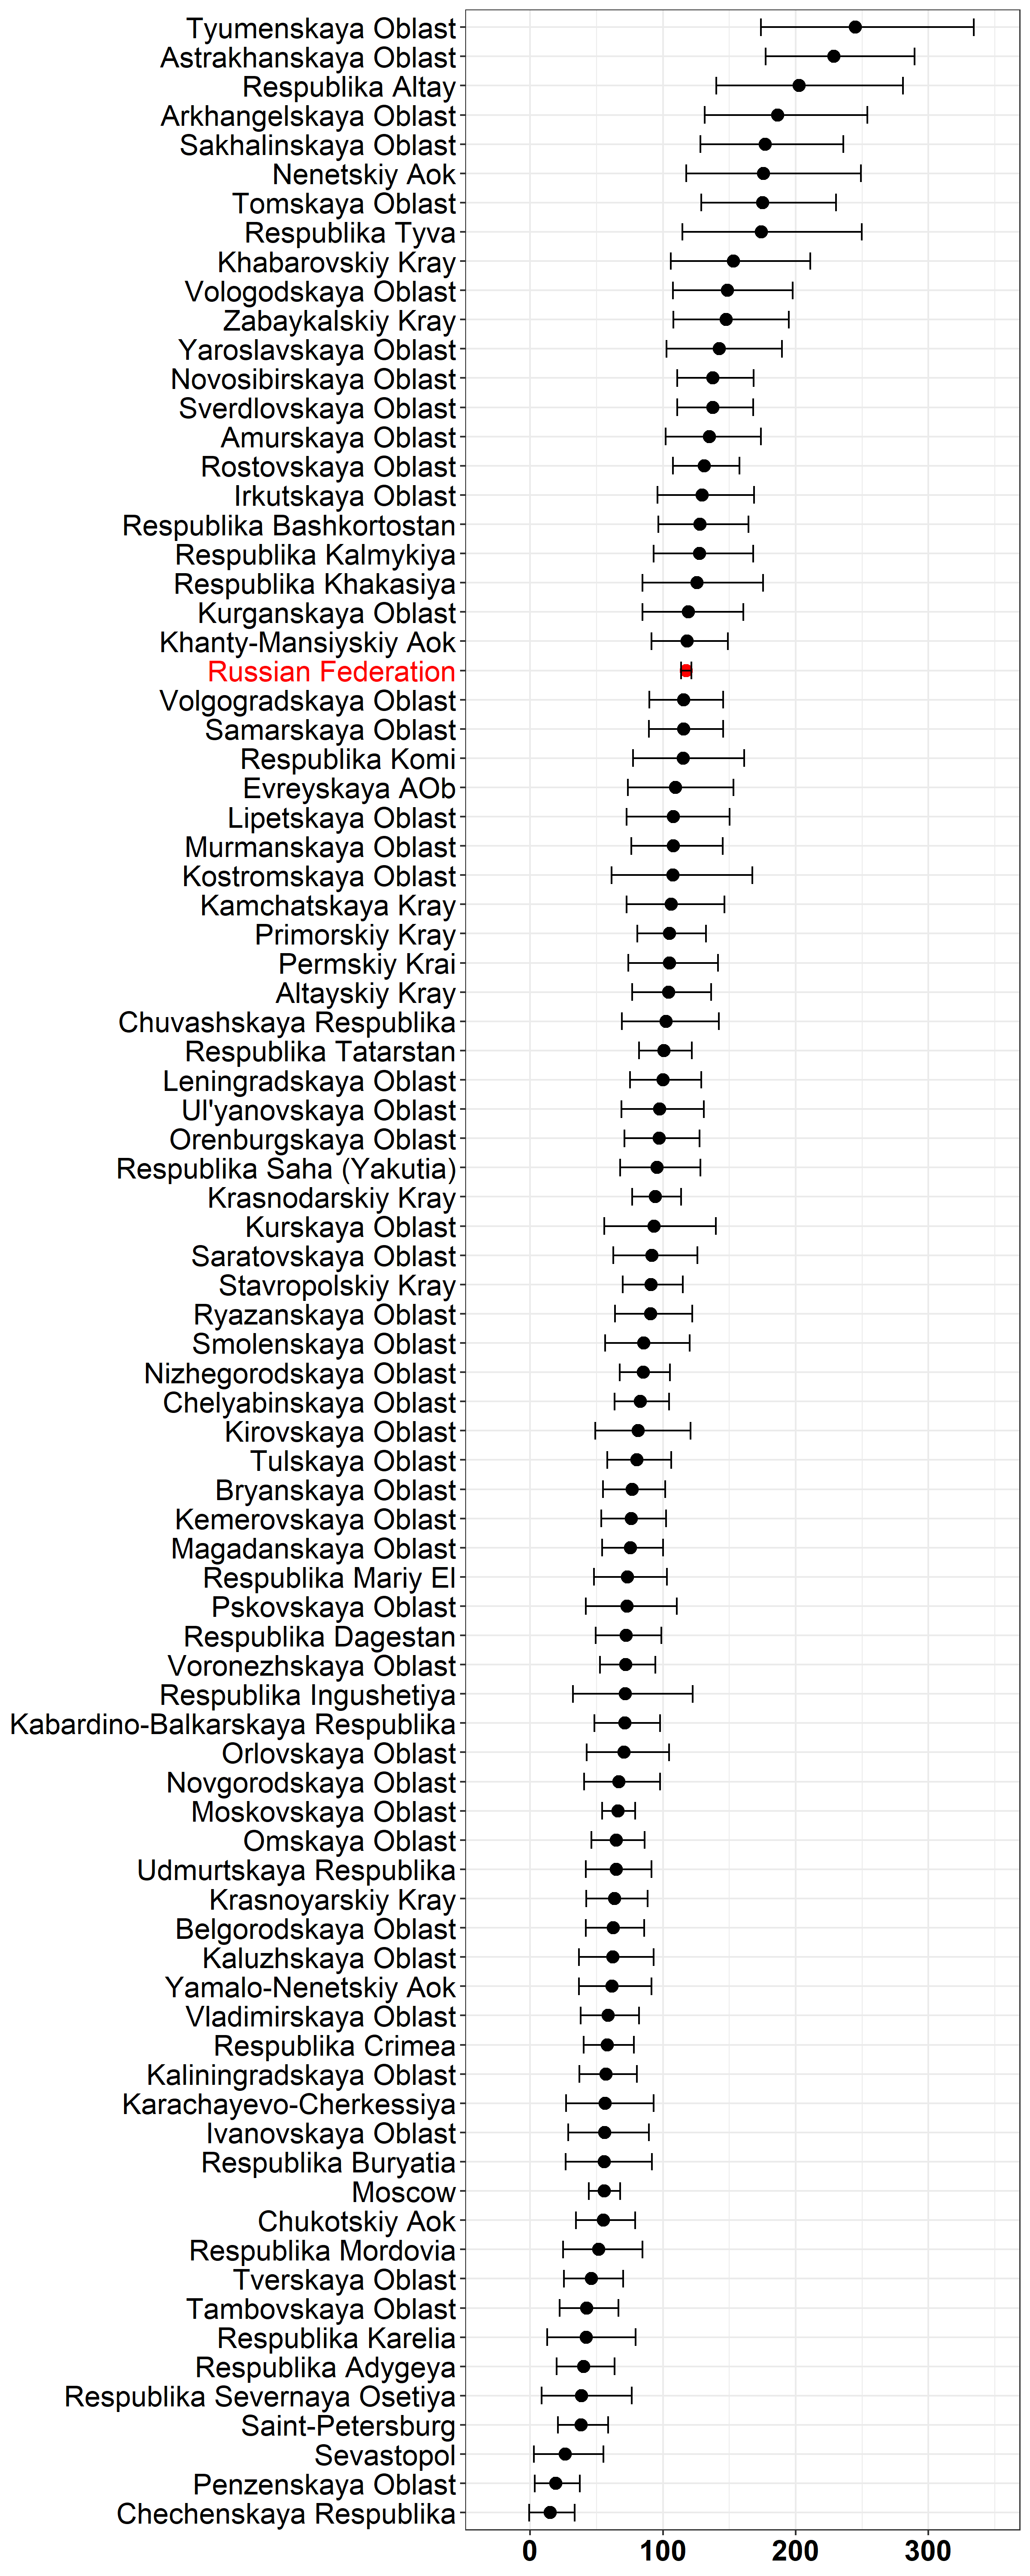
\includegraphics[width=250pt]{reg_he_18.png}
		% plot 1
		\subcaption{Higher Education}\label{}
	\end{minipage}
	\hfill
	\begin{minipage}[b]{.5\linewidth}
		\centering
		\hspace*{-0.2in}
		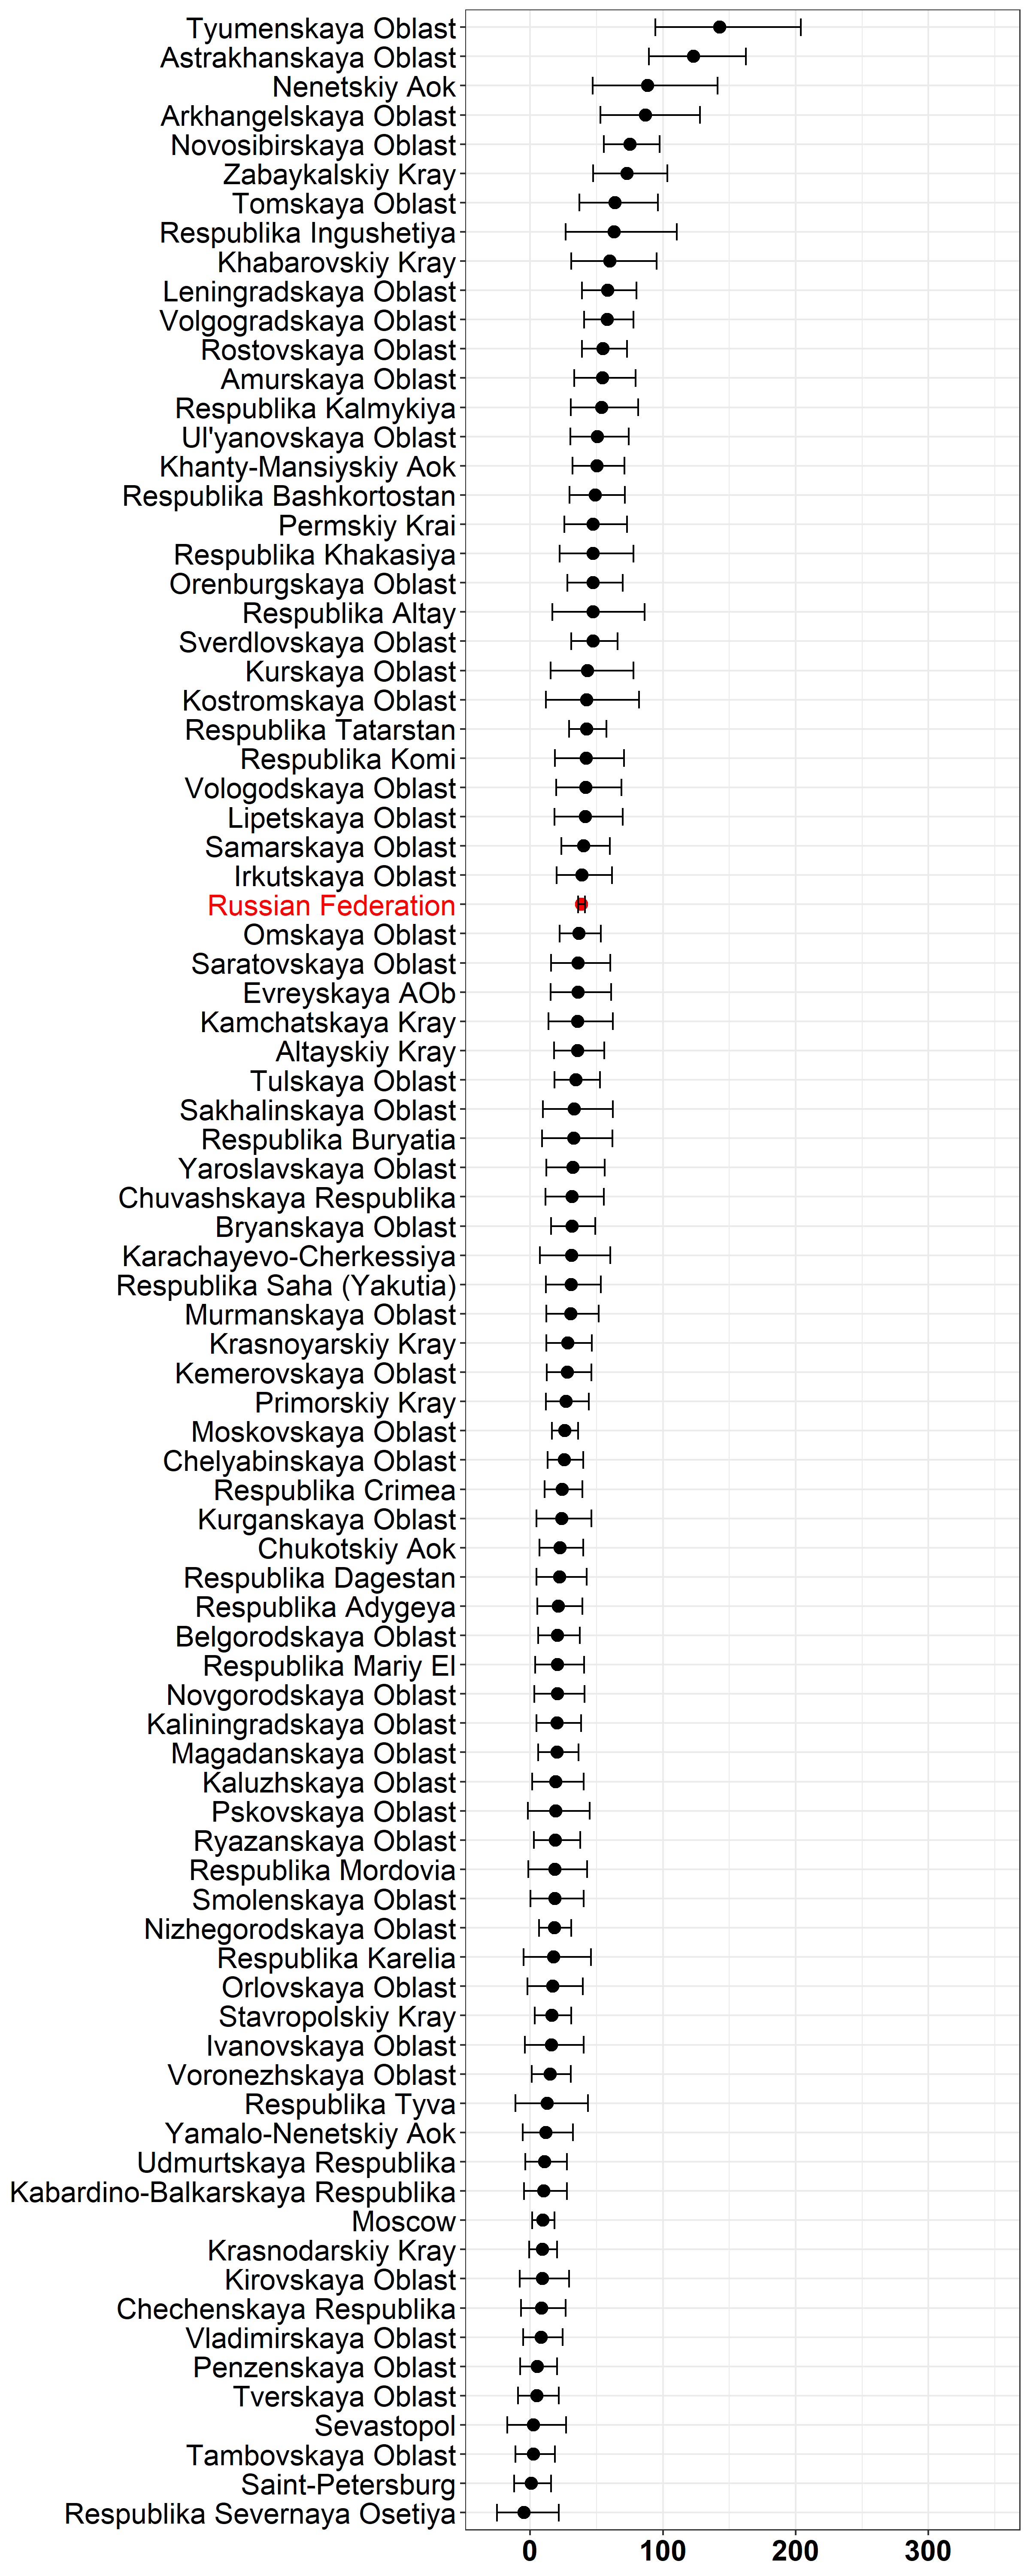
\includegraphics[width=250pt]{reg_ve_18.png}
		% plot 2
		\subcaption{Vocational Education}\label{}
	\end{minipage}
	\caption{Rates of Returns (Percentages) to Higher and Vocational Education in Russian Regions, Rosstat 2018}\label{fig:7}
\end{figure}

A two-level empty means model was initially specified and indicated that ICC was equal to 16\%, i.e., 16\% of the variation in a wage outcome was between regions, which signifies that the multilevel structure is necessary. After plugging all the predictors into the model,  a random slope for the education variable was added. Nested models comparison showed that there is a statistically significant regional variation in the effect of education on people's earnings ($-2\bigtriangleup LL(1) = 413.54, p < .001$).

Next, we examined the possible causes of this variation by adding the second-level independent variables and their interactions with education. The investigation revealed that none of the second-level characteristics are capable of changing the association between education and the amount of money Russians earn, except for \textit{the coverage by vocational education}. Substantively, it means that growth in the number of students covered by vocational programs leads to higher schooling premiums concerning both vocational and university education. As for the estimates obtained, sufficiently high vocational education coverage degree (when its standardized version is 1) corresponds to the average return rate of 30.6\%; medium vocational education coverage degree (when its standardized version is 0) corresponds to the average return rate of 35.8\%; low vocational education coverage degree (when its standardized version is -1) corresponds to the average return rate of 25.5\%. The interpretation of such a finding can imply that this quantity-related dimension of vocational education has the potential to serve as an instrument of boosting financial payoffs from post-secondary education in Russian regions.

Although the outcomes on regional examination did not establish a whole lot of associations, the empirical work conducted remains an essential step in deepening our knowledge about returns to human capital in the Russian Federation.
 
\printbibliography

\newpage
\section{Appendix}

\begin{table}[!htbp] \centering 
	\caption{Results of Multilevel Modeling with Coverage by Vocational Education, Rosstat 2018} 
	\label{} 
	\begin{tabular}{@{\extracolsep{5pt}}lcccc} 
		\\[-1.8ex]\hline 
		\hline \\[-1.8ex] 
		& Null model & Mincerian & Random Slope & Cross-Level Interaction \\ 
		\\[-1.8ex] & (1) & (2) & (3) & (4)\\ 
		\hline \\[-1.8ex] 
		Constant & 10.178$^{***}$ & 10.032$^{***}$ & 10.056$^{***}$ & 10.065$^{***}$ \\ 
		& (0.034) & (0.034) & (0.036) & (0.036) \\ 
		& & & & \\ 
		Vocational &  & 0.283$^{***}$ & 0.279$^{***}$ & 0.267$^{***}$ \\ 
		&  & (0.009) & (0.021) & (0.021) \\ 
		& & & & \\ 
		Higher &  & 0.638$^{***}$ & 0.641$^{***}$ & 0.622$^{***}$ \\ 
		&  & (0.009) & (0.025) & (0.025) \\ 
		& & & & \\ 
		Coverage VE X Vocational &  &  &  & 0.050$^{**}$ \\ 
		&  &  &  & (0.025) \\ 
		& & & & \\ 
		Coverage VE X Higher &  &  &  & 0.083$^{***}$ \\ 
		&  &  &  & (0.030) \\ 
		& & & & \\ 
		Experience &  & $-$0.026$^{***}$ & $-$0.027$^{***}$ & $-$0.027$^{***}$ \\ 
		&  & (0.002) & (0.002) & (0.002) \\ 
		& & & & \\ 
		Experience squared &  & $-$0.065$^{***}$ & $-$0.065$^{***}$ & $-$0.065$^{***}$ \\ 
		&  & (0.002) & (0.002) & (0.002) \\ 
		& & & & \\ 
		Females &  & $-$0.403$^{***}$ & $-$0.404$^{***}$ & $-$0.404$^{***}$ \\ 
		&  & (0.005) & (0.005) & (0.005) \\ 
		& & & & \\ 
		Coverage VE &  &  & $-$0.101$^{***}$ & $-$0.142$^{***}$ \\ 
		&  &  & (0.039) & (0.043) \\ 
		& & & & \\ 
		\hline
		\hline
		Variance of Intecept & 0.09 & 0.08 & 0.09 & 0.09 \\ 
		Variance of Vocational &  &  & 0.02 & 0.02 \\ 
		Variance of Higher &  &  & 0.04 & 0.04 \\ 
		Residual Deviance & 0.45 & 0.35 & 0.34 & 0.34 \\ 
		\hline
		\hline
		Observations & 49,187 & 49,187 & 49,187 & 49,187 \\ 
		Log Likelihood & $-$59,755.060 & $-$53,289.500 & $-$53,094.620 & $-$53,096.640 \\ 
		Akaike Inf. Crit. & 119,516.100 & 106,595.000 & 106,217.200 & 106,225.300 \\ 
		Bayesian Inf. Crit. & 119,542.500 & 106,665.400 & 106,340.500 & 106,366.100 \\ 
		\hline 
		\hline \\[-1.8ex] 
		\textit{Note:}  & \multicolumn{4}{r}{$^{*}$p$<$0.1; $^{**}$p$<$0.05; $^{***}$p$<$0.01} \\ 
	\end{tabular} 
\end{table} 

\begin{landscape}
	
	\fontsize{9}{11}
	\selectfont
	
	\begin{table}[!htbp] \centering 
		\caption{Results of Mincer Analysis, RLMS 1994} 
		\label{} 
		\begin{tabular}{@{\extracolsep{5pt}}lcccccc} 
			\\[-1.8ex]\hline 
			\hline \\[-1.8ex] 
			& Total & Males & Females & Total & Males & Females \\ 
			\\[-1.8ex] & (1) & (2) & (3) & (4) & (5) & (6)\\ 
			\hline \\[-1.8ex] 
			Constant & 10.892$^{***}$ & 10.974$^{***}$ & 10.319$^{***}$ & 11.777$^{***}$ & 11.947$^{***}$ & 11.132$^{***}$ \\ 
			& (10.632, 11.152) & (10.578, 11.369) & (9.979, 10.659) & (11.598, 11.957) & (11.673, 12.222) & (10.901, 11.362) \\ 
			& & & & & & \\ 
			Education, years & 0.087$^{***}$ & 0.094$^{***}$ & 0.082$^{***}$ &  &  &  \\ 
			& (0.073, 0.101) & (0.072, 0.115) & (0.063, 0.101) &  &  &  \\ 
			& & & & & & \\ 
			Vocational education &  &  &  & 0.142$^{***}$ & 0.135$^{**}$ & 0.156$^{***}$ \\ 
			&  &  &  & (0.060, 0.225) & (0.011, 0.260) & (0.046, 0.266) \\ 
			& & & & & & \\ 
			Higher education &  &  &  & 0.518$^{***}$ & 0.549$^{***}$ & 0.501$^{***}$ \\ 
			&  &  &  & (0.424, 0.611) & (0.407, 0.691) & (0.378, 0.625) \\ 
			& & & & & & \\ 
			Experience & 0.034$^{***}$ & 0.023$^{*}$ & 0.043$^{***}$ & 0.036$^{***}$ & 0.024$^{**}$ & 0.045$^{***}$ \\ 
			& (0.020, 0.049) & ($-$0.0002, 0.046) & (0.024, 0.062) & (0.021, 0.051) & (0.0005, 0.047) & (0.026, 0.065) \\ 
			& & & & & & \\ 
			Experience squared & $-$0.001$^{***}$ & $-$0.001$^{**}$ & $-$0.001$^{***}$ & $-$0.001$^{***}$ & $-$0.001$^{**}$ & $-$0.001$^{***}$ \\ 
			& ($-$0.001, $-$0.0004) & ($-$0.001, $-$0.0001) & ($-$0.001, $-$0.0004) & ($-$0.001, $-$0.0004) & ($-$0.001, $-$0.0001) & ($-$0.001, $-$0.0005) \\ 
			& & & & & & \\ 
			Female & $-$0.501$^{***}$ &  &  & $-$0.499$^{***}$ &  &  \\ 
			& ($-$0.565, $-$0.436) &  &  & ($-$0.564, $-$0.435) &  &  \\ 
			& & & & & & \\ 
			\hline \\[-1.8ex] 
			Observations & 3,044 & 1,397 & 1,647 & 3,044 & 1,397 & 1,647 \\ 
			R$^{2}$ & 0.110 & 0.055 & 0.050 & 0.109 & 0.052 & 0.049 \\ 
			Adjusted R$^{2}$ & 0.109 & 0.053 & 0.048 & 0.107 & 0.049 & 0.047 \\ 
			Residual Std. Error & 0.901 & 0.952 & 0.854 & 0.902 & 0.954 & 0.854 \\ 
			F Statistic & 94.102$^{***}$ & 27.011$^{***}$ & 28.581$^{***}$ & 73.949$^{***}$ & 19.011$^{***}$ & 21.376$^{***}$ \\ 
			\hline 
			\hline \\[-1.8ex] 
			\textit{Note:}  & \multicolumn{6}{r}{$^{*}$p$<$0.1; $^{**}$p$<$0.05; $^{***}$p$<$0.01} \\ 
		\end{tabular} 
	\end{table} 
	
\end{landscape}

\newpage

\begin{landscape}
	
	\fontsize{9}{11}
	\selectfont
	
	\begin{table}[!htbp] \centering 
		\caption{Results of Mincer Analysis, RLMS 1995} 
		\label{} 
		\begin{tabular}{@{\extracolsep{5pt}}lcccccc} 
			\\[-1.8ex]\hline 
			\hline \\[-1.8ex] 
			& Total & Males & Females & Total & Males & Females \\ 
			\\[-1.8ex] & (1) & (2) & (3) & (4) & (5) & (6)\\ 
			\hline \\[-1.8ex] 
			Constant & 11.708$^{***}$ & 12.079$^{***}$ & 10.920$^{***}$ & 12.540$^{***}$ & 12.844$^{***}$ & 11.835$^{***}$ \\ 
			& (11.433, 11.984) & (11.674, 12.484) & (10.548, 11.291) & (12.354, 12.727) & (12.566, 13.121) & (11.587, 12.082) \\ 
			& & & & & & \\ 
			Education, years & 0.080$^{***}$ & 0.073$^{***}$ & 0.089$^{***}$ &  &  &  \\ 
			& (0.065, 0.095) & (0.050, 0.096) & (0.068, 0.109) &  &  &  \\ 
			& & & & & & \\ 
			Vocational education &  &  &  & 0.085$^{*}$ & 0.062 & 0.111$^{*}$ \\ 
			&  &  &  & ($-$0.002, 0.172) & ($-$0.067, 0.190) & ($-$0.009, 0.230) \\ 
			& & & & & & \\ 
			Higher education &  &  &  & 0.442$^{***}$ & 0.393$^{***}$ & 0.498$^{***}$ \\ 
			&  &  &  & (0.346, 0.539) & (0.251, 0.534) & (0.366, 0.631) \\ 
			& & & & & & \\ 
			Experience & 0.033$^{***}$ & 0.010 & 0.053$^{***}$ & 0.035$^{***}$ & 0.012 & 0.055$^{***}$ \\ 
			& (0.018, 0.048) & ($-$0.013, 0.033) & (0.032, 0.073) & (0.020, 0.051) & ($-$0.011, 0.035) & (0.034, 0.075) \\ 
			& & & & & & \\ 
			Experience squared & $-$0.001$^{***}$ & $-$0.0003 & $-$0.001$^{***}$ & $-$0.001$^{***}$ & $-$0.0004 & $-$0.001$^{***}$ \\ 
			& ($-$0.001, $-$0.0004) & ($-$0.001, 0.0002) & ($-$0.001, $-$0.001) & ($-$0.001, $-$0.0004) & ($-$0.001, 0.0001) & ($-$0.002, $-$0.001) \\ 
			& & & & & & \\ 
			Female & $-$0.439$^{***}$ &  &  & $-$0.437$^{***}$ &  &  \\ 
			& ($-$0.506, $-$0.371) &  &  & ($-$0.505, $-$0.369) &  &  \\ 
			& & & & & & \\ 
			\hline \\[-1.8ex] 
			Observations & 2,694 & 1,238 & 1,456 & 2,694 & 1,238 & 1,456 \\ 
			R$^{2}$ & 0.093 & 0.036 & 0.057 & 0.093 & 0.036 & 0.058 \\ 
			Adjusted R$^{2}$ & 0.091 & 0.034 & 0.055 & 0.091 & 0.033 & 0.055 \\ 
			Residual Std. Error & 0.893 & 0.920 & 0.866 & 0.893 & 0.920 & 0.866 \\ 
			F Statistic & 68.547$^{***}$ & 15.338$^{***}$ & 29.289$^{***}$ & 54.958$^{***}$ & 11.401$^{***}$ & 22.178$^{***}$ \\ 
			\hline 
			\hline \\[-1.8ex] 
			\textit{Note:}  & \multicolumn{6}{r}{$^{*}$p$<$0.1; $^{**}$p$<$0.05; $^{***}$p$<$0.01} \\ 
		\end{tabular} 
	\end{table} 
	
\end{landscape}

\newpage

\begin{landscape}
	
	\fontsize{9}{11}
	\selectfont
	
	\begin{table}[!htbp] \centering 
		\caption{Results of Mincer Analysis, RLMS 1996} 
		\label{} 
		\begin{tabular}{@{\extracolsep{5pt}}lcccccc} 
			\\[-1.8ex]\hline 
			\hline \\[-1.8ex] 
			& Total & Males & Females & Total & Males & Females \\ 
			\\[-1.8ex] & (1) & (2) & (3) & (4) & (5) & (6)\\ 
			\hline \\[-1.8ex] 
			Constant & 12.412$^{***}$ & 12.539$^{***}$ & 11.814$^{***}$ & 13.167$^{***}$ & 13.306$^{***}$ & 12.568$^{***}$ \\ 
			& (12.100, 12.725) & (12.066, 13.013) & (11.401, 12.227) & (12.956, 13.378) & (12.987, 13.625) & (12.292, 12.843) \\ 
			& & & & & & \\ 
			Education, years & 0.075$^{***}$ & 0.076$^{***}$ & 0.074$^{***}$ &  &  &  \\ 
			& (0.057, 0.092) & (0.049, 0.103) & (0.051, 0.098) &  &  &  \\ 
			& & & & & & \\ 
			Vocational education &  &  &  & 0.127$^{**}$ & 0.130 & 0.126$^{*}$ \\ 
			&  &  &  & (0.025, 0.230) & ($-$0.026, 0.286) & ($-$0.010, 0.261) \\ 
			& & & & & & \\ 
			Higher education &  &  &  & 0.407$^{***}$ & 0.403$^{***}$ & 0.412$^{***}$ \\ 
			&  &  &  & (0.295, 0.519) & (0.232, 0.574) & (0.265, 0.560) \\ 
			& & & & & & \\ 
			Experience & 0.009 & $-$0.001 & 0.018 & 0.011 & 0.001 & 0.019$^{*}$ \\ 
			& ($-$0.008, 0.026) & ($-$0.027, 0.025) & ($-$0.005, 0.040) & ($-$0.006, 0.028) & ($-$0.025, 0.027) & ($-$0.003, 0.042) \\ 
			& & & & & & \\ 
			Experience squared & $-$0.0003 & $-$0.0001 & $-$0.0004 & $-$0.0003$^{*}$ & $-$0.0002 & $-$0.0004$^{*}$ \\ 
			& ($-$0.001, 0.0001) & ($-$0.001, 0.0004) & ($-$0.001, 0.0001) & ($-$0.001, 0.00005) & ($-$0.001, 0.0004) & ($-$0.001, 0.0001) \\ 
			& & & & & & \\ 
			Female & $-$0.483$^{***}$ &  &  & $-$0.480$^{***}$ &  &  \\ 
			& ($-$0.559, $-$0.406) &  &  & ($-$0.556, $-$0.403) &  &  \\ 
			& & & & & & \\ 
			\hline \\[-1.8ex] 
			Observations & 2,282 & 1,034 & 1,248 & 2,282 & 1,034 & 1,248 \\ 
			R$^{2}$ & 0.090 & 0.037 & 0.033 & 0.086 & 0.032 & 0.031 \\ 
			Adjusted R$^{2}$ & 0.088 & 0.035 & 0.031 & 0.084 & 0.028 & 0.028 \\ 
			Residual Std. Error & 0.927 & 0.974 & 0.886 & 0.929 & 0.977 & 0.887 \\ 
			F Statistic & 56.097$^{***}$ & 13.324$^{***}$ & 14.098$^{***}$ & 43.041$^{***}$ & 8.574$^{***}$ & 9.880$^{***}$ \\ 
			\hline 
			\hline \\[-1.8ex] 
			\textit{Note:}  & \multicolumn{6}{r}{$^{*}$p$<$0.1; $^{**}$p$<$0.05; $^{***}$p$<$0.01} \\ 
		\end{tabular} 
	\end{table} 
	
\end{landscape}

\newpage

\begin{landscape}
	
	\fontsize{9}{11}
	\selectfont
	
	\begin{table}[!htbp] \centering 
		\caption{Results of Mincer Analysis, RLMS 1998} 
		\label{} 
		\begin{tabular}{@{\extracolsep{5pt}}lcccccc} 
			\\[-1.8ex]\hline 
			\hline \\[-1.8ex] 
			& Total & Males & Females & Total & Males & Females \\ 
			\\[-1.8ex] & (1) & (2) & (3) & (4) & (5) & (6)\\ 
			\hline \\[-1.8ex] 
			Constant & 5.219$^{***}$ & 5.425$^{***}$ & 4.564$^{***}$ & 6.139$^{***}$ & 6.338$^{***}$ & 5.502$^{***}$ \\ 
			& (4.997, 5.442) & (5.090, 5.760) & (4.267, 4.861) & (5.987, 6.291) & (6.106, 6.571) & (5.303, 5.700) \\ 
			& & & & & & \\ 
			Education, years & 0.097$^{***}$ & 0.095$^{***}$ & 0.099$^{***}$ &  &  &  \\ 
			& (0.084, 0.109) & (0.076, 0.114) & (0.083, 0.116) &  &  &  \\ 
			& & & & & & \\ 
			Vocational education &  &  &  & 0.214$^{***}$ & 0.175$^{***}$ & 0.257$^{***}$ \\ 
			&  &  &  & (0.143, 0.286) & (0.070, 0.280) & (0.158, 0.355) \\ 
			& & & & & & \\ 
			Higher education &  &  &  & 0.581$^{***}$ & 0.556$^{***}$ & 0.615$^{***}$ \\ 
			&  &  &  & (0.500, 0.662) & (0.435, 0.677) & (0.506, 0.725) \\ 
			& & & & & & \\ 
			Experience & 0.029$^{***}$ & 0.013 & 0.041$^{***}$ & 0.032$^{***}$ & 0.018$^{*}$ & 0.043$^{***}$ \\ 
			& (0.017, 0.041) & ($-$0.005, 0.032) & (0.025, 0.057) & (0.020, 0.044) & ($-$0.001, 0.037) & (0.027, 0.059) \\ 
			& & & & & & \\ 
			Experience squared & $-$0.001$^{***}$ & $-$0.0004$^{*}$ & $-$0.001$^{***}$ & $-$0.001$^{***}$ & $-$0.0005$^{**}$ & $-$0.001$^{***}$ \\ 
			& ($-$0.001, $-$0.0004) & ($-$0.001, 0.00003) & ($-$0.001, $-$0.001) & ($-$0.001, $-$0.0004) & ($-$0.001, $-$0.0001) & ($-$0.001, $-$0.001) \\ 
			& & & & & & \\ 
			Female & $-$0.476$^{***}$ &  &  & $-$0.471$^{***}$ &  &  \\ 
			& ($-$0.530, $-$0.422) &  &  & ($-$0.525, $-$0.416) &  &  \\ 
			& & & & & & \\ 
			\hline \\[-1.8ex] 
			Observations & 3,102 & 1,434 & 1,668 & 3,102 & 1,434 & 1,668 \\ 
			R$^{2}$ & 0.139 & 0.069 & 0.085 & 0.138 & 0.067 & 0.085 \\ 
			Adjusted R$^{2}$ & 0.138 & 0.067 & 0.083 & 0.137 & 0.064 & 0.083 \\ 
			Residual Std. Error & 0.765 & 0.803 & 0.730 & 0.765 & 0.804 & 0.730 \\ 
			F Statistic & 125.414$^{***}$ & 35.348$^{***}$ & 51.380$^{***}$ & 99.388$^{***}$ & 25.536$^{***}$ & 38.668$^{***}$ \\ 
			\hline 
			\hline \\[-1.8ex] 
			\textit{Note:}  & \multicolumn{6}{r}{$^{*}$p$<$0.1; $^{**}$p$<$0.05; $^{***}$p$<$0.01} \\ 
		\end{tabular} 
	\end{table} 
	
\end{landscape}

\newpage

\begin{landscape}
	
	\fontsize{9}{11}
	\selectfont
	
	\begin{table}[!htbp] \centering 
		\caption{Results of Mincer Analysis, RLMS 2000} 
		\label{} 
		\begin{tabular}{@{\extracolsep{5pt}}lcccccc} 
			\\[-1.8ex]\hline 
			\hline \\[-1.8ex] 
			& Total & Males & Females & Total & Males & Females \\ 
			\\[-1.8ex] & (1) & (2) & (3) & (4) & (5) & (6)\\ 
			\hline \\[-1.8ex] 
			Constant & 5.920$^{***}$ & 6.311$^{***}$ & 5.023$^{***}$ & 6.887$^{***}$ & 7.183$^{***}$ & 6.072$^{***}$ \\ 
			& (5.689, 6.152) & (5.966, 6.655) & (4.710, 5.336) & (6.736, 7.038) & (6.961, 7.405) & (5.869, 6.276) \\ 
			& & & & & & \\ 
			Education, years & 0.098$^{***}$ & 0.086$^{***}$ & 0.110$^{***}$ &  &  &  \\ 
			& (0.084, 0.111) & (0.065, 0.106) & (0.092, 0.128) &  &  &  \\ 
			& & & & & & \\ 
			Vocational education &  &  &  & 0.193$^{***}$ & 0.118$^{**}$ & 0.283$^{***}$ \\ 
			&  &  &  & (0.117, 0.269) & (0.008, 0.228) & (0.178, 0.388) \\ 
			& & & & & & \\ 
			Higher education &  &  &  & 0.554$^{***}$ & 0.450$^{***}$ & 0.668$^{***}$ \\ 
			&  &  &  & (0.469, 0.640) & (0.323, 0.578) & (0.553, 0.784) \\ 
			& & & & & & \\ 
			Experience & 0.025$^{***}$ & 0.006 & 0.041$^{***}$ & 0.027$^{***}$ & 0.009 & 0.042$^{***}$ \\ 
			& (0.013, 0.037) & ($-$0.012, 0.025) & (0.024, 0.057) & (0.015, 0.039) & ($-$0.009, 0.028) & (0.025, 0.058) \\ 
			& & & & & & \\ 
			Experience squared & $-$0.001$^{***}$ & $-$0.0002 & $-$0.001$^{***}$ & $-$0.001$^{***}$ & $-$0.0003$^{*}$ & $-$0.001$^{***}$ \\ 
			& ($-$0.001, $-$0.0003) & ($-$0.001, 0.0001) & ($-$0.001, $-$0.0004) & ($-$0.001, $-$0.0003) & ($-$0.001, 0.0001) & ($-$0.001, $-$0.0005) \\ 
			& & & & & & \\ 
			Female & $-$0.538$^{***}$ &  &  & $-$0.533$^{***}$ &  &  \\ 
			& ($-$0.596, $-$0.480) &  &  & ($-$0.590, $-$0.475) &  &  \\ 
			& & & & & & \\ 
			\hline \\[-1.8ex] 
			Observations & 3,215 & 1,477 & 1,738 & 3,215 & 1,477 & 1,738 \\ 
			R$^{2}$ & 0.137 & 0.053 & 0.084 & 0.133 & 0.047 & 0.082 \\ 
			Adjusted R$^{2}$ & 0.136 & 0.051 & 0.082 & 0.131 & 0.044 & 0.080 \\ 
			Residual Std. Error & 0.825 & 0.856 & 0.796 & 0.828 & 0.859 & 0.797 \\ 
			F Statistic & 127.527$^{***}$ & 27.384$^{***}$ & 53.004$^{***}$ & 98.038$^{***}$ & 17.961$^{***}$ & 38.813$^{***}$ \\ 
			\hline 
			\hline \\[-1.8ex] 
			\textit{Note:}  & \multicolumn{6}{r}{$^{*}$p$<$0.1; $^{**}$p$<$0.05; $^{***}$p$<$0.01} \\ 
		\end{tabular} 
	\end{table} 
	
\end{landscape}

\newpage

\begin{landscape}
	
	\fontsize{9}{11}
	\selectfont
	
	\begin{table}[!htbp] \centering 
		\caption{Results of Mincer Analysis, RLMS 2001} 
		\label{} 
		\begin{tabular}{@{\extracolsep{5pt}}lcccccc} 
			\\[-1.8ex]\hline 
			\hline \\[-1.8ex] 
			& Total & Males & Females & Total & Males & Females \\ 
			\\[-1.8ex] & (1) & (2) & (3) & (4) & (5) & (6)\\ 
			\hline \\[-1.8ex] 
			Constant & 6.383$^{***}$ & 6.648$^{***}$ & 5.647$^{***}$ & 7.415$^{***}$ & 7.592$^{***}$ & 6.758$^{***}$ \\ 
			& (6.168, 6.598) & (6.329, 6.968) & (5.355, 5.939) & (7.277, 7.554) & (7.389, 7.795) & (6.569, 6.947) \\ 
			& & & & & & \\ 
			Education, years & 0.103$^{***}$ & 0.092$^{***}$ & 0.116$^{***}$ &  &  &  \\ 
			& (0.091, 0.116) & (0.073, 0.111) & (0.099, 0.132) &  &  &  \\ 
			& & & & & & \\ 
			Vocational education &  &  &  & 0.188$^{***}$ & 0.111$^{**}$ & 0.293$^{***}$ \\ 
			&  &  &  & (0.117, 0.260) & (0.008, 0.213) & (0.193, 0.393) \\ 
			& & & & & & \\ 
			Higher education &  &  &  & 0.589$^{***}$ & 0.496$^{***}$ & 0.711$^{***}$ \\ 
			&  &  &  & (0.511, 0.668) & (0.380, 0.612) & (0.603, 0.819) \\ 
			& & & & & & \\ 
			Experience & 0.008 & 0.001 & 0.013 & 0.010 & 0.004 & 0.013 \\ 
			& ($-$0.004, 0.019) & ($-$0.016, 0.018) & ($-$0.003, 0.029) & ($-$0.002, 0.021) & ($-$0.014, 0.021) & ($-$0.003, 0.029) \\ 
			& & & & & & \\ 
			Experience squared & $-$0.0002 & $-$0.0001 & $-$0.0002 & $-$0.0002$^{*}$ & $-$0.0002 & $-$0.0002 \\ 
			& ($-$0.0004, 0.0001) & ($-$0.0005, 0.0002) & ($-$0.001, 0.0001) & ($-$0.0005, 0.00002) & ($-$0.001, 0.0002) & ($-$0.001, 0.0001) \\ 
			& & & & & & \\ 
			Female & $-$0.466$^{***}$ &  &  & $-$0.465$^{***}$ &  &  \\ 
			& ($-$0.519, $-$0.412) &  &  & ($-$0.519, $-$0.412) &  &  \\ 
			& & & & & & \\ 
			\hline \\[-1.8ex] 
			Observations & 3,605 & 1,673 & 1,932 & 3,605 & 1,673 & 1,932 \\ 
			R$^{2}$ & 0.127 & 0.060 & 0.090 & 0.126 & 0.057 & 0.092 \\ 
			Adjusted R$^{2}$ & 0.126 & 0.058 & 0.088 & 0.125 & 0.055 & 0.090 \\ 
			Residual Std. Error & 0.811 & 0.851 & 0.774 & 0.812 & 0.852 & 0.773 \\ 
			F Statistic & 131.270$^{***}$ & 35.323$^{***}$ & 63.474$^{***}$ & 103.747$^{***}$ & 25.340$^{***}$ & 48.998$^{***}$ \\ 
			\hline 
			\hline \\[-1.8ex] 
			\textit{Note:}  & \multicolumn{6}{r}{$^{*}$p$<$0.1; $^{**}$p$<$0.05; $^{***}$p$<$0.01} \\ 
		\end{tabular} 
	\end{table} 
	
\end{landscape}

\newpage

\begin{landscape}
	
	\fontsize{9}{11}
	\selectfont
	
	\begin{table}[!htbp] \centering 
		\caption{Results of Mincer Analysis, RLMS 2002} 
		\label{} 
		\begin{tabular}{@{\extracolsep{5pt}}lcccccc} 
			\\[-1.8ex]\hline 
			\hline \\[-1.8ex] 
			& Total & Males & Females & Total & Males & Females \\ 
			\\[-1.8ex] & (1) & (2) & (3) & (4) & (5) & (6)\\ 
			\hline \\[-1.8ex] 
			Constant & 6.584$^{***}$ & 6.852$^{***}$ & 5.884$^{***}$ & 7.597$^{***}$ & 7.795$^{***}$ & 6.957$^{***}$ \\ 
			& (6.391, 6.777) & (6.567, 7.137) & (5.620, 6.147) & (7.472, 7.722) & (7.614, 7.976) & (6.785, 7.129) \\ 
			& & & & & & \\ 
			Education, years & 0.103$^{***}$ & 0.093$^{***}$ & 0.113$^{***}$ &  &  &  \\ 
			& (0.092, 0.114) & (0.076, 0.111) & (0.098, 0.128) &  &  &  \\ 
			& & & & & & \\ 
			Vocational education &  &  &  & 0.192$^{***}$ & 0.120$^{**}$ & 0.283$^{***}$ \\ 
			&  &  &  & (0.128, 0.257) & (0.028, 0.211) & (0.192, 0.374) \\ 
			& & & & & & \\ 
			Higher education &  &  &  & 0.582$^{***}$ & 0.498$^{***}$ & 0.686$^{***}$ \\ 
			&  &  &  & (0.511, 0.653) & (0.394, 0.602) & (0.588, 0.784) \\ 
			& & & & & & \\ 
			Experience & 0.021$^{***}$ & 0.012 & 0.028$^{***}$ & 0.024$^{***}$ & 0.016$^{**}$ & 0.029$^{***}$ \\ 
			& (0.011, 0.032) & ($-$0.003, 0.028) & (0.014, 0.042) & (0.013, 0.034) & (0.001, 0.032) & (0.014, 0.043) \\ 
			& & & & & & \\ 
			Experience squared & $-$0.0004$^{***}$ & $-$0.0004$^{**}$ & $-$0.0005$^{***}$ & $-$0.001$^{***}$ & $-$0.0005$^{***}$ & $-$0.0005$^{***}$ \\ 
			& ($-$0.001, $-$0.0002) & ($-$0.001, $-$0.0001) & ($-$0.001, $-$0.0002) & ($-$0.001, $-$0.0003) & ($-$0.001, $-$0.0001) & ($-$0.001, $-$0.0002) \\ 
			& & & & & & \\ 
			Female & $-$0.443$^{***}$ &  &  & $-$0.442$^{***}$ &  &  \\ 
			& ($-$0.491, $-$0.396) &  &  & ($-$0.490, $-$0.394) &  &  \\ 
			& & & & & & \\ 
			\hline \\[-1.8ex] 
			Observations & 3,803 & 1,748 & 2,055 & 3,803 & 1,748 & 2,055 \\ 
			R$^{2}$ & 0.137 & 0.072 & 0.098 & 0.134 & 0.068 & 0.099 \\ 
			Adjusted R$^{2}$ & 0.136 & 0.071 & 0.097 & 0.133 & 0.066 & 0.097 \\ 
			Residual Std. Error & 0.746 & 0.770 & 0.722 & 0.747 & 0.771 & 0.722 \\ 
			F Statistic & 150.882$^{***}$ & 45.377$^{***}$ & 74.224$^{***}$ & 117.987$^{***}$ & 31.968$^{***}$ & 56.066$^{***}$ \\ 
			\hline 
			\hline \\[-1.8ex] 
			\textit{Note:}  & \multicolumn{6}{r}{$^{*}$p$<$0.1; $^{**}$p$<$0.05; $^{***}$p$<$0.01} \\ 
		\end{tabular} 
	\end{table} 
	
\end{landscape}

\newpage

\begin{landscape}
	
	\fontsize{9}{11}
	\selectfont
	
	\begin{table}[!htbp] \centering 
		\caption{Results of Mincer Analysis, RLMS 2003} 
		\label{} 
		\begin{tabular}{@{\extracolsep{5pt}}lcccccc} 
			\\[-1.8ex]\hline 
			\hline \\[-1.8ex] 
			& Total & Males & Females & Total & Males & Females \\ 
			\\[-1.8ex] & (1) & (2) & (3) & (4) & (5) & (6)\\ 
			\hline \\[-1.8ex] 
			Constant & 6.862$^{***}$ & 7.204$^{***}$ & 6.054$^{***}$ & 7.887$^{***}$ & 8.127$^{***}$ & 7.167$^{***}$ \\ 
			& (6.671, 7.053) & (6.922, 7.486) & (5.793, 6.315) & (7.763, 8.011) & (7.945, 8.308) & (7.001, 7.333) \\ 
			& & & & & & \\ 
			Education, years & 0.104$^{***}$ & 0.089$^{***}$ & 0.119$^{***}$ &  &  &  \\ 
			& (0.093, 0.116) & (0.073, 0.106) & (0.104, 0.134) &  &  &  \\ 
			& & & & & & \\ 
			Vocational education &  &  &  & 0.209$^{***}$ & 0.114$^{**}$ & 0.323$^{***}$ \\ 
			&  &  &  & (0.144, 0.273) & (0.023, 0.204) & (0.232, 0.414) \\ 
			& & & & & & \\ 
			Higher education &  &  &  & 0.590$^{***}$ & 0.456$^{***}$ & 0.740$^{***}$ \\ 
			&  &  &  & (0.519, 0.661) & (0.353, 0.558) & (0.642, 0.838) \\ 
			& & & & & & \\ 
			Experience & 0.018$^{***}$ & 0.009 & 0.025$^{***}$ & 0.020$^{***}$ & 0.011 & 0.025$^{***}$ \\ 
			& (0.007, 0.028) & ($-$0.007, 0.024) & (0.011, 0.038) & (0.009, 0.030) & ($-$0.005, 0.027) & (0.011, 0.039) \\ 
			& & & & & & \\ 
			Experience squared & $-$0.0004$^{***}$ & $-$0.0004$^{**}$ & $-$0.0005$^{***}$ & $-$0.0005$^{***}$ & $-$0.0004$^{**}$ & $-$0.0005$^{***}$ \\ 
			& ($-$0.001, $-$0.0002) & ($-$0.001, $-$0.00002) & ($-$0.001, $-$0.0002) & ($-$0.001, $-$0.0002) & ($-$0.001, $-$0.0001) & ($-$0.001, $-$0.0002) \\ 
			& & & & & & \\ 
			Female & $-$0.491$^{***}$ &  &  & $-$0.485$^{***}$ &  &  \\ 
			& ($-$0.538, $-$0.444) &  &  & ($-$0.533, $-$0.438) &  &  \\ 
			& & & & & & \\ 
			\hline \\[-1.8ex] 
			Observations & 3,858 & 1,765 & 2,093 & 3,858 & 1,765 & 2,093 \\ 
			R$^{2}$ & 0.158 & 0.078 & 0.107 & 0.153 & 0.069 & 0.110 \\ 
			Adjusted R$^{2}$ & 0.157 & 0.077 & 0.106 & 0.152 & 0.067 & 0.108 \\ 
			Residual Std. Error & 0.743 & 0.753 & 0.732 & 0.746 & 0.757 & 0.731 \\ 
			F Statistic & 180.727$^{***}$ & 49.918$^{***}$ & 83.800$^{***}$ & 139.128$^{***}$ & 32.690$^{***}$ & 64.384$^{***}$ \\ 
			\hline 
			\hline \\[-1.8ex] 
			\textit{Note:}  & \multicolumn{6}{r}{$^{*}$p$<$0.1; $^{**}$p$<$0.05; $^{***}$p$<$0.01} \\ 
		\end{tabular} 
	\end{table} 
	
\end{landscape}

\newpage

\begin{landscape}
	
	\fontsize{9}{11}
	\selectfont
	
	\begin{table}[!htbp] \centering 
		\caption{Results of Mincer Analysis, RLMS 2004} 
		\label{} 
		\begin{tabular}{@{\extracolsep{5pt}}lcccccc} 
			\\[-1.8ex]\hline 
			\hline \\[-1.8ex] 
			& Total & Males & Females & Total & Males & Females \\ 
			\\[-1.8ex] & (1) & (2) & (3) & (4) & (5) & (6)\\ 
			\hline \\[-1.8ex] 
			Constant & 7.235$^{***}$ & 7.559$^{***}$ & 6.437$^{***}$ & 8.216$^{***}$ & 8.404$^{***}$ & 7.553$^{***}$ \\ 
			& (7.054, 7.415) & (7.293, 7.825) & (6.191, 6.683) & (8.100, 8.332) & (8.233, 8.574) & (7.397, 7.710) \\ 
			& & & & & & \\ 
			Education, years & 0.097$^{***}$ & 0.084$^{***}$ & 0.111$^{***}$ &  &  &  \\ 
			& (0.087, 0.108) & (0.068, 0.099) & (0.097, 0.125) &  &  &  \\ 
			& & & & & & \\ 
			Vocational education &  &  &  & 0.151$^{***}$ & 0.135$^{***}$ & 0.180$^{***}$ \\ 
			&  &  &  & (0.090, 0.212) & (0.050, 0.221) & (0.093, 0.267) \\ 
			& & & & & & \\ 
			Higher education &  &  &  & 0.525$^{***}$ & 0.443$^{***}$ & 0.610$^{***}$ \\ 
			&  &  &  & (0.458, 0.593) & (0.345, 0.540) & (0.516, 0.704) \\ 
			& & & & & & \\ 
			Experience & 0.015$^{***}$ & 0.005 & 0.022$^{***}$ & 0.018$^{***}$ & 0.007 & 0.024$^{***}$ \\ 
			& (0.006, 0.025) & ($-$0.009, 0.020) & (0.009, 0.035) & (0.008, 0.027) & ($-$0.007, 0.022) & (0.011, 0.038) \\ 
			& & & & & & \\ 
			Experience squared & $-$0.0004$^{***}$ & $-$0.0003$^{*}$ & $-$0.0005$^{***}$ & $-$0.0005$^{***}$ & $-$0.0004$^{**}$ & $-$0.001$^{***}$ \\ 
			& ($-$0.001, $-$0.0002) & ($-$0.001, 0.00000) & ($-$0.001, $-$0.0002) & ($-$0.001, $-$0.0003) & ($-$0.001, $-$0.00005) & ($-$0.001, $-$0.0002) \\ 
			& & & & & & \\ 
			Female & $-$0.498$^{***}$ &  &  & $-$0.494$^{***}$ &  &  \\ 
			& ($-$0.543, $-$0.454) &  &  & ($-$0.538, $-$0.449) &  &  \\ 
			& & & & & & \\ 
			\hline \\[-1.8ex] 
			Observations & 3,968 & 1,824 & 2,144 & 3,968 & 1,824 & 2,144 \\ 
			R$^{2}$ & 0.170 & 0.084 & 0.106 & 0.162 & 0.075 & 0.101 \\ 
			Adjusted R$^{2}$ & 0.169 & 0.083 & 0.105 & 0.161 & 0.073 & 0.099 \\ 
			Residual Std. Error & 0.706 & 0.720 & 0.690 & 0.709 & 0.724 & 0.693 \\ 
			F Statistic & 202.301$^{***}$ & 55.701$^{***}$ & 84.918$^{***}$ & 153.588$^{***}$ & 36.626$^{***}$ & 59.781$^{***}$ \\ 
			\hline 
			\hline \\[-1.8ex] 
			\textit{Note:}  & \multicolumn{6}{r}{$^{*}$p$<$0.1; $^{**}$p$<$0.05; $^{***}$p$<$0.01} \\ 
		\end{tabular} 
	\end{table} 
	
\end{landscape}

\newpage

\begin{landscape}
	
	\fontsize{9}{11}
	\selectfont
	
	\begin{table}[!htbp] \centering 
		\caption{Results of Mincer Analysis, RLMS 2005} 
		\label{} 
		\begin{tabular}{@{\extracolsep{5pt}}lcccccc} 
			\\[-1.8ex]\hline 
			\hline \\[-1.8ex] 
			& Total & Males & Females & Total & Males & Females \\ 
			\\[-1.8ex] & (1) & (2) & (3) & (4) & (5) & (6)\\ 
			\hline \\[-1.8ex] 
			Constant & 7.585$^{***}$ & 7.969$^{***}$ & 6.729$^{***}$ & 8.543$^{***}$ & 8.722$^{***}$ & 7.868$^{***}$ \\ 
			& (7.406, 7.764) & (7.703, 8.235) & (6.485, 6.972) & (8.430, 8.657) & (8.555, 8.890) & (7.715, 8.021) \\ 
			& & & & & & \\ 
			Education, years & 0.095$^{***}$ & 0.074$^{***}$ & 0.113$^{***}$ &  &  &  \\ 
			& (0.084, 0.105) & (0.059, 0.090) & (0.099, 0.127) &  &  &  \\ 
			& & & & & & \\ 
			Vocational education &  &  &  & 0.140$^{***}$ & 0.110$^{**}$ & 0.189$^{***}$ \\ 
			&  &  &  & (0.079, 0.201) & (0.026, 0.195) & (0.101, 0.277) \\ 
			& & & & & & \\ 
			Higher education &  &  &  & 0.515$^{***}$ & 0.388$^{***}$ & 0.640$^{***}$ \\ 
			&  &  &  & (0.448, 0.582) & (0.291, 0.484) & (0.546, 0.734) \\ 
			& & & & & & \\ 
			Experience & 0.005 & $-$0.004 & 0.011$^{*}$ & 0.007 & $-$0.002 & 0.013$^{**}$ \\ 
			& ($-$0.005, 0.014) & ($-$0.018, 0.010) & ($-$0.001, 0.024) & ($-$0.003, 0.016) & ($-$0.016, 0.013) & (0.0004, 0.025) \\ 
			& & & & & & \\ 
			Experience squared & $-$0.0002$^{*}$ & $-$0.0001 & $-$0.0003$^{*}$ & $-$0.0002$^{**}$ & $-$0.0001 & $-$0.0003$^{**}$ \\ 
			& ($-$0.0004, 0.00002) & ($-$0.0004, 0.0002) & ($-$0.001, 0.00001) & ($-$0.0004, $-$0.00003) & ($-$0.0004, 0.0002) & ($-$0.001, $-$0.00001) \\ 
			& & & & & & \\ 
			Female & $-$0.503$^{***}$ &  &  & $-$0.498$^{***}$ &  &  \\ 
			& ($-$0.548, $-$0.459) &  &  & ($-$0.542, $-$0.453) &  &  \\ 
			& & & & & & \\ 
			\hline \\[-1.8ex] 
			Observations & 3,913 & 1,801 & 2,112 & 3,913 & 1,801 & 2,112 \\ 
			R$^{2}$ & 0.169 & 0.069 & 0.116 & 0.164 & 0.061 & 0.113 \\ 
			Adjusted R$^{2}$ & 0.169 & 0.067 & 0.114 & 0.163 & 0.059 & 0.111 \\ 
			Residual Std. Error & 0.701 & 0.716 & 0.685 & 0.703 & 0.719 & 0.686 \\ 
			F Statistic & 199.368$^{***}$ & 44.143$^{***}$ & 91.939$^{***}$ & 153.455$^{***}$ & 29.157$^{***}$ & 67.046$^{***}$ \\ 
			\hline 
			\hline \\[-1.8ex] 
			\textit{Note:}  & \multicolumn{6}{r}{$^{*}$p$<$0.1; $^{**}$p$<$0.05; $^{***}$p$<$0.01} \\ 
		\end{tabular} 
	\end{table} 
	
\end{landscape}

\newpage

\begin{landscape}
	
	\fontsize{9}{11}
	\selectfont
	
	\begin{table}[!htbp] \centering 
		\caption{Results of Mincer Analysis, RLMS 2006} 
		\label{} 
		\begin{tabular}{@{\extracolsep{5pt}}lcccccc} 
			\\[-1.8ex]\hline 
			\hline \\[-1.8ex] 
			& Total & Males & Females & Total & Males & Females \\ 
			\\[-1.8ex] & (1) & (2) & (3) & (4) & (5) & (6)\\ 
			\hline \\[-1.8ex] 
			Constant & 7.788$^{***}$ & 8.149$^{***}$ & 7.011$^{***}$ & 8.754$^{***}$ & 8.878$^{***}$ & 8.173$^{***}$ \\ 
			& (7.634, 7.942) & (7.917, 8.381) & (6.804, 7.218) & (8.654, 8.854) & (8.729, 9.026) & (8.039, 8.306) \\ 
			& & & & & & \\ 
			Education, years & 0.095$^{***}$ & 0.072$^{***}$ & 0.114$^{***}$ &  &  &  \\ 
			& (0.086, 0.104) & (0.058, 0.085) & (0.102, 0.126) &  &  &  \\ 
			& & & & & & \\ 
			Vocational education &  &  &  & 0.133$^{***}$ & 0.090$^{**}$ & 0.196$^{***}$ \\ 
			&  &  &  & (0.080, 0.186) & (0.016, 0.164) & (0.119, 0.274) \\ 
			& & & & & & \\ 
			Higher education &  &  &  & 0.530$^{***}$ & 0.397$^{***}$ & 0.658$^{***}$ \\ 
			&  &  &  & (0.471, 0.589) & (0.312, 0.482) & (0.575, 0.741) \\ 
			& & & & & & \\ 
			Experience & 0.007$^{*}$ & 0.003 & 0.010$^{*}$ & 0.008$^{*}$ & 0.005 & 0.010$^{*}$ \\ 
			& ($-$0.001, 0.015) & ($-$0.010, 0.016) & ($-$0.001, 0.021) & ($-$0.00001, 0.017) & ($-$0.008, 0.017) & ($-$0.001, 0.021) \\ 
			& & & & & & \\ 
			Experience squared & $-$0.0003$^{***}$ & $-$0.0002$^{*}$ & $-$0.0003$^{**}$ & $-$0.0003$^{***}$ & $-$0.0003$^{**}$ & $-$0.0003$^{**}$ \\ 
			& ($-$0.0005, $-$0.0001) & ($-$0.001, 0.00002) & ($-$0.001, $-$0.0001) & ($-$0.0005, $-$0.0001) & ($-$0.001, $-$0.00002) & ($-$0.001, $-$0.0001) \\ 
			& & & & & & \\ 
			Female & $-$0.468$^{***}$ &  &  & $-$0.457$^{***}$ &  &  \\ 
			& ($-$0.506, $-$0.429) &  &  & ($-$0.496, $-$0.418) &  &  \\ 
			& & & & & & \\ 
			\hline \\[-1.8ex] 
			Observations & 4,804 & 2,172 & 2,632 & 4,804 & 2,172 & 2,632 \\ 
			R$^{2}$ & 0.174 & 0.074 & 0.140 & 0.170 & 0.072 & 0.134 \\ 
			Adjusted R$^{2}$ & 0.173 & 0.073 & 0.139 & 0.169 & 0.070 & 0.132 \\ 
			Residual Std. Error & 0.676 & 0.688 & 0.664 & 0.678 & 0.689 & 0.666 \\ 
			F Statistic & 252.792$^{***}$ & 58.011$^{***}$ & 142.254$^{***}$ & 196.659$^{***}$ & 41.810$^{***}$ & 101.410$^{***}$ \\ 
			\hline 
			\hline \\[-1.8ex] 
			\textit{Note:}  & \multicolumn{6}{r}{$^{*}$p$<$0.1; $^{**}$p$<$0.05; $^{***}$p$<$0.01} \\ 
		\end{tabular} 
	\end{table} 
	
\end{landscape}

\newpage

\begin{landscape}
	
	\fontsize{9}{11}
	\selectfont
	
	\begin{table}[!htbp] \centering 
		\caption{Results of Mincer Analysis, RLMS 2007} 
		\label{} 
		\begin{tabular}{@{\extracolsep{5pt}}lcccccc} 
			\\[-1.8ex]\hline 
			\hline \\[-1.8ex] 
			& Total & Males & Females & Total & Males & Females \\ 
			\\[-1.8ex] & (1) & (2) & (3) & (4) & (5) & (6)\\ 
			\hline \\[-1.8ex] 
			Constant & 8.192$^{***}$ & 8.530$^{***}$ & 7.461$^{***}$ & 8.990$^{***}$ & 9.099$^{***}$ & 8.461$^{***}$ \\ 
			& (8.045, 8.340) & (8.312, 8.747) & (7.258, 7.663) & (8.895, 9.084) & (8.961, 9.237) & (8.333, 8.588) \\ 
			& & & & & & \\ 
			Education, years & 0.079$^{***}$ & 0.058$^{***}$ & 0.097$^{***}$ &  &  &  \\ 
			& (0.070, 0.087) & (0.045, 0.070) & (0.085, 0.108) &  &  &  \\ 
			& & & & & & \\ 
			Vocational education &  &  &  & 0.131$^{***}$ & 0.136$^{***}$ & 0.138$^{***}$ \\ 
			&  &  &  & (0.081, 0.181) & (0.068, 0.204) & (0.064, 0.211) \\ 
			& & & & & & \\ 
			Higher education &  &  &  & 0.449$^{***}$ & 0.334$^{***}$ & 0.543$^{***}$ \\ 
			&  &  &  & (0.394, 0.504) & (0.256, 0.413) & (0.465, 0.622) \\ 
			& & & & & & \\ 
			Experience & 0.008$^{**}$ & 0.003 & 0.011$^{**}$ & 0.008$^{**}$ & 0.002 & 0.012$^{**}$ \\ 
			& (0.00002, 0.016) & ($-$0.009, 0.014) & (0.001, 0.022) & (0.0003, 0.016) & ($-$0.010, 0.014) & (0.002, 0.023) \\ 
			& & & & & & \\ 
			Experience squared & $-$0.0003$^{***}$ & $-$0.0003$^{**}$ & $-$0.0003$^{***}$ & $-$0.0003$^{***}$ & $-$0.0002$^{*}$ & $-$0.0004$^{***}$ \\ 
			& ($-$0.0005, $-$0.0002) & ($-$0.0005, $-$0.00001) & ($-$0.001, $-$0.0001) & ($-$0.0005, $-$0.0002) & ($-$0.0005, 0.00001) & ($-$0.001, $-$0.0001) \\ 
			& & & & & & \\ 
			Female & $-$0.437$^{***}$ &  &  & $-$0.430$^{***}$ &  &  \\ 
			& ($-$0.474, $-$0.401) &  &  & ($-$0.466, $-$0.393) &  &  \\ 
			& & & & & & \\ 
			\hline \\[-1.8ex] 
			Observations & 4,726 & 2,153 & 2,573 & 4,726 & 2,153 & 2,573 \\ 
			R$^{2}$ & 0.167 & 0.070 & 0.121 & 0.163 & 0.066 & 0.119 \\ 
			Adjusted R$^{2}$ & 0.166 & 0.069 & 0.120 & 0.162 & 0.064 & 0.118 \\ 
			Residual Std. Error & 0.635 & 0.634 & 0.633 & 0.636 & 0.635 & 0.634 \\ 
			F Statistic & 235.778$^{***}$ & 54.316$^{***}$ & 117.362$^{***}$ & 184.134$^{***}$ & 38.060$^{***}$ & 86.643$^{***}$ \\ 
			\hline 
			\hline \\[-1.8ex] 
			\textit{Note:}  & \multicolumn{6}{r}{$^{*}$p$<$0.1; $^{**}$p$<$0.05; $^{***}$p$<$0.01} \\ 
		\end{tabular} 
	\end{table} 
	
\end{landscape}

\newpage

\begin{landscape}
	
	\fontsize{9}{11}
	\selectfont
	
	\begin{table}[!htbp] \centering 
		\caption{Results of Mincer Analysis, RLMS 2008} 
		\label{} 
		\begin{tabular}{@{\extracolsep{5pt}}lcccccc} 
			\\[-1.8ex]\hline 
			\hline \\[-1.8ex] 
			& Total & Males & Females & Total & Males & Females \\ 
			\\[-1.8ex] & (1) & (2) & (3) & (4) & (5) & (6)\\ 
			\hline \\[-1.8ex] 
			Constant & 8.156$^{***}$ & 8.412$^{***}$ & 7.473$^{***}$ & 9.073$^{***}$ & 9.146$^{***}$ & 8.549$^{***}$ \\ 
			& (8.000, 8.313) & (8.178, 8.646) & (7.260, 7.686) & (8.974, 9.173) & (9.000, 9.292) & (8.414, 8.684) \\ 
			& & & & & & \\ 
			Education, years & 0.094$^{***}$ & 0.077$^{***}$ & 0.108$^{***}$ &  &  &  \\ 
			& (0.085, 0.103) & (0.063, 0.090) & (0.096, 0.120) &  &  &  \\ 
			& & & & & & \\ 
			Vocational education &  &  &  & 0.150$^{***}$ & 0.133$^{***}$ & 0.178$^{***}$ \\ 
			&  &  &  & (0.097, 0.204) & (0.060, 0.206) & (0.099, 0.257) \\ 
			& & & & & & \\ 
			Higher education &  &  &  & 0.534$^{***}$ & 0.453$^{***}$ & 0.608$^{***}$ \\ 
			&  &  &  & (0.475, 0.592) & (0.370, 0.537) & (0.524, 0.692) \\ 
			& & & & & & \\ 
			Experience & 0.019$^{***}$ & 0.018$^{***}$ & 0.018$^{***}$ & 0.021$^{***}$ & 0.021$^{***}$ & 0.020$^{***}$ \\ 
			& (0.011, 0.027) & (0.006, 0.031) & (0.008, 0.029) & (0.013, 0.029) & (0.008, 0.033) & (0.009, 0.031) \\ 
			& & & & & & \\ 
			Experience squared & $-$0.001$^{***}$ & $-$0.001$^{***}$ & $-$0.0005$^{***}$ & $-$0.001$^{***}$ & $-$0.001$^{***}$ & $-$0.001$^{***}$ \\ 
			& ($-$0.001, $-$0.0004) & ($-$0.001, $-$0.0003) & ($-$0.001, $-$0.0002) & ($-$0.001, $-$0.0004) & ($-$0.001, $-$0.0004) & ($-$0.001, $-$0.0003) \\ 
			& & & & & & \\ 
			Female & $-$0.462$^{***}$ &  &  & $-$0.454$^{***}$ &  &  \\ 
			& ($-$0.501, $-$0.424) &  &  & ($-$0.493, $-$0.415) &  &  \\ 
			& & & & & & \\ 
			\hline \\[-1.8ex] 
			Observations & 4,827 & 2,170 & 2,657 & 4,827 & 2,170 & 2,657 \\ 
			R$^{2}$ & 0.177 & 0.096 & 0.126 & 0.173 & 0.097 & 0.119 \\ 
			Adjusted R$^{2}$ & 0.176 & 0.095 & 0.125 & 0.173 & 0.095 & 0.117 \\ 
			Residual Std. Error & 0.677 & 0.673 & 0.678 & 0.678 & 0.673 & 0.681 \\ 
			F Statistic & 258.436$^{***}$ & 76.757$^{***}$ & 128.012$^{***}$ & 202.387$^{***}$ & 58.016$^{***}$ & 89.328$^{***}$ \\ 
			\hline 
			\hline \\[-1.8ex] 
			\textit{Note:}  & \multicolumn{6}{r}{$^{*}$p$<$0.1; $^{**}$p$<$0.05; $^{***}$p$<$0.01} \\ 
		\end{tabular} 
	\end{table} 
	
\end{landscape}

\newpage

\begin{landscape}
	
	\fontsize{9}{11}
	\selectfont
	
	\begin{table}[!htbp] \centering 
		\caption{Results of Mincer Analysis, RLMS 2009} 
		\label{} 
		\begin{tabular}{@{\extracolsep{5pt}}lcccccc} 
			\\[-1.8ex]\hline 
			\hline \\[-1.8ex] 
			& Total & Males & Females & Total & Males & Females \\ 
			\\[-1.8ex] & (1) & (2) & (3) & (4) & (5) & (6)\\ 
			\hline \\[-1.8ex] 
			Constant & 8.175$^{***}$ & 8.539$^{***}$ & 7.416$^{***}$ & 9.070$^{***}$ & 9.208$^{***}$ & 8.510$^{***}$ \\ 
			& (8.025, 8.324) & (8.320, 8.757) & (7.208, 7.624) & (8.975, 9.165) & (9.071, 9.345) & (8.379, 8.641) \\ 
			& & & & & & \\ 
			Education, years & 0.090$^{***}$ & 0.069$^{***}$ & 0.108$^{***}$ &  &  &  \\ 
			& (0.082, 0.099) & (0.056, 0.082) & (0.097, 0.120) &  &  &  \\ 
			& & & & & & \\ 
			Vocational education &  &  &  & 0.132$^{***}$ & 0.097$^{***}$ & 0.176$^{***}$ \\ 
			&  &  &  & (0.080, 0.184) & (0.026, 0.168) & (0.099, 0.253) \\ 
			& & & & & & \\ 
			Higher education &  &  &  & 0.506$^{***}$ & 0.403$^{***}$ & 0.599$^{***}$ \\ 
			&  &  &  & (0.449, 0.563) & (0.323, 0.483) & (0.517, 0.680) \\ 
			& & & & & & \\ 
			Experience & 0.024$^{***}$ & 0.018$^{***}$ & 0.028$^{***}$ & 0.026$^{***}$ & 0.021$^{***}$ & 0.029$^{***}$ \\ 
			& (0.016, 0.032) & (0.007, 0.030) & (0.018, 0.038) & (0.018, 0.034) & (0.009, 0.032) & (0.019, 0.040) \\ 
			& & & & & & \\ 
			Experience squared & $-$0.001$^{***}$ & $-$0.001$^{***}$ & $-$0.001$^{***}$ & $-$0.001$^{***}$ & $-$0.001$^{***}$ & $-$0.001$^{***}$ \\ 
			& ($-$0.001, $-$0.0004) & ($-$0.001, $-$0.0003) & ($-$0.001, $-$0.0004) & ($-$0.001, $-$0.0005) & ($-$0.001, $-$0.0004) & ($-$0.001, $-$0.0004) \\ 
			& & & & & & \\ 
			Female & $-$0.445$^{***}$ &  &  & $-$0.436$^{***}$ &  &  \\ 
			& ($-$0.482, $-$0.408) &  &  & ($-$0.473, $-$0.399) &  &  \\ 
			& & & & & & \\ 
			\hline \\[-1.8ex] 
			Observations & 4,804 & 2,146 & 2,658 & 4,804 & 2,146 & 2,658 \\ 
			R$^{2}$ & 0.174 & 0.088 & 0.129 & 0.170 & 0.089 & 0.119 \\ 
			Adjusted R$^{2}$ & 0.173 & 0.087 & 0.128 & 0.169 & 0.087 & 0.117 \\ 
			Residual Std. Error & 0.645 & 0.633 & 0.651 & 0.646 & 0.633 & 0.655 \\ 
			F Statistic & 252.711$^{***}$ & 69.007$^{***}$ & 131.128$^{***}$ & 196.598$^{***}$ & 52.357$^{***}$ & 89.175$^{***}$ \\ 
			\hline 
			\hline \\[-1.8ex] 
			\textit{Note:}  & \multicolumn{6}{r}{$^{*}$p$<$0.1; $^{**}$p$<$0.05; $^{***}$p$<$0.01} \\ 
		\end{tabular} 
	\end{table} 
	
\end{landscape}

\newpage

\begin{landscape}
	
	\fontsize{9}{11}
	\selectfont
	
	\begin{table}[!htbp] \centering 
		\caption{Results of Mincer Analysis, RLMS 2010} 
		\label{} 
		\begin{tabular}{@{\extracolsep{5pt}}lcccccc} 
			\\[-1.8ex]\hline 
			\hline \\[-1.8ex] 
			& Total & Males & Females & Total & Males & Females \\ 
			\\[-1.8ex] & (1) & (2) & (3) & (4) & (5) & (6)\\ 
			\hline \\[-1.8ex] 
			Constant & 8.412$^{***}$ & 8.622$^{***}$ & 7.791$^{***}$ & 9.275$^{***}$ & 9.327$^{***}$ & 8.811$^{***}$ \\ 
			& (8.293, 8.532) & (8.444, 8.800) & (7.628, 7.955) & (9.200, 9.349) & (9.216, 9.438) & (8.710, 8.912) \\ 
			& & & & & & \\ 
			Education, years & 0.084$^{***}$ & 0.070$^{***}$ & 0.096$^{***}$ &  &  &  \\ 
			& (0.077, 0.090) & (0.060, 0.080) & (0.087, 0.105) &  &  &  \\ 
			& & & & & & \\ 
			Vocational education &  &  &  & 0.108$^{***}$ & 0.106$^{***}$ & 0.116$^{***}$ \\ 
			&  &  &  & (0.066, 0.149) & (0.048, 0.164) & (0.055, 0.177) \\ 
			& & & & & & \\ 
			Higher education &  &  &  & 0.463$^{***}$ & 0.407$^{***}$ & 0.517$^{***}$ \\ 
			&  &  &  & (0.418, 0.508) & (0.342, 0.472) & (0.453, 0.582) \\ 
			& & & & & & \\ 
			Experience & 0.017$^{***}$ & 0.017$^{***}$ & 0.016$^{***}$ & 0.017$^{***}$ & 0.018$^{***}$ & 0.016$^{***}$ \\ 
			& (0.011, 0.023) & (0.008, 0.026) & (0.008, 0.024) & (0.011, 0.023) & (0.009, 0.028) & (0.008, 0.024) \\ 
			& & & & & & \\ 
			Experience squared & $-$0.0005$^{***}$ & $-$0.001$^{***}$ & $-$0.0004$^{***}$ & $-$0.0005$^{***}$ & $-$0.001$^{***}$ & $-$0.0004$^{***}$ \\ 
			& ($-$0.001, $-$0.0003) & ($-$0.001, $-$0.0004) & ($-$0.001, $-$0.0002) & ($-$0.001, $-$0.0004) & ($-$0.001, $-$0.0004) & ($-$0.001, $-$0.0002) \\ 
			& & & & & & \\ 
			Female & $-$0.415$^{***}$ &  &  & $-$0.406$^{***}$ &  &  \\ 
			& ($-$0.445, $-$0.385) &  &  & ($-$0.436, $-$0.376) &  &  \\ 
			& & & & & & \\ 
			\hline \\[-1.8ex] 
			Observations & 7,326 & 3,319 & 4,007 & 7,326 & 3,319 & 4,007 \\ 
			R$^{2}$ & 0.162 & 0.094 & 0.114 & 0.159 & 0.093 & 0.108 \\ 
			Adjusted R$^{2}$ & 0.162 & 0.094 & 0.113 & 0.158 & 0.092 & 0.107 \\ 
			Residual Std. Error & 0.640 & 0.650 & 0.630 & 0.641 & 0.650 & 0.632 \\ 
			F Statistic & 354.626$^{***}$ & 115.111$^{***}$ & 171.338$^{***}$ & 276.674$^{***}$ & 84.770$^{***}$ & 120.673$^{***}$ \\ 
			\hline 
			\hline \\[-1.8ex] 
			\textit{Note:}  & \multicolumn{6}{r}{$^{*}$p$<$0.1; $^{**}$p$<$0.05; $^{***}$p$<$0.01} \\ 
		\end{tabular} 
	\end{table} 
	
\end{landscape}

\newpage

\begin{landscape}
	
	\fontsize{9}{11}
	\selectfont
	
	\begin{table}[!htbp] \centering 
		\caption{Results of Mincer Analysis, RLMS 2011} 
		\label{} 
		\begin{tabular}{@{\extracolsep{5pt}}lcccccc} 
			\\[-1.8ex]\hline 
			\hline \\[-1.8ex] 
			& Total & Males & Females & Total & Males & Females \\ 
			\\[-1.8ex] & (1) & (2) & (3) & (4) & (5) & (6)\\ 
			\hline \\[-1.8ex] 
			Constant & 8.563$^{***}$ & 8.683$^{***}$ & 7.982$^{***}$ & 9.437$^{***}$ & 9.455$^{***}$ & 8.973$^{***}$ \\ 
			& (8.447, 8.679) & (8.517, 8.850) & (7.818, 8.145) & (9.365, 9.509) & (9.354, 9.557) & (8.872, 9.074) \\ 
			& & & & & & \\ 
			Education, years & 0.082$^{***}$ & 0.074$^{***}$ & 0.090$^{***}$ &  &  &  \\ 
			& (0.076, 0.089) & (0.065, 0.084) & (0.081, 0.099) &  &  &  \\ 
			& & & & & & \\ 
			Vocational education &  &  &  & 0.064$^{***}$ & 0.087$^{***}$ & 0.042 \\ 
			&  &  &  & (0.025, 0.104) & (0.034, 0.139) & ($-$0.018, 0.102) \\ 
			& & & & & & \\ 
			Higher education &  &  &  & 0.424$^{***}$ & 0.404$^{***}$ & 0.440$^{***}$ \\ 
			&  &  &  & (0.381, 0.467) & (0.345, 0.464) & (0.376, 0.503) \\ 
			& & & & & & \\ 
			Experience & 0.018$^{***}$ & 0.020$^{***}$ & 0.016$^{***}$ & 0.019$^{***}$ & 0.021$^{***}$ & 0.018$^{***}$ \\ 
			& (0.012, 0.024) & (0.012, 0.029) & (0.009, 0.024) & (0.013, 0.025) & (0.012, 0.030) & (0.010, 0.026) \\ 
			& & & & & & \\ 
			Experience squared & $-$0.001$^{***}$ & $-$0.001$^{***}$ & $-$0.0004$^{***}$ & $-$0.001$^{***}$ & $-$0.001$^{***}$ & $-$0.0005$^{***}$ \\ 
			& ($-$0.001, $-$0.0004) & ($-$0.001, $-$0.0005) & ($-$0.001, $-$0.0003) & ($-$0.001, $-$0.0004) & ($-$0.001, $-$0.0005) & ($-$0.001, $-$0.0003) \\ 
			& & & & & & \\ 
			Female & $-$0.452$^{***}$ &  &  & $-$0.442$^{***}$ &  &  \\ 
			& ($-$0.480, $-$0.423) &  &  & ($-$0.470, $-$0.413) &  &  \\ 
			& & & & & & \\ 
			\hline \\[-1.8ex] 
			Observations & 7,167 & 3,271 & 3,896 & 7,167 & 3,271 & 3,896 \\ 
			R$^{2}$ & 0.195 & 0.125 & 0.114 & 0.190 & 0.120 & 0.108 \\ 
			Adjusted R$^{2}$ & 0.194 & 0.125 & 0.113 & 0.189 & 0.119 & 0.107 \\ 
			Residual Std. Error & 0.609 & 0.596 & 0.619 & 0.611 & 0.598 & 0.621 \\ 
			F Statistic & 433.335$^{***}$ & 156.109$^{***}$ & 167.175$^{***}$ & 335.273$^{***}$ & 111.194$^{***}$ & 118.283$^{***}$ \\ 
			\hline 
			\hline \\[-1.8ex] 
			\textit{Note:}  & \multicolumn{6}{r}{$^{*}$p$<$0.1; $^{**}$p$<$0.05; $^{***}$p$<$0.01} \\ 
		\end{tabular} 
	\end{table} 
	
\end{landscape}

\newpage

\begin{landscape}
	
	\fontsize{9}{11}
	\selectfont
	
	\begin{table}[!htbp] \centering 
		\caption{Results of Mincer Analysis, RLMS 2012} 
		\label{} 
		\begin{tabular}{@{\extracolsep{5pt}}lcccccc} 
			\\[-1.8ex]\hline 
			\hline \\[-1.8ex] 
			& Total & Males & Females & Total & Males & Females \\ 
			\\[-1.8ex] & (1) & (2) & (3) & (4) & (5) & (6)\\ 
			\hline \\[-1.8ex] 
			Constant & 8.777$^{***}$ & 8.905$^{***}$ & 8.163$^{***}$ & 9.593$^{***}$ & 9.610$^{***}$ & 9.108$^{***}$ \\ 
			& (8.664, 8.891) & (8.743, 9.067) & (8.002, 8.325) & (9.521, 9.664) & (9.510, 9.710) & (9.008, 9.209) \\ 
			& & & & & & \\ 
			Education, years & 0.076$^{***}$ & 0.068$^{***}$ & 0.085$^{***}$ &  &  &  \\ 
			& (0.070, 0.083) & (0.059, 0.077) & (0.076, 0.094) &  &  &  \\ 
			& & & & & & \\ 
			Vocational education &  &  &  & 0.050$^{**}$ & 0.081$^{***}$ & 0.016 \\ 
			&  &  &  & (0.010, 0.089) & (0.030, 0.133) & ($-$0.044, 0.076) \\ 
			& & & & & & \\ 
			Higher education &  &  &  & 0.398$^{***}$ & 0.378$^{***}$ & 0.412$^{***}$ \\ 
			&  &  &  & (0.355, 0.441) & (0.320, 0.436) & (0.349, 0.475) \\ 
			& & & & & & \\ 
			Experience & 0.023$^{***}$ & 0.027$^{***}$ & 0.018$^{***}$ & 0.023$^{***}$ & 0.027$^{***}$ & 0.020$^{***}$ \\ 
			& (0.017, 0.028) & (0.019, 0.036) & (0.011, 0.026) & (0.017, 0.029) & (0.019, 0.035) & (0.012, 0.028) \\ 
			& & & & & & \\ 
			Experience squared & $-$0.001$^{***}$ & $-$0.001$^{***}$ & $-$0.0005$^{***}$ & $-$0.001$^{***}$ & $-$0.001$^{***}$ & $-$0.0005$^{***}$ \\ 
			& ($-$0.001, $-$0.001) & ($-$0.001, $-$0.001) & ($-$0.001, $-$0.0003) & ($-$0.001, $-$0.001) & ($-$0.001, $-$0.001) & ($-$0.001, $-$0.0003) \\ 
			& & & & & & \\ 
			Female & $-$0.473$^{***}$ &  &  & $-$0.463$^{***}$ &  &  \\ 
			& ($-$0.502, $-$0.444) &  &  & ($-$0.492, $-$0.434) &  &  \\ 
			& & & & & & \\ 
			\hline \\[-1.8ex] 
			Observations & 7,428 & 3,367 & 4,061 & 7,428 & 3,367 & 4,061 \\ 
			R$^{2}$ & 0.199 & 0.153 & 0.104 & 0.195 & 0.149 & 0.100 \\ 
			Adjusted R$^{2}$ & 0.199 & 0.152 & 0.103 & 0.195 & 0.148 & 0.099 \\ 
			Residual Std. Error & 0.624 & 0.598 & 0.640 & 0.625 & 0.599 & 0.642 \\ 
			F Statistic & 461.919$^{***}$ & 202.747$^{***}$ & 156.563$^{***}$ & 360.069$^{***}$ & 146.920$^{***}$ & 112.228$^{***}$ \\ 
			\hline 
			\hline \\[-1.8ex] 
			\textit{Note:}  & \multicolumn{6}{r}{$^{*}$p$<$0.1; $^{**}$p$<$0.05; $^{***}$p$<$0.01} \\ 
		\end{tabular} 
	\end{table} 
	
\end{landscape}

\newpage

\begin{landscape}
	
	\fontsize{9}{11}
	\selectfont
	
	\begin{table}[!htbp] \centering 
		\caption{Results of Mincer Analysis, RLMS 2013} 
		\label{} 
		\begin{tabular}{@{\extracolsep{5pt}}lcccccc} 
			\\[-1.8ex]\hline 
			\hline \\[-1.8ex] 
			& Total & Males & Females & Total & Males & Females \\ 
			\\[-1.8ex] & (1) & (2) & (3) & (4) & (5) & (6)\\ 
			\hline \\[-1.8ex] 
			Constant & 8.767$^{***}$ & 9.037$^{***}$ & 8.082$^{***}$ & 9.619$^{***}$ & 9.721$^{***}$ & 9.095$^{***}$ \\ 
			& (8.650, 8.883) & (8.868, 9.206) & (7.919, 8.245) & (9.547, 9.692) & (9.618, 9.825) & (8.992, 9.197) \\ 
			& & & & & & \\ 
			Education, years & 0.081$^{***}$ & 0.065$^{***}$ & 0.095$^{***}$ &  &  &  \\ 
			& (0.075, 0.088) & (0.056, 0.075) & (0.086, 0.104) &  &  &  \\ 
			& & & & & & \\ 
			Vocational education &  &  &  & 0.066$^{***}$ & 0.049$^{*}$ & 0.083$^{***}$ \\ 
			&  &  &  & (0.025, 0.106) & ($-$0.004, 0.102) & (0.021, 0.145) \\ 
			& & & & & & \\ 
			Higher education &  &  &  & 0.429$^{***}$ & 0.351$^{***}$ & 0.500$^{***}$ \\ 
			&  &  &  & (0.385, 0.474) & (0.290, 0.412) & (0.435, 0.564) \\ 
			& & & & & & \\ 
			Experience & 0.023$^{***}$ & 0.022$^{***}$ & 0.023$^{***}$ & 0.024$^{***}$ & 0.023$^{***}$ & 0.024$^{***}$ \\ 
			& (0.017, 0.029) & (0.013, 0.030) & (0.016, 0.031) & (0.019, 0.030) & (0.015, 0.032) & (0.016, 0.032) \\ 
			& & & & & & \\ 
			Experience squared & $-$0.001$^{***}$ & $-$0.001$^{***}$ & $-$0.001$^{***}$ & $-$0.001$^{***}$ & $-$0.001$^{***}$ & $-$0.001$^{***}$ \\ 
			& ($-$0.001, $-$0.001) & ($-$0.001, $-$0.001) & ($-$0.001, $-$0.0004) & ($-$0.001, $-$0.001) & ($-$0.001, $-$0.001) & ($-$0.001, $-$0.0004) \\ 
			& & & & & & \\ 
			Female & $-$0.437$^{***}$ &  &  & $-$0.430$^{***}$ &  &  \\ 
			& ($-$0.466, $-$0.409) &  &  & ($-$0.459, $-$0.402) &  &  \\ 
			& & & & & & \\ 
			\hline \\[-1.8ex] 
			Observations & 7,327 & 3,361 & 3,966 & 7,327 & 3,361 & 3,966 \\ 
			R$^{2}$ & 0.190 & 0.134 & 0.124 & 0.188 & 0.133 & 0.121 \\ 
			Adjusted R$^{2}$ & 0.189 & 0.134 & 0.123 & 0.187 & 0.132 & 0.120 \\ 
			Residual Std. Error & 0.620 & 0.607 & 0.627 & 0.621 & 0.608 & 0.628 \\ 
			F Statistic & 429.120$^{***}$ & 173.841$^{***}$ & 186.948$^{***}$ & 338.714$^{***}$ & 128.699$^{***}$ & 135.959$^{***}$ \\ 
			\hline 
			\hline \\[-1.8ex] 
			\textit{Note:}  & \multicolumn{6}{r}{$^{*}$p$<$0.1; $^{**}$p$<$0.05; $^{***}$p$<$0.01} \\ 
		\end{tabular} 
	\end{table} 
	
\end{landscape}

\newpage

\begin{landscape}
	
	\fontsize{9}{11}
	\selectfont
	
	\begin{table}[!htbp] \centering 
		\caption{Results of Mincer Analysis, RLMS 2014} 
		\label{} 
		\begin{tabular}{@{\extracolsep{5pt}}lcccccc} 
			\\[-1.8ex]\hline 
			\hline \\[-1.8ex] 
			& Total & Males & Females & Total & Males & Females \\ 
			\\[-1.8ex] & (1) & (2) & (3) & (4) & (5) & (6)\\ 
			\hline \\[-1.8ex] 
			Constant & 8.776$^{***}$ & 8.998$^{***}$ & 8.170$^{***}$ & 9.678$^{***}$ & 9.738$^{***}$ & 9.226$^{***}$ \\ 
			& (8.651, 8.902) & (8.811, 9.185) & (7.997, 8.342) & (9.599, 9.756) & (9.622, 9.854) & (9.118, 9.335) \\ 
			& & & & & & \\ 
			Education, years & 0.085$^{***}$ & 0.070$^{***}$ & 0.097$^{***}$ &  &  &  \\ 
			& (0.077, 0.092) & (0.060, 0.081) & (0.087, 0.106) &  &  &  \\ 
			& & & & & & \\ 
			Vocational education &  &  &  & 0.066$^{***}$ & 0.058$^{*}$ & 0.069$^{**}$ \\ 
			&  &  &  & (0.023, 0.110) & ($-$0.001, 0.118) & (0.003, 0.135) \\ 
			& & & & & & \\ 
			Higher education &  &  &  & 0.440$^{***}$ & 0.378$^{***}$ & 0.487$^{***}$ \\ 
			&  &  &  & (0.392, 0.487) & (0.311, 0.445) & (0.419, 0.556) \\ 
			& & & & & & \\ 
			Experience & 0.025$^{***}$ & 0.025$^{***}$ & 0.024$^{***}$ & 0.026$^{***}$ & 0.027$^{***}$ & 0.024$^{***}$ \\ 
			& (0.019, 0.032) & (0.016, 0.035) & (0.016, 0.033) & (0.020, 0.032) & (0.017, 0.036) & (0.016, 0.032) \\ 
			& & & & & & \\ 
			Experience squared & $-$0.001$^{***}$ & $-$0.001$^{***}$ & $-$0.001$^{***}$ & $-$0.001$^{***}$ & $-$0.001$^{***}$ & $-$0.001$^{***}$ \\ 
			& ($-$0.001, $-$0.001) & ($-$0.001, $-$0.001) & ($-$0.001, $-$0.0004) & ($-$0.001, $-$0.001) & ($-$0.001, $-$0.001) & ($-$0.001, $-$0.0004) \\ 
			& & & & & & \\ 
			Female & $-$0.415$^{***}$ &  &  & $-$0.406$^{***}$ &  &  \\ 
			& ($-$0.446, $-$0.384) &  &  & ($-$0.437, $-$0.375) &  &  \\ 
			& & & & & & \\ 
			\hline \\[-1.8ex] 
			Observations & 6,148 & 2,795 & 3,353 & 6,148 & 2,795 & 3,353 \\ 
			R$^{2}$ & 0.186 & 0.124 & 0.134 & 0.182 & 0.121 & 0.128 \\ 
			Adjusted R$^{2}$ & 0.185 & 0.123 & 0.133 & 0.181 & 0.120 & 0.127 \\ 
			Residual Std. Error & 0.607 & 0.612 & 0.600 & 0.608 & 0.613 & 0.602 \\ 
			F Statistic & 350.151$^{***}$ & 131.812$^{***}$ & 173.006$^{***}$ & 272.697$^{***}$ & 96.383$^{***}$ & 122.801$^{***}$ \\ 
			\hline 
			\hline \\[-1.8ex] 
			\textit{Note:}  & \multicolumn{6}{r}{$^{*}$p$<$0.1; $^{**}$p$<$0.05; $^{***}$p$<$0.01} \\ 
		\end{tabular} 
	\end{table} 
	
\end{landscape}

\newpage

\begin{landscape}
	
	\fontsize{9}{11}
	\selectfont
	
	\begin{table}[!htbp] \centering 
		\caption{Results of Mincer Analysis, RLMS 2015} 
		\label{} 
		\begin{tabular}{@{\extracolsep{5pt}}lcccccc} 
			\\[-1.8ex]\hline 
			\hline \\[-1.8ex] 
			& Total & Males & Females & Total & Males & Females \\ 
			\\[-1.8ex] & (1) & (2) & (3) & (4) & (5) & (6)\\ 
			\hline \\[-1.8ex] 
			Constant & 8.991$^{***}$ & 9.111$^{***}$ & 8.460$^{***}$ & 9.752$^{***}$ & 9.760$^{***}$ & 9.343$^{***}$ \\ 
			& (8.868, 9.113) & (8.936, 9.287) & (8.286, 8.634) & (9.676, 9.829) & (9.652, 9.869) & (9.234, 9.453) \\ 
			& & & & & & \\ 
			Education, years & 0.074$^{***}$ & 0.066$^{***}$ & 0.081$^{***}$ &  &  &  \\ 
			& (0.067, 0.081) & (0.056, 0.076) & (0.072, 0.091) &  &  &  \\ 
			& & & & & & \\ 
			Vocational education &  &  &  & 0.081$^{***}$ & 0.091$^{***}$ & 0.056 \\ 
			&  &  &  & (0.037, 0.125) & (0.034, 0.147) & ($-$0.013, 0.126) \\ 
			& & & & & & \\ 
			Higher education &  &  &  & 0.406$^{***}$ & 0.381$^{***}$ & 0.413$^{***}$ \\ 
			&  &  &  & (0.359, 0.453) & (0.318, 0.444) & (0.342, 0.484) \\ 
			& & & & & & \\ 
			Experience & 0.022$^{***}$ & 0.025$^{***}$ & 0.020$^{***}$ & 0.023$^{***}$ & 0.027$^{***}$ & 0.019$^{***}$ \\ 
			& (0.016, 0.028) & (0.016, 0.033) & (0.011, 0.028) & (0.017, 0.029) & (0.018, 0.035) & (0.011, 0.028) \\ 
			& & & & & & \\ 
			Experience squared & $-$0.001$^{***}$ & $-$0.001$^{***}$ & $-$0.0005$^{***}$ & $-$0.001$^{***}$ & $-$0.001$^{***}$ & $-$0.0005$^{***}$ \\ 
			& ($-$0.001, $-$0.0005) & ($-$0.001, $-$0.001) & ($-$0.001, $-$0.0003) & ($-$0.001, $-$0.0005) & ($-$0.001, $-$0.001) & ($-$0.001, $-$0.0003) \\ 
			& & & & & & \\ 
			Female & $-$0.424$^{***}$ &  &  & $-$0.415$^{***}$ &  &  \\ 
			& ($-$0.454, $-$0.394) &  &  & ($-$0.445, $-$0.385) &  &  \\ 
			& & & & & & \\ 
			\hline \\[-1.8ex] 
			Observations & 6,231 & 2,844 & 3,387 & 6,231 & 2,844 & 3,387 \\ 
			R$^{2}$ & 0.185 & 0.132 & 0.104 & 0.183 & 0.133 & 0.102 \\ 
			Adjusted R$^{2}$ & 0.184 & 0.131 & 0.103 & 0.183 & 0.131 & 0.100 \\ 
			Residual Std. Error & 0.591 & 0.574 & 0.604 & 0.592 & 0.574 & 0.604 \\ 
			F Statistic & 352.153$^{***}$ & 144.439$^{***}$ & 130.774$^{***}$ & 279.480$^{***}$ & 108.570$^{***}$ & 95.552$^{***}$ \\ 
			\hline 
			\hline \\[-1.8ex] 
			\textit{Note:}  & \multicolumn{6}{r}{$^{*}$p$<$0.1; $^{**}$p$<$0.05; $^{***}$p$<$0.01} \\ 
		\end{tabular} 
	\end{table} 
	
\end{landscape}

\newpage

\begin{landscape}
	
	\fontsize{9}{11}
	\selectfont
	
	\begin{table}[!htbp] \centering 
		\caption{Results of Mincer Analysis, RLMS 2016} 
		\label{} 
		\begin{tabular}{@{\extracolsep{5pt}}lcccccc} 
			\\[-1.8ex]\hline 
			\hline \\[-1.8ex] 
			& Total & Males & Females & Total & Males & Females \\ 
			\\[-1.8ex] & (1) & (2) & (3) & (4) & (5) & (6)\\ 
			\hline \\[-1.8ex] 
			Constant & 8.935$^{***}$ & 9.142$^{***}$ & 8.343$^{***}$ & 9.762$^{***}$ & 9.856$^{***}$ & 9.290$^{***}$ \\ 
			& (8.808, 9.062) & (8.965, 9.319) & (8.160, 8.526) & (9.682, 9.842) & (9.746, 9.966) & (9.173, 9.407) \\ 
			& & & & & & \\ 
			Education, years & 0.077$^{***}$ & 0.067$^{***}$ & 0.085$^{***}$ &  &  &  \\ 
			& (0.070, 0.084) & (0.057, 0.077) & (0.075, 0.096) &  &  &  \\ 
			& & & & & & \\ 
			Vocational education &  &  &  & 0.045$^{*}$ & 0.038 & 0.039 \\ 
			&  &  &  & ($-$0.001, 0.091) & ($-$0.020, 0.097) & ($-$0.034, 0.112) \\ 
			& & & & & & \\ 
			Higher education &  &  &  & 0.382$^{***}$ & 0.336$^{***}$ & 0.413$^{***}$ \\ 
			&  &  &  & (0.333, 0.431) & (0.272, 0.400) & (0.339, 0.487) \\ 
			& & & & & & \\ 
			Experience & 0.026$^{***}$ & 0.023$^{***}$ & 0.028$^{***}$ & 0.026$^{***}$ & 0.023$^{***}$ & 0.028$^{***}$ \\ 
			& (0.020, 0.032) & (0.014, 0.031) & (0.019, 0.036) & (0.020, 0.032) & (0.015, 0.032) & (0.019, 0.036) \\ 
			& & & & & & \\ 
			Experience squared & $-$0.001$^{***}$ & $-$0.001$^{***}$ & $-$0.001$^{***}$ & $-$0.001$^{***}$ & $-$0.001$^{***}$ & $-$0.001$^{***}$ \\ 
			& ($-$0.001, $-$0.001) & ($-$0.001, $-$0.0005) & ($-$0.001, $-$0.0004) & ($-$0.001, $-$0.001) & ($-$0.001, $-$0.0005) & ($-$0.001, $-$0.0004) \\ 
			& & & & & & \\ 
			Female & $-$0.411$^{***}$ &  &  & $-$0.400$^{***}$ &  &  \\ 
			& ($-$0.442, $-$0.380) &  &  & ($-$0.431, $-$0.369) &  &  \\ 
			& & & & & & \\ 
			\hline \\[-1.8ex] 
			Observations & 6,297 & 2,905 & 3,392 & 6,297 & 2,905 & 3,392 \\ 
			R$^{2}$ & 0.166 & 0.117 & 0.095 & 0.161 & 0.112 & 0.090 \\ 
			Adjusted R$^{2}$ & 0.165 & 0.116 & 0.094 & 0.160 & 0.111 & 0.089 \\ 
			Residual Std. Error & 0.612 & 0.580 & 0.636 & 0.614 & 0.582 & 0.638 \\ 
			F Statistic & 312.012$^{***}$ & 128.263$^{***}$ & 118.501$^{***}$ & 241.141$^{***}$ & 91.747$^{***}$ & 83.562$^{***}$ \\ 
			\hline 
			\hline \\[-1.8ex] 
			\textit{Note:}  & \multicolumn{6}{r}{$^{*}$p$<$0.1; $^{**}$p$<$0.05; $^{***}$p$<$0.01} \\ 
		\end{tabular} 
	\end{table} 
	
\end{landscape}

\newpage

\begin{landscape}
	
	\fontsize{9}{11}
	\selectfont
	
	\begin{table}[!htbp] \centering 
		\caption{Results of Mincer Analysis, RLMS 2017} 
		\label{} 
		\begin{tabular}{@{\extracolsep{5pt}}lcccccc} 
			\\[-1.8ex]\hline 
			\hline \\[-1.8ex] 
			& Total & Males & Females & Total & Males & Females \\ 
			\\[-1.8ex] & (1) & (2) & (3) & (4) & (5) & (6)\\ 
			\hline \\[-1.8ex] 
			Constant & 9.133$^{***}$ & 9.227$^{***}$ & 8.605$^{***}$ & 9.877$^{***}$ & 9.924$^{***}$ & 9.407$^{***}$ \\ 
			& (9.005, 9.261) & (9.054, 9.400) & (8.415, 8.795) & (9.795, 9.959) & (9.815, 10.033) & (9.284, 9.530) \\ 
			& & & & & & \\ 
			Education, years & 0.070$^{***}$ & 0.066$^{***}$ & 0.074$^{***}$ &  &  &  \\ 
			& (0.063, 0.078) & (0.056, 0.076) & (0.064, 0.085) &  &  &  \\ 
			& & & & & & \\ 
			Vocational education &  &  &  & 0.063$^{***}$ & 0.051$^{*}$ & 0.065$^{*}$ \\ 
			&  &  &  & (0.016, 0.110) & ($-$0.006, 0.108) & ($-$0.012, 0.142) \\ 
			& & & & & & \\ 
			Higher education &  &  &  & 0.370$^{***}$ & 0.345$^{***}$ & 0.388$^{***}$ \\ 
			&  &  &  & (0.320, 0.420) & (0.282, 0.409) & (0.309, 0.466) \\ 
			& & & & & & \\ 
			Experience & 0.022$^{***}$ & 0.021$^{***}$ & 0.022$^{***}$ & 0.022$^{***}$ & 0.022$^{***}$ & 0.021$^{***}$ \\ 
			& (0.015, 0.028) & (0.013, 0.030) & (0.013, 0.031) & (0.016, 0.028) & (0.013, 0.031) & (0.012, 0.030) \\ 
			& & & & & & \\ 
			Experience squared & $-$0.001$^{***}$ & $-$0.001$^{***}$ & $-$0.001$^{***}$ & $-$0.001$^{***}$ & $-$0.001$^{***}$ & $-$0.0005$^{***}$ \\ 
			& ($-$0.001, $-$0.0004) & ($-$0.001, $-$0.0004) & ($-$0.001, $-$0.0003) & ($-$0.001, $-$0.0004) & ($-$0.001, $-$0.0004) & ($-$0.001, $-$0.0003) \\ 
			& & & & & & \\ 
			Female & $-$0.444$^{***}$ &  &  & $-$0.435$^{***}$ &  &  \\ 
			& ($-$0.475, $-$0.413) &  &  & ($-$0.466, $-$0.404) &  &  \\ 
			& & & & & & \\ 
			\hline \\[-1.8ex] 
			Observations & 6,359 & 2,947 & 3,412 & 6,359 & 2,947 & 3,412 \\ 
			R$^{2}$ & 0.167 & 0.117 & 0.075 & 0.165 & 0.113 & 0.073 \\ 
			Adjusted R$^{2}$ & 0.167 & 0.116 & 0.074 & 0.164 & 0.112 & 0.072 \\ 
			Residual Std. Error & 0.623 & 0.569 & 0.665 & 0.623 & 0.570 & 0.666 \\ 
			F Statistic & 319.218$^{***}$ & 129.365$^{***}$ & 92.396$^{***}$ & 250.955$^{***}$ & 93.789$^{***}$ & 67.363$^{***}$ \\ 
			\hline 
			\hline \\[-1.8ex] 
			\textit{Note:}  & \multicolumn{6}{r}{$^{*}$p$<$0.1; $^{**}$p$<$0.05; $^{***}$p$<$0.01} \\ 
		\end{tabular} 
	\end{table} 
	
\end{landscape}

\newpage

\begin{landscape}
	
	\fontsize{9}{11}
	\selectfont
	
	\begin{table}[!htbp] \centering 
		\caption{Results of Mincer Analysis, RLMS 2018} 
		\label{} 
		\begin{tabular}{@{\extracolsep{5pt}}lcccccc} 
			\\[-1.8ex]\hline 
			\hline \\[-1.8ex] 
			& Total & Males & Females & Total & Males & Females \\ 
			\\[-1.8ex] & (1) & (2) & (3) & (4) & (5) & (6)\\ 
			\hline \\[-1.8ex] 
			Constant & 9.164$^{***}$ & 9.352$^{***}$ & 8.611$^{***}$ & 9.894$^{***}$ & 9.999$^{***}$ & 9.420$^{***}$ \\ 
			& (9.039, 9.289) & (9.170, 9.533) & (8.437, 8.786) & (9.813, 9.975) & (9.883, 10.115) & (9.306, 9.534) \\ 
			& & & & & & \\ 
			Education, years & 0.069$^{***}$ & 0.060$^{***}$ & 0.076$^{***}$ &  &  &  \\ 
			& (0.062, 0.076) & (0.050, 0.070) & (0.067, 0.086) &  &  &  \\ 
			& & & & & & \\ 
			Vocational education &  &  &  & 0.072$^{***}$ & 0.038 & 0.099$^{***}$ \\ 
			&  &  &  & (0.027, 0.118) & ($-$0.022, 0.097) & (0.029, 0.169) \\ 
			& & & & & & \\ 
			Higher education &  &  &  & 0.364$^{***}$ & 0.305$^{***}$ & 0.413$^{***}$ \\ 
			&  &  &  & (0.316, 0.412) & (0.239, 0.370) & (0.342, 0.484) \\ 
			& & & & & & \\ 
			Experience & 0.026$^{***}$ & 0.023$^{***}$ & 0.028$^{***}$ & 0.026$^{***}$ & 0.024$^{***}$ & 0.027$^{***}$ \\ 
			& (0.020, 0.032) & (0.014, 0.032) & (0.020, 0.036) & (0.020, 0.032) & (0.015, 0.033) & (0.019, 0.035) \\ 
			& & & & & & \\ 
			Experience squared & $-$0.001$^{***}$ & $-$0.001$^{***}$ & $-$0.001$^{***}$ & $-$0.001$^{***}$ & $-$0.001$^{***}$ & $-$0.001$^{***}$ \\ 
			& ($-$0.001, $-$0.001) & ($-$0.001, $-$0.0005) & ($-$0.001, $-$0.0004) & ($-$0.001, $-$0.001) & ($-$0.001, $-$0.0005) & ($-$0.001, $-$0.0004) \\ 
			& & & & & & \\ 
			Female & $-$0.396$^{***}$ &  &  & $-$0.388$^{***}$ &  &  \\ 
			& ($-$0.426, $-$0.366) &  &  & ($-$0.418, $-$0.358) &  &  \\ 
			& & & & & & \\ 
			\hline \\[-1.8ex] 
			Observations & 6,121 & 2,807 & 3,314 & 6,121 & 2,807 & 3,314 \\ 
			R$^{2}$ & 0.164 & 0.109 & 0.092 & 0.159 & 0.105 & 0.087 \\ 
			Adjusted R$^{2}$ & 0.163 & 0.108 & 0.091 & 0.159 & 0.104 & 0.086 \\ 
			Residual Std. Error & 0.586 & 0.570 & 0.597 & 0.587 & 0.571 & 0.598 \\ 
			F Statistic & 298.893$^{***}$ & 113.720$^{***}$ & 111.508$^{***}$ & 231.922$^{***}$ & 82.245$^{***}$ & 78.510$^{***}$ \\ 
			\hline 
			\hline \\[-1.8ex] 
			\textit{Note:}  & \multicolumn{6}{r}{$^{*}$p$<$0.1; $^{**}$p$<$0.05; $^{***}$p$<$0.01} \\ 
		\end{tabular} 
	\end{table} 
	
\end{landscape}

\newpage

\end{document}
